\PassOptionsToPackage{dvipsnames}{xcolor}
\documentclass[twoside,10pt]{book}
\usepackage{emptypage}

\usepackage[utf8]{inputenc}

%http://www.ed.ac.uk/files/atoms/files/thesisbinding.pdf
\usepackage[a4paper,left=4cm,right=2.5cm,bottom=4cm]{geometry} % top=2cm
% The main text should be in not less than 1.5 spacing (or 18 points leading).
\usepackage{setspace}
\onehalfspacing %\linespread{1.3}
% Quotations and notes should be in single spacing.
\renewenvironment{quote}
               {\singlespacing\list{}{\rightmargin\leftmargin}%
                \item\relax}
               {\endlist}

\usepackage{graphicx}
\usepackage{tikz}
\usetikzlibrary{automata,calc}%,arrows,positioning}
\usepackage{xifthen}

\usepackage{subcaption} % for e.g. subtable
\usepackage{float}

\usepackage{pdfpages}
\usepackage{rotating}

%\usepackage{booktabs}

\usepackage[hidelinks]{hyperref}
\usepackage{doi}
\usepackage{natbib}

\usepackage{tipa}
\usepackage{amsmath}
%\numberwithin{equation}{chapter}

\usepackage{makeidx}
\makeindex

%\usepackage{floatpag}
%\floatpagestyle{empty}

%\usepackage{fancyhdr}
%\pagestyle{fancy}
%\fancyhf{}
%\renewcommand{\headrulewidth}{\iffloatpage{0pt}{0.4pt}}
%\renewcommand{\footrulewidth}{\iffloatpage{0pt}{0.4pt}}
%\fancyhead[C]{\iffloatpage{}{Top header}}
%\fancyfoot[C]{\iffloatpage{}{Bottom header}} page num


\usepackage{floatpag}
%\floatpagestyle{empty}

\usepackage{bibentry}
\nobibliography*

% \usepackage{chapterbib}
\usepackage{tocbibind}

\graphicspath{{momentummodel/figures/}{questionnaire/}{modelling/}{conclusion/}{introduction/}}

\usepackage{epigraph} % csquotes

%\usepackage{yfonts}
\usepackage{fontspec}
\newfontface\yinit{Yinit.otf}
\usepackage{lettrine}
% Fuchsia or RoyalPurple, OliveGreen, Mahogany or Maroon, PineGreen, Periwinkle
\newcommand{\illuminate}[2][Maroon]{\lettrine[lines=8,loversize=-0.3]{\textcolor{#1}{\yinit{#2}}}{ }}

\usepackage{listings}
\usepackage{xcolor}
%\definecolor{listingbackground}{rgb}{0.9,0.9,0.9}
\definecolor{listingbackground}{cmyk}{0,0,0,0.03}
\lstset{
  title=\lstname,
  basicstyle=\small\ttfamily,
  numbers=left,
  numberstyle=\tiny\ttfamily,
  showstringspaces=false,
  keepspaces=true,
  breaklines=true,
  backgroundcolor=\color{listingbackground},
  % https://en.wikibooks.org/wiki/LaTeX/Colors#Predefined_colors
  commentstyle=\color{darkgray},
  keywordstyle=\color{violet},
  stringstyle=\color{olive}
}
\newcommand{\includeR}[1]{\lstinputlisting[language=R]{#1}}

\newcommand{\subfloat}[2][need a sub-caption]{\subcaptionbox{#1}{#2}}

% not for knitr, but nice to have anyway: center all table environment contents
%\makeatletter
%\g@addto@macro{\table}{\centering}
%\makeatother

%% maxwidth is the original width if it is less than linewidth
%% otherwise use linewidth (to make sure the graphics do not exceed the margin)
\usepackage{color}
\makeatletter
\def\maxwidth{ %
  \ifdim\Gin@nat@width>\linewidth
    \linewidth
  \else
    \Gin@nat@width
  \fi
}
\makeatother

\definecolor{fgcolor}{rgb}{0.345, 0.345, 0.345}
\newcommand{\hlnum}[1]{\textcolor[rgb]{0.686,0.059,0.569}{#1}}%
\newcommand{\hlstr}[1]{\textcolor[rgb]{0.192,0.494,0.8}{#1}}%
\newcommand{\hlcom}[1]{\textcolor[rgb]{0.678,0.584,0.686}{\textit{#1}}}%
\newcommand{\hlopt}[1]{\textcolor[rgb]{0,0,0}{#1}}%
\newcommand{\hlstd}[1]{\textcolor[rgb]{0.345,0.345,0.345}{#1}}%
\newcommand{\hlkwa}[1]{\textcolor[rgb]{0.161,0.373,0.58}{\textbf{#1}}}%
\newcommand{\hlkwb}[1]{\textcolor[rgb]{0.69,0.353,0.396}{#1}}%
\newcommand{\hlkwc}[1]{\textcolor[rgb]{0.333,0.667,0.333}{#1}}%
\newcommand{\hlkwd}[1]{\textcolor[rgb]{0.737,0.353,0.396}{\textbf{#1}}}%

\usepackage{framed}
\makeatletter
\newenvironment{kframe}{%
 \def\at@end@of@kframe{}%
 \ifinner\ifhmode%
  \def\at@end@of@kframe{\end{minipage}}%
  \begin{minipage}{\columnwidth}%
 \fi\fi%
 \def\FrameCommand##1{\hskip\@totalleftmargin \hskip-\fboxsep
 \colorbox{shadecolor}{##1}\hskip-\fboxsep
     % There is no \\@totalrightmargin, so:
     \hskip-\linewidth \hskip-\@totalleftmargin \hskip\columnwidth}%
 \MakeFramed {\advance\hsize-\width
   \@totalleftmargin\z@ \linewidth\hsize
   \@setminipage}}%
 {\par\unskip\endMakeFramed%
 \at@end@of@kframe}
\makeatother

\definecolor{shadecolor}{rgb}{.97, .97, .97}
\definecolor{messagecolor}{rgb}{0, 0, 0}
\definecolor{warningcolor}{rgb}{1, 0, 1}
\definecolor{errorcolor}{rgb}{1, 0, 0}
\newenvironment{knitrout}{}{} % an empty environment to be redefined in TeX

\usepackage{alltt}
\IfFileExists{upquote.sty}{\usepackage{upquote}}{}


\author{Kevin Stadler}
%\title{Trends and directionality in language change}
\title{Direction and directedness in language change\\\large An evolutionary model of selection by trend-amplification}
\date{\vfill
\includegraphics[width=0.25\textwidth]{edcrest}\\
\vspace{1em}
PhD Linguistics \& English Language\\
The University of Edinburgh\\
2016}

\begin{document}

%\setcounter{page}{0}

\maketitle

\frontmatter

% delay page numbering until abstract
\pagenumbering{gobble}
\chapter*{Declaration}
I hereby declare that this thesis is of my own composition, and that it contains no material previously submitted for the award of any other degree. The work reported in this thesis has been executed by myself, except where due
acknowledgement is made in the text.

\vspace{1in}\hfill Kevin Stadler

\chapter{Abstract}
\pagenumbering{roman}
\setcounter{page}{1}
All human languages are constantly undergoing change. Linguistic conventions whose social and communicative meaning are understood by all speakers are gradually altered or replaced, whether by changing their forms, meanings, or by the loss of or introduction of altogether new distinctions. How do large speech communities go about re-negotiating arbitrary associations in the absence of centralised coordination?
%And \emph{why} would a community even want to change working conventions that are understood by everyone?

This thesis first provides an overview of the plethora of explanations that have been given for language change. %, with a particular focus on different sources of \emph{pressures} that have been proposed to influence or drive changes.
Approaching language change in a quantitative and evolutionary framework, mathematical and computational modelling is put forward as a tool to investigate and compare these different accounts and pressures in a rigorous fashion.

The central part of the thesis investigates a relatively recent addition to the pool of mechanisms that have been proposed to influence language change: I will compare previous accounts with a \emph{momentum-based selection} account of language change, a replicator-neutral model where the popularity of a variant is modulated by its \emph{momentum}, i.e. its \emph{change in frequency of use} in the recent past. I will discuss results from a multi-agent model which show that the dynamics of a trend-amplifying mechanism like this are characteristic of language change, in particular by exhibiting spontaneously generated s-shaped transitions. I will also discuss several empirical predictions made by a momentum-based selection account which contrast with those that can be derived from other accounts of language change.

Complementing theoretical arguments for the role of trends in language change, I will go on to present fieldwork data of speakers' awareness of ongoing syntactic changes in the Shetland dialect of Scots. Data collected using a novel questionnaire methodology show that individuals possess explicit knowledge about the direction as well as current progression of ongoing changes, even for grammatical structures which are very low in frequency. These results complement previous experimental evidence which showed that individuals both possess and make use of implicit knowledge about age-dependent usage differences during ongoing sound changes.%, and that such knowledge is employed during phonetic and phonological processing.

%Finally, I will situate this novel mechanism relative to previously proposed accounts of language change.
%The final part of the thesis brings together the different pressures brought up in the literature, with a particular focus on the \emph{interaction} between different types of pressures.
Echoing the literature on evolutionary approaches to language change, the final part of the thesis stresses the importance of explicitly situating different pressures either in the domain of the \emph{innovation} of new or else the \emph{selection} of existing variants. Based on a modification of the Wright-Fisher model from population genetics,
%as a simple tool for demonstration
I will argue that trend-amplification selection mechanisms provide predictions that neatly match empirical facts, both in terms of the diachronic dynamics of language change, as well as in terms of the synchronic distribution of linguistic traits that we find in the world.

%Humans can replicate linguistic conventions to a high degree of fidelity, sometimes established conventions get replaced by new variants, with the gradual replacement following the trajectory of an \emph{s-shaped curve}. Although previous modelling work suggests that only a bias favouring the replication of new linguistic variants can reliably reproduce the dynamics observed in language change, the source of this bias is still debated.


\chapter{Lay Summary}
The languages that we humans speak are constantly undergoing change. Words, sounds, phrases and complex grammatical patterns fall in and out of fashion, with some of them staying in use for centuries, others only for a matter of months. The explanations for these changes which are put forward by laypeople and those by professional linguists are sometimes surprisingly similar, from talk about `lazy' articulation leading to eroded pronunciation to the fact that changes are often driven by young speakers as an act of demarcating their linguistic identity. What is common to most explanations of this kind is that they are typically `just so' stories: accounts of specific historical changes that are come up with after the fact. This approach to `explaining' changes fails to take into account a fundamental feature of language change, namely that it can under most circumstances not be \emph{predicted}.

In this thesis I argue for a framework that can explain why language changes cannot be predicted, while also accounting for the fact that the types of changes that \emph{do} occur are very similar all over the globe. To do this, I follow an evolutionary approach to language change which assumes two separate mechanisms: the first governs the creation or \emph{innovation} of new linguistic forms, such as new words or pronunciations, while the second mechanism is responsible for the \emph{selection} of these new forms which help them spread through a language.

Focussing on the second step of selection, I first study the dynamics of a mathematical model of \emph{trend amplification}. The model shows how the usage of different language forms changes over time given two simple assumptions: firstly, that people can track changes in the popularity of linguistic forms that are used around them, and secondly that individuals prefer to use forms which they think are gaining in popularity. Under these assumptions, we find that the model predicts occasional changes in usage similar to what we find in real world language change, but with no way to predict \emph{when} exactly those changes are going to occur.

Next, I present fieldwork data collected through a linguistic questionnaire filled out by inhabitants of the Shetland Islands, found to the North of Scotland. The data shows that its speakers are aware of changes in the frequency of word order patterns that are currently going on in the dialect of Scots spoken in their community.

Finally, I study a modification of a mathematical model from population biology that combines the trend-based selection mechanism with innovation pressures that favour one linguistic form over the other. While it is still not possible to predict the occurrence of particular changes, the model shows that we can see the effects of the underlying preferences for specific forms, as long as we track the occurrence of changes over long periods of time.

\chapter{Acknowledgements}

Only a few years ago I would have cringed at the idea of writing an Acknowledgements section listing endless swathes of names, but here we go! (This might seem unremarkable but it's another one of those things that fuels my fascination with change for the sake of change, which you have the opportunity to spend the next 200 pages reading about.)

I guess it's only appropriate to start by thanking the people responsible for the fact that the thing in front of you is actually finished: over the past four years my supervisors Simon, Kenny and Richard as well as auxiliary pundit Jenny showed absolutely no tolerance towards my impatience at my own work as well as my curiosity and eagerness to quickly move on to other topics. It was a real joy to be supervised by them, and also to witness the copious amounts of concordant swearing emanating from them, which no doubt even further fortified their authority in my eyes and helped much to keep me on track.

For providing a stimulating atmosphere to work in I want to thank all members of the LEC/CLE, in particular my PhD cohort consisting of Matt, Mark and James who provided good and challenging company while they were around, and distant motivation once they had all left me behind the (presumably s-shaped) curve.
For fear of ultimate revenge I have to thank my nemesis Yasamin Motamedi -- if you see her roaming around DSB in the near future with a smile on her face even more evil than usual it can only mean that the hardcopy of this thesis never made it to the college office and that I am in deep trouble. If not, she will receive her well-earned Dr.~Pepper or personalised Dutch class in due course.

Of all the other postgrads that I had the joy of sharing room~1.15 with I am particularly indebted to my collaborator and future business partner E who was not only in charge of collecting the fieldwork data discussed in Chapter~\ref{ch:questionnaire}, they also tolerated my attempts at writing emails in shoddy Scots and generally kept up the craic while enjoying crisps. I'm looking forward to the time when we're making so much money together that we'll be buying each other Klimt paintings for Christmas.

I also extend my gratitude to everyone who has proofread parts of this thesis, particularly my dad for pointing out the minor detail that I've been misspelling the word \emph{pronunciation} my entire life.
On a less linguistically apt note I would like to thank my writing pal Rachael, despite the fact that she utterly failed to teach me any Geordie at all, as well as fellow failed Geordie Vanessa for thesis write-up therapy and sharing my obsession with the New Mexican desert, amongst many other things. (Oh and this entire thesis started off from a paper that she mentioned once in one of our PhD supervisions early on in my first year. No biggie.)

I might have gained most from learning and reading around outside the core of my subject, and as a consequence I am deeply indebted to the many academic groups at Edinburgh that have tolerated me over the years, in particular the Language Variation and Change research group as well as the Sociolinguistics and Historical Phonology reading groups, and all their respective members. My thinking was also much influenced by my former colleagues at the AI~lab of the VUB, all the friends I made at the various LOT~schools and of course the SFI~Complex Systems Summer School in 2013, in particular Bruno Pace, as well as everyone else who I feel academically indebted to (my examiners Andy Wedel and Joe Fruehwald, former colleagues Joachim De~Beule, Dr.~Brian Gray and Dr.~Benjamin Fischer as well as Gottfried, for his ceaseless efforts to teach me about the ways of the nomadic academic).

Some people, while not accompanying us on the journey, manage to send us off our way by applying `a vector of energy to the rump' so forceful that we still find ourselves moving in the same general direction years down the line.
I owe this poetic version of a well-known metaphorical image to a person who deserves being credited on these very grounds, namely Harald Neuhold. At the start of most anyone's curiosity stand teachers who manage to convey topics in a gripping way, and I certainly wouldn't be doing what I am doing today if it wasn't for Hans Christian Luschützky's introduction to Indo-European (as well as several other courses) that I had the pleasure to attend at the University of Vienna many (many) years ago.

For allowing me to continue moving along that path I want to thank my family, in particular my parents, as well as the \emph{Vienna University of Technology}, the Flemish \emph{Agentschap voor Innovatie door Wetenschap en Technologie}~(IWT) as well as the \emph{College of Arts, Humanities and Social Sciences}~(HSS) at The University of Edinburgh, all of which helped keep me well-fed all this time. (This is probably also a good point to acknowledge the various Mosque Kitchens around Edinburgh who've provided most of my nutritional input over the past few years.)

Last but not least I want to thank all the people who've made sure that all other aspects of life around me have always been a lot of fun. Particular victims in this regard, in approximate order of how much they've had to put up with my whining, are Megan, Theodora, Julia, Mote and Steffi.
For uplifting and distracting harmonic excursions I have to thank my many musical co-conspirators, including but not limited to Dr.~Kieran~J.~Curran, my fellow \emph{sick kids of edinburgh}~(Max, Valerie, Doris and Dora) as well as Dani.
Both eluding and transgressing any and all categories is co-PhD, desk sharer, yoga instructor, band mate, therapist, travel companion, fellow SHEEP and general 6-year-old Jasmeen. Large chunks of this thesis were written in her company at Black Medicine on the Bruntsfield Links~(RIP), who we are both most indebted to for providing us with heated office space and some great tunes.

For making my respective homes feel like a home I want to thank the countless flatmates who've entertained and tolerated me over the years~(I've actually counted at least~60\ldots) as well as my two axolotls, T'Nealle and D'Brickashaw, for reminding me that I shouldn't have pets, not even ones that are capable of regrowing their limbs. Thanks also to all those who I've knowingly or unknowingly omitted to name here, including everyone that I've had really \emph{intense} conversations with in the past few years, anyone who ever went flaneuring with me (whether on foot or bike), all the other people who kept me sane and, most of all, all those who drove me crazy.
\begin{figure}[p]
\thisfloatpagestyle{empty}
\centering
\includegraphics[width=.4\textwidth]{angelus-novus}
%\footnotesize Paul Klee -- Angelus Novus (1920) \texttt{CC BY-SA 3.0}
\end{figure}

\tableofcontents

%{\listoffigures \let\cleardoublepage\clearpage \listoftables}
\listoffigures
\listoftables

\cleardoublepage
\thispagestyle{empty}
\vspace*{4cm}
\epigraph{``Language moves down time in a current of its own making.''}{\citep[p.160]{Sapir1921}}

\mainmatter
%http://tex.stackexchange.com/questions/73591/how-to-have-a-blank-even-page-before-every-chapter/73594#73594
%\renewcommand{\clearforchapter}{\clearpage~\thispagestyle{cleared}\cleartorecto}

\chapter{Introduction}
\label{ch:intro}
% https://explorationsofstyle.com/2013/02/20/structuring-a-thesis-introduction/

% provide a quick trip through the whole project in the first few paragraphs, before beginning to contextualize in earnest

% The first step will be a short version of the three moves, often in as little as three paragraphs, ending with some sort of transition to the next section where the full context will be provided.

%\section{Summary of the thesis}

\illuminate{T}he fact that human languages appear to have an inherent propensity to undergo change is well-known to linguists and observant laypeople alike.
But while much quantative data on the unfolding and spread of individual changes has been collected over the past century, the underlying mechanisms by which new conventions arise and spread within individual speech communities, as well as how the micro-level dynamics give rise to recurring macro-level patterns across languages, are still not fully understood.
Even though changes of a similar kind do appear to re-occur across both related and unrelated languages and language families, and general tendencies in how languages are organised can be found all across the globe, the sporadic and haphazard occurrence of changes leads to the diversification of languages rather than convergence.

One fundamental question regarding language change is why it occurs at all: linguistic conventions draw their power from the fact that they are shared -- both used and understood -- by a group of speakers. While the initial emergence of a communication system and the introduction of new meaningful distinctions into an existing one can be of advantage to its users, most instances of language change do not entail such straightforward improvements, 
but rather exhibit circular patterns that leave the languages as expressive as before the change. Negotiating the replacement of one working convention by another entails some effort for a speech community for no clear functional-communicative gain.
The fact that languages \emph{do} undergo change, in combination with what is known about the very \emph{directed} nature with which linguistic innovations spread through speech communities have led to a number of theories, `explanations' and `accounts' of language change.
% both generally and in particular.
%In order to understand the nature of the phenomenon at hand

The first central task of this thesis is to give an overview of the many different accounts of and approaches to language change that have been proposed in the literature. Although these different accounts make reference to many different `factors', `pressures' and `biases' that are thought to be driving or influencing the spread of novel linguistic variants at the expense of existing conventions, I will argue that many seemingly different approaches are conceptually very similar in that they all rely on a presumed \emph{asymmetry} between the variants in competition.\index{asymmetry}
% what isn't yet well understood
Much work on language change has focussed on identifying asymmetries, primarily by gathering empirical evidence showing that not all linguistic conventions are equally preferred and that not all language changes are equally likely, both based on the analysis of historical changes in communities as well as the experimental testing of preferences in individuals. 
But the relative influence of the many different pressures identified and particularly the inconsistencies with which those pressures apply or don't apply at specific points in time is often left unaccounted for.

The fundamental problem is that, although language changes appear to go down the same paths over and over again, changes are not predictable in any strong sense.
While many of the identified asymmetries embody strong \emph{universal} constraints on language change, for example by identifying strong unidirectional patterns of change, conclusions are mostly limited to specifying on the \emph{macro}-level whether a general type of change is more or less likely to happen to one language than another, relative to other changes.
% macro-level: if this change happens rather than that change you can only make claims about that change/incoming variant relative to other changes/incoming variants (i.e. asymmetry in innovation)
The question of why a \emph{particular} change occurs at all, why it does so exactly when it does (as opposed to earlier, later, or not at all), as well as how the underlying pressures give rise to the \emph{micro}-level patterns of its diffusion cannot easily be explained through universal asymmetries.
% micro-level: if this change happens rather than nothing you can make (some) claims about the selection of the change/incoming variants (at that point only?)
For decades, linguists have been struggling to bridge the disconnect between the idiosyncracies of individual language changes that result in the vast linguistic variation we see in the world today, and the fact that language changes tend to follow similar trajectories.
While it is possible to identify a pool of possible changes that a language is likely to undergo, languages appear to have some arbitrary choices over which of those path to go down, and at what point.

%Causal explanations of particular changes lack generalisability to other instances of language change, while accounts based on strong general pressures fail to account for the idiosyncracy of languages.

In order to address this problem, this thesis takes an explicit evolutionary approach to language change, as change by replication of concrete linguistic conventions.
%Adopting the particular framework proposed by \citet{Croft2000} I argue that the separate consideration of mechanisms responsible for the \emph{innovation} or introduction of new variants, as opposed to their subsequent \emph{selection} and spread within a community, can help account for both the common patterns as well as the idiosyncratic nature of language changes.
% what I'm actually gonna do
In line with \citet{Croft2000} I will argue that both the micro- and macro-level dynamics of language change can be explained by separating out pressures that are responsible for the \emph{innovation} of new linguistic variants, which are in some part universal, from the pressures that drive the \emph{selection} of specific variants at certain points in time.
%separate consideration of mechanisms responsible for the \emph{innovation} or introduction of new variants, as opposed to their subsequent \emph{selection} and spread within a community, can help account for both the common patterns as well as the idiosyncratic nature of language changes.
There is ample empirical evidence for the functional pressures behind the innovation of new variants that is highly asymmetric. However, the exact nature of the mechanism underlying the selection of variants out of the pool of innovations remains unclear.

The main proposal of this thesis is that the detection and amplification of \emph{trends} in language use by individuals constitutes a concrete mechanism which can account for the second step, the occasional and seemingly arbitrary selection of new linguistic conventions.
The thesis will make use of different tools, in particular computational modelling and sociolinguistic fieldwork on the perception of language changes in the individual, to argue that trend amplification is not only a viable candidate for explaining crucial aspects of the dynamics of language change, but that it naturally complements the many functional and communicative pressures which are known to influence language change. %In particular, I will argue that the asymmetries in the innovation of linguistic variants 

Rather than simply contribute another model of language change to an existing pool of explanations, this thesis is equally concerned with the bigger question of how the task of `explaining' or accounting for language change(s) is thought about in the scientific literature.
In particular, I will argue that if it is not possible to predict the occurrence of specific changes, a complete theory of language change should not just limit itself to capturing the more or less predictable aspects of language change, but also provide an account of just \emph{why language change is unpredictable}.
Wanting an account of language change to predict the unpredictability of changes might seem strange at first, but it does not imply that `anything goes': a final model that combines the asymmetric innovation of variants with the symmetric selection mechanism based on the amplification of linguistic trends shows how a theory that leaves the temporal prediction of changes at the idiosyncratic micro-level underspecified can nevertheless allow for concrete, testable predictions at the macro-level. %, thus unifying the results two approaches to language that appear superficially at odds.
%(or ideally even specify a discrete mechanism that explains)
%predict its own unpredictability.

%https://explorationsofstyle.com/2013/01/22/introductions/
% familiar stuff: conventions change

\subsubsection{Outline of the thesis}

The remainder of this thesis is structured as follows: Chapter~\ref{ch:review} provides an overview of the vast literature on language change. It covers both the nature of language change as well as the history of how language change has been studied up until the present day. % particularly quantitative framework and s-shaped curves.

Chapter~\ref{ch:modelling} is dedicated to the topic of mathematical and computational models of language change. It offers a critical perspective on the subject of modelling, before presenting two in-depth replications of existing models of language change: the Utterance Selection Model on one hand, and a Markov chain model of Bayesian Iterated Learning on the other.

Chapter~\ref{ch:momentummodel} presents a novel model of trend amplification as an as of yet understudied factor in language change. Here I augment the Utterance Selection Model with a mechanism for \emph{momentum-based selection}, a model of trend detection and amplification in the individual that was originally proposed to account for cycles in cultural change more generally. Based on multi-agent modelling I will argue that a mechanism like momentum-based selection can account for the spontaneous and sporadic nature of the actuation of language change.

Having explored the theoretical dynamics of momentum-based selection, Chapter~\ref{ch:questionnaire} sets out to contribute to ongoing quantitative research into individuals' awareness of ongoing changes in their community. Beyond anecdotal data, evidence to this end is currently limited to a few experimental studies on the use of implicit knowledge of sound changes during speech perception. This chapter provides evidence by testing individuals' explicit knowledge about the direction and progress of three related changes to low frequency syntactic variables in the Shetland dialect of Scots.
%assumptions of the model empirically. % Complementary evidence.

Chapter~\ref{ch:bigpicture} takes a step back to look at the bigger picture of the many pressures and biases that have been attested (or at least posited) to influence language change. Using a basic mathematical model from population genetics and augmenting it with a simple trend-amplification mechanism, I will show how the interaction between asymmetric, functionally-driven innovation pressures and a symmetric selection bias like momentum-based selection can account for both the micro- and macro-level dynamics of language change that we observe empirically.

Finally, Chapter~\ref{ch:conclusion} provides an summary, recapitulating the main arguments as well as pointing to potential future work, in particular relating to new research questions raised by the thesis.


% chapter 1
\chapter{Studying language change}
\label{ch:review}
\section{What is language change?}

Examples, a working definition

\section{Explaining language change}

\subsection{Early accounts}

\subsection{Language-internal accounts}

%It is not our intention to discard functional pressures completely of course, the issue we wanted to raise in the introduction section is whether functional factors should be construed as replication pressures which drive the selection of linguistic variants. Wedel's functional load result is a case in point: let's assume (I think this would be in the spirit of Wedel) that there is a general laziness/economy/blending bias that would lead all phonemes of a language to merge. Since the 26 minimal pair threshold is a probabilistic rather than a deterministic predictor, we should probably think of the influence of each individual minimal pair as contributing towards an overall functional selection bias against merging the phonemes, a 'distinction-maintaining' bias that is in direct competition with the blending one. Now between those two pressures there is a sweet spot somewhere around 26 minimal pairs where the two biases balance each other out, so that at this point the decision of whether to merge or not to merge could go either way. On the 'macro' level, where we just ask the binary yes/no question of whether the population adopts a merger or not, this might be a satisfying result, but in our opinion it fails to speak to the 'micro' level of individual behaviour: what happens at or around this critical point, is there some non-linear response across individuals where half of them exhibit a tendency to merge the phonemes and half don't? Or, assuming a more gradual effect of the bias, wouldn't we enter the regime of neutral evolution of variants within every individual where the entire population should (in a synchronised fashion) drift around between sometimes merging the phonemes, and sometimes not?

%This question of the 'sweet spot' at which universal functional pressures that have presumably always been there on the individual level without affecting the community language suddenly kick in and start an ordered directed change is what the 'actuation problem' is all about. It should be noted that the quasi-deterministic requirement for a model of language change as quoted by the reviewer that "would predict, from a description of a language state at some moment in time, the course of development which that language would undergo within a specified interval" is not what Weinreich et al. had in mind either, in the immediately following paragraph they reveal this bold goal to be nothing but a straw man, stating that "Our own view is that neither the strong nor the modest version of such theories of language change, as they proceed from current generative grammar, will have much relevance to the study of language history".

%However, in our view a full account of the pressures that drive language change *has* to make specific predictions at the level of individual behaviour, since this is what gives rise to the population-level behaviour and not the other way around. In other words, accounting for a macro-level pattern while completely underspecifying how exactly the probabilistic pressures (as observed from cross-linguistic samples like Wedel's) actually get expressed on an individual level during one particular change won't do. While macro-level accounts (like the results regarding functional load) are of course worthwhile and interesting it can be dangerous to equate them with explanations for individual events. What we are asking for here is not a deterministic account of whether a change occurs or not, we are still dealing with probabilistic models here, but models of individual behaviour that, when put into interaction with other individuals, yield predictions about population-level shifts alongside equally specific predictions about the underlying individual behaviours that give rise to the different population-level scenarios.

%In summary we never intended to be dismissive of functional factors, and we have now expanded the introduction section to discuss how functional factors play an important role within social accounts.

The levels of language change: Fedzechina graph

\subsection{Social accounts}

\subsubsection{Mechanical accounts}

% mislearning:
%1. people 'fail' to meet their speech goals
%2. kids hear these errors and decide they're the real goal
%failing is more optimal:
%Todorov and Jordan 2002: "variability which is larger in task-irrelevant directions" in optimal feed-forward synergies
%+corollary 'minimal intervention principle' (2003, p.28)

\subsubsection{Prestige accounts}

\subsection{Random drift}

% more metaphorical: Sapir
% more mechanical: Bauer etc.

\section{The actuation problem}

% define fundamental problem of accounts through quotes

\section{Language change: a quantitative framework}

\subsection{The sociolinguistic variable}

\subsection{Evolutionary approaches to language change}

Including references to general cultural evolution models

\input{introduction/scurves}

\section{Summary}

From the many different \emph{biases}, \emph{pressures} and \emph{explanations} for language change that have been put forward it becomes obvious that it is often unclear how exactly these \emph{biases} are supposed to be understood quantitatively.

Clarifying the respective roles of the different pressures is one of the goals of this thesis, and we will return to this point in Chapter~\ref{ch:bigpicture}.


% chapter 2
\chapter{Modelling language change}
\label{ch:modelling}
\section{Why model?}

Within the field of language evolution (here meant to encompass both research on the evolution of the human language capacity, as well as modelling of the type of cultural, linguistic changes described above), computational models have undergone pronounced trends. % hype phase
During the hayday of computational modelling, the field first produced a plethora of qualitative and quantitative models of the evolution of the language faculty~\citep{Kirby1999,Nowak2001a} as well as the emergence of linguistic conventions, such as the `Naming Game'~\citep{Baronchelli2008}. Around the same time, similar methodologies became popular to study the dynamics of language \emph{change}, i.e.~the replacement of already established conventions, both in general~\citep{Niyogi1995,Niyogi1997,Arita1998,Nettle1999,Kataoka2000,Livingstone2000,Ritt2004,DeOliveira2005,Niyogi2006,Wedel2006,Baxter2006,Wedel2007,Ettlinger2007b,Ettlinger2007,Fagyal2010,Blythe2012,Gong2012,Otero-Espinar2013,Soskuthy2013,Pierrehumbert2014,Enke2016,Kauhanen2015} as well as for some specific historical changes in particular~\citep{Yang2002,Choudhury2006,Choudhury2007,Pearl2007,Troutman2008,Baxter2009,Sonderegger2010,Swarup2012,Ritt2012,Kirby2013,Kirby2013cogsci}.
% Vazquez-Larruscain2006 (nedergard-thomsen book)
% Kauhanen2016
% review: Kroch2005

In terms of external contributions to the study of language change, mathematicians and physicists in particular have brought the formal tools from their own domains to bear on questions of interest to linguists~\citep{Castellano2009,Blythe2015}. Given the complexity of the methods involved, such contributions often fail to have a lasting impact on thinking in the field if they do not form part of a broader linguistically-motivated research programme which makes it accessible to linguists. % Since one such research programme will be presented in-depth in Chapter~\ref{ch:modelling} which also discusses the role of modelling more generally, I will limit myself here to an overview of conceptually motivated proposals from within the field of language change~(as well as cultural change more generally).
Given the relatively abrupt rise of this new methodology, it is not surprising that this hype was followed by several meta-scientific and review papers advocating and/or defending the use of computational models~\citep{Cangelosi2002,Wang2004,DeBoer2006,Baker2008,Jaeger2009,Hruschka2009,Vogt2010,DeBoer2012EvoLang,Smith2016}.
Since most parts of this thesis are going to be concerned with computational modelling, it is worth asking: what \emph{is} the point of having a computational model?

The primary advantage of a formal model is that it allows~(or rather forces) one to step away from pure arm-chair theorising, which can be difficult to treacherous when applied to complex phenomena such as languages, which are affected by the interplay of many interacting parts or language users. Instead of guessing at the effects of micro-level assumptions on the macro-level dynamics of the system, a computational approach forces the researcher to explicitly lay out their assumptions about the individual, interacting parts in a quantitatively measurable (and ideally also well-motivated) way. From there, computational methods take the lead by determining in an objective way how the transparent assumptions about individual behaviour culminate in (potentially) complex interactional phenomena in the population.

Probably the earliest example of computational work on the emergence of communication systems is the so-called \emph{Naming Game}~\citep{Steels1995,Steels1998naminggame,Baronchelli2006}.\index{Naming Game}
In its simplest form a population of agents, each starting off with an empty lexicon, has to come to agree on a unique `name'~(linguistic form) for a referent or speech act. In-depth study of the Naming Game and its dynamics showed not only how a population could come to agree on a shared convention in the absence of any centralised coordination, it also helped shed light on the types of linguistic preferences or mechanisms that individual agents should have to enable de-centralised coordination to unfold seamlessly~\citep{Wellens2012,Spike2016}. 
Crucially, given the very simple problem description of the minimal version of the Naming Game which lacks any risk of referential ambiguity, its outcome is predicted \citep[and in some cases even proven][]{DeVylder2006,Skyrms2010} to be the emergence of a stable communication system. In the absence of any noise or stochasticity, this simple model does not exhibit continuous, ongoing change that is so characteristic of human language. %that would make it a complex adaptive system par excellence. %Rather, early investigations like the naming game provided a simple baseline dynamic on which further research could be built.

% Bloomfield1933 on density, followed by Stanford2013

Going beyond the initial emergence of a symbolic communication system and closer to more realistic cases of language change under noisy transmission conditions,
\citet{Wedel2004,Wedel2006} offered a computational investigation of how simple mechanisms of replication can lead to, amongst other things, phonological category formation as well as contrast maintenance through change in the phonetic dimension. Inspired by models of evolutionary pressures taken from biology, the models were again chiefly a study of general mechanisms from which the aforementioned universal dynamics of language organisation emerged. When idiosyncratic factors or triggers of particular changes were concerned, such as in the study of contrast maintenance under the threat of contrast loss in~\citet{Wedel2006}, the sudden onset of contrast loss in one dimension is again applied externally, falling outside the scope of the theory of general, universal mechanisms that forms the basis of demonstrably adaptive changes whose actuation is reactive to an external trigger.

While computational modelling has also become a standard technique in related empirical fields such cognitive science, the models of individual behaviour that are of interest to psychologists are necessarily of a very different character than the multi-agent models typically employed to study language as a distributed population-level phenomenon.
The differences between the fields are not just limited to the \emph{types} of models though, they also extend to the exact goals of modelling and consequently to how models are evaluated.
While cognitive models are often assessed on a quantitative basis~\citep{Busemeyer2010}, many models of language evolution and change have retained a \emph{proof of concept} like character. This tradition harks back to original work on the evolution of shared communication systems~\citep{Steels1995,Kirby2000} where models are primarily judged based on their exhibiting some \emph{qualitative} feature such as compositionality, rather than by quantitative comparison to other models or to empirical data.
This development can be attributed to the often close~\citep[and sometimes confusing;][]{Haspelmath2016} interlacing of questions regarding the evolution of \emph{Language}, in the sense of the language \emph{capacity}, the emergence of universal features of languages~(such as duality of patterning) by cultural evolution, as well as evolutionary approaches to `mere' language \emph{change}, possibly in combination with the lack of established corpora of historical changes mentioned previously.

The promise that explicitly spelling out the quantitative assumptions of different models would bring clarity to the field is consequently not as straightforward as it might seem. Depending on the precise framing of the same phenomenon, such as the establishment of a shared communication system in the case of the Naming Game, or the emergence of compositional language from repeated interactions, superficially different mechanisms which actually have very similar effects on a behavioural level can be considered competing explanations for years~\citep{Wellens2012,Spike2016}.
Especially when models are explicitly dedicated to comparing the effect of different parameter settings \emph{within} them, the general dynamics (such as the basic learning rules or other parameters like population turnover employed in virtually every social learning model) are often taken for granted, although it is important to note that much of the dynamics are implicit in these basic assumptions themselves.
Without a dedicated effort to replicate existing models and bring them in direct relation to each other, even computational models can run risk of becoming ideological `blackboxes', counter to their original intention to make underlying assumptions more transparent.
The rhetoric with which computational models are presented can further aggravate this situation. Particularly when it is of interest to make computational models more appealing and convincing to the non-modeller, as is the case when the methodology first spreads to a new field, efforts to portray models as a tool for revelation and enlightenment (rather than as obfuscating black magic) run the risk of trivialising either the models themselves, or at least the analyses presented. %~(the latter point will be made clear with an example in Section~\ref{sec:realigriffiths})
%Computational models thus allow us to both directly compare the expected macro-level behaviour of an interacting system under different micro-level assumptions, but also to explicitly test different parameter conditions of the same model to determine the respective influence of different biases or model parameters.

The computational models which have stood the test of time are therefore those which are not one-offs, such as many of the early models which employed bespoke ad-hoc learning rules that are often not grounded in the general learning literature, but models which have undergone intense study and analysis from the ground up. For the case of the evolution of novel inventions, the Naming Game is a case in point~\citep{Baronchelli2008}. For the case of language \emph{change}, i.e.~the continuous replacement of established conventions, probably the most extensive and well-explored model is the Utterance Selection Model~(USM) of language change, which forms the basis of most of the modelling work in this thesis.

%It is with these words of caution in mind that we dive into an in-depth analysis of the (very) basic dynamics of two models

\section{The Utterance Selection Model}\index{Utterance Selection Model}
\label{sec:usm}

%\section{Comparing accounts using the Utterance Selection Model}
%Introduce USM generally, including EWMA-formulation and general learning/alignment properties

The version of the Utterance Selection Model~(USM) discussed here grew out of \citeauthor{Croft2000}'s more general formulation of language change as evolutionary competition between utterances. While in its original, theoretical formulation in~\citet{Croft2000} it is truly full \emph{utterances} which are undergoing replication, in its mathematical-computational incarnation the USM is best understood as a quantitative model of the competition between different variants of one sociolinguistic variable, as described in Section~\ref{sec:sociolinguisticvariable}.\index{sociolinguistic variable}

At its core, every agent in the USM is completely characterised by its variable use over variants, specified by the proportions with which each variant is used, all of which together sum to~1. For sake of simplicity we will limit ourselves to the canonical case of two competing variants, where the behaviour of an agent~$i$ can be captured by a single variable~$0<x_i<1$ representing its relative usage level of the incoming variant, with that of the competing variant taken to be~$1-x_i$.

The primary contribution of the computational USM is that it provides a well-defined and rich framework to study the dynamics of these internal usage levels as they are influenced by observing realisations of the same linguistic variable in interactions with other speakers in a population. % TODO The USM 

\subsection{Model parameters of the USM}

\subsubsection{Learning rate $\lambda$}

Following an interaction, the agents update their internal frequency according to the following USM update rule, which is again applied for both agents~\citep[p.4]{Baxter2006}:
%\cite[p.4]{Baxter2006}:
\begin{equation}\label{eq:usm1}
x_i' = \frac{x_i+\lambda\cdot y_i}{1+\lambda}\;,
\end{equation}
where $y_i$ is the subjective \emph{perceived frequency} of the variable usage rate, whose computation will be discussed below.

%$$x_i' = \frac{x_i+\lambda((1-H_{ij})n_i+H_{ij}n_j)}{1+\lambda} = \frac{x_i}{1+\lambda} + \frac{\lambda(\dots)}{1+\lambda}$$% H_{ij} \in [0,1]$$
%$$H_{ij} = \lambda h$$

Perhaps the most important model parameter is the agents' learning rate~$\lambda$, which is by default assumed to be the same for all agents. What the USM's update rule in Equation~\ref{eq:usm1} does is change an agent's internal frequency~$x_i$ by shifting it a small step towards the relative perceived frequency that it observed in its most recent interaction.
The higher the learning rate, the larger the step towards this target frequency: at~$\lambda=0$ there is no learning and the agent remains at their initial frequency forever, as~$\lambda\rightarrow\infty$, the agent approaches a regime in which they instantly adopt exactly those usage frequencies observed in their last interaction.
While there are instantiations of the USM in which the learning rate for individual agents is not constant but \emph{decreases} over time to imitate the effect of increasing rigidity of language use with age~\citep{Baxter2016}, this thesis will be concerned with the simpler case of a constant learning rate that is identical for all agents in the population.
Since we are mostly interested in reliable model behaviour that exhibits gradual assimilation rather than abrupt and erratic changes in individual usage levels, like most investigations of the USM we will limit ourselves to low values in the range of~$\lambda\le0.01$).

It should be acknowledged that the particular form of the learning rule was partly chosen due to its mathematical properties, which make it amenable to analysis using tools from statistical physics~\citep[see in particular][]{Baxter2006}. To get a more intuitive understanding of what the update rule does in terms of agents' learning dynamics, it is worth noting that it is equivalent to defining an agent's usage levels as an exponentially weighted moving average~(EWMA) over its learning input data series of perceived frequencies~$\vec{y}$.
EWMAs themselves are a generalisation of Bush-Mosteller learning~\citep{Bush1955} for non-discrete input data points which, rather than employing a fixed time window to average over, always gives relatively more weight to the most recent data points, with the absolute contributions of individual learning samples decaying over time.
Upon receiving a new data point~$y$ indicating a certain usage level observed in an interaction, the agent updates their own usage level~$x$ according to

\begin{equation}
x' = (1-\alpha)\cdot x + \alpha\cdot y\;.
\end{equation}

This representation of the learning rule makes it clear that the agent's own usage level is simply a moving overage over the perceived frequencies it observes in interactions, where $\alpha$ controls the relative weight of the newest data point toward that moving average.
%At time $t$ datum $y_{t-i}$ has weight $\alpha(1-\alpha)^{i-1}$,
This formulation is equivalent to the original USM updating rule in Equation~\ref{eq:usm1} given

\begin{equation}
\alpha = \frac{\lambda}{1+\lambda}
\end{equation}
\begin{equation}
\lambda = \frac{\alpha}{1-\alpha}\;,
\end{equation}
the only difference being a rescaling of the parameter space from $\lambda\in[0,\infty)$ to $\alpha\in[0,1]$, as shown in Figure~\ref{fig:mapping}.



\begin{figure}[htbp]

{\centering \includegraphics[width=\maxwidth]{figure/mapping-1} 

}

\caption[Mapping between the two USM learning rate parameter spaces]{Mapping between the $\alpha$ and $\lambda$ parameter spaces, $\alpha = \frac{\lambda}{1+\lambda}$ or $\lambda = \frac{\alpha}{1-\alpha}$, respectively. $\lambda = 0$ corresponds to $\alpha = 0$, $\lambda = 1$ to $\alpha = 0.5$, and $\alpha = 1$ to the limit of $\lambda\rightarrow\infty$.}\label{fig:mapping}
\end{figure}



The USM's dynamics beyond the simple update rule are controlled by a number of other parameters which will be briefly introduced here, before their individual effects are explained in more detail in the following Sections.
Firstly, at every point in time a new pair of distinct agents~$i, j$ has to be chosen from the population, which consists of a fixed number of~$N$ agents total. Interacting agents are randomly drawn based on a matrix~$G$ which specifies the probabilities of interacting for all pairs of agents. 
Whenever an agent~$i$ with an internal frequency of use~$x_i$ is chosen to engage in an interaction with another speaker~$j$, they each produce and exchange~$T$ tokens of the variable under investigation by taking a sample from the corresponding Binomial distributions~$Bin(T, x_i)$ and~$Bin(T, x_j)$ respectively. Based on the samples~$n_i$ and~$n_j$ taken from each of the distributions, the agents combine the relative frequencies~$\frac{n_i}{T}$ and~$\frac{n_j}{T}$ into \emph{perceived frequencies}~$y_i, y_j$ according to the following formula:

\begin{equation}\label{eq:perceivedfrequency}
y_i = (1-H_{ij})\cdot f(\frac{n_i}{T}) + H_{ij}\cdot f(\frac{n_j}{T})\;.
\end{equation}

In other words, the perceived frequency is based on a weighted sum of the agent's own productions and that of their interlocutors, and is calculated separately for the other agent~$j$ by exchanging all the indices~$i, j$.
Here the high degree of modularity of the model becomes evident in the number of parameters, only some of which will be of interest to us here, but which it is worth going through in turn.

\subsubsection{Population size $N$}\index{production-perception loop}

Like virtually all models of language change, the USM is a \emph{multi}-agent model, i.e.~it simulates a \emph{population} of agents that engages in interactions. While a dynamic population with changing population size would be possible, most investigations are limited to assuming a fixed number of agents~$N$ that remain in the population the entire time~\citep[again see][for an exception]{Baxter2016}. This simplifying assumption lends the USM to more general analysis and enables to connect it to evolutionary models from other domains. In particular, \citet{Blythe2007divided} showed the USM's equivalence to \citeauthor{Wright1931}'s island model~\citeyearpar{Wright1931}, where the population size~$N$ corresponds to the number of biological subpopulations or `islands' between which only limited exchange of replicators takes place. The effect of different values of~$N$ on the dynamics of the USM depend on several of the other model parameters, and will be explored in more detail below.

\subsubsection{Social network structure/interaction probability matrix $G$}

The parameter~$G$ is a square matrix of size~$N\times N$ which specifies the probabilities for every pair of agents to be chosen to interact with each other, so that the sum over \emph{distinct} pairs $\sum_{\langle i,j\rangle}G_{ij}=1$. This parameter can not just gradually alter the frequency or density of interactions between different agents or agent groups. By setting a specific~$G_{ij}=0$ one can completely `disconnect' two agents $i,j$ in the interaction network, thereby creating the same effect that \emph{social network structure} has in many other multi-agent models of language change.
As I discussed above, the exact role that networks of social interactions have on the diffusion of language changes is still debated, with equally conflicting results over whether network structure matters fundamentally~\citep{Blythe2007divided,Fagyal2010,Gong2012,Pierrehumbert2014,Kauhanen2016} or only marginally~\citep{Nettle1999,Baxter2008,Blythe2009,Stadler2009}, with the results obtained from computational models again largely dependent on many other underlying assumptions and the particular learning models used.

Since this thesis will not investigate the effect of either network structures or nonuniform interaction probabilities, we will abdicate the many degrees of freedom bestowed by the this parameter matrix by always assuming a fully connected network of~$N$ agents with equal interaction probabilities, setting $G_{ij}=\frac{1}{N-1}$ for all~$i\ne j$.

\subsubsection{Accommodation/alignment matrix $H$}

The parameter~$H$ in Equation~\ref{eq:perceivedfrequency} above is a square matrix which specifies the weights that all ordered pairs of individual agents give to each others' productions, with $H_{ij} \in [0,1]$. At the extreme of $H_{ij}=0$, agent~$i$ completely discards any input it receives from agent~$j$ and its perceived frequency~$y_i$ is consequently completely determined by its own productions.
A value of $H_{ij}=0.5$ would give equal weight to both the speaker's and the listener's production in an interaction. By employing different values in the cells of $H$~(in particular by setting pairs of agents' mutual accommodation parameters $H_{ij}, H_{ji}$ unequal), the matrix can be used to model asymmetries in adoption structures in a population, as well as increased influence of some individuals' usage levels as a form of individual~(rather than variant) prestige, a mechanism that will be explored below.

Beyond using~$H$ to introduce individual differences, it is also possible to set uniform accommodation behaviour by setting all matrix values $H_{ij}$ to the same fixed constant~$h\in[0,1]$. The degree of accommodation only affects the USM's dynamics when there are systematic differences in usage levels within the population, which could be due to inter-individual differences such as age-stratified populations or differing variant selection biases~\citep{Baxter2016} or otherwise due to clusters or differences in the degree of connectivity in a social network, cases which have only seen limited investigation so far~\citep{Blythe2007divided,Michaud2017}.
Since this thesis will not be concerned with inter-individual differences or stratified network structures, all simulations will be performed so that agents are set to only align with their interlocutor and not to their own productions, equivalent to~$h=H_{ij}=1$ for all~$i,j$.

\subsubsection{Production sample resolution $T$}

$T$, a positive integer, is the aforementioned sample size which determines the `resolution' with which agents can observe the variable use of different variants of an agent with usage rate $x$ in an interaction by randomly sampling from a binomial distribution~$Bin(T,x)$. For sake of simplicity we will only be concerned with the case of two competing variants, but the definition generalises to~$k\ge3$ variants in which samples are taken from the multinomial distribution~$Mult(T,\vec{x})$, where an agent's usage probabilities over the $k$~variants are specified by a vector~$\vec{x}$ of length~$k-1$.

The parameter $T$ is rather unusual, in the sense that no comparable parameter features in most other computational models of language change. Among the many models referenced above, most can be assigned to one of two groups based on when and how learning, in the sense of inferring or updating a linguistic property or system from data, occurs. One group, in which agents remain in the population and learning occurs \emph{incrementally}, agents typically receive one data point at a time for each learning event they are sampled to partake in, for example in the Naming Game. In the other group of models there is explicit reference to a \emph{sample size} of the learning data, but there is typically only one learning event at the beginning of an agent's lifetime, such as in the case of the Iterated Learning model. %Moreover, in this case the sample size often refers to 
A combination of both, multiple learning events throughout an agent's life time each of which with a learning sample of more than one data point, is not normally considered, but turns out to be a crucial aspect of an evolutionary model of language change as described above. This has to do with the fact that the continued differential \emph{selection} of linguistic variants relies on the existence of variation in the population, variation which can only be attested in learning samples of sizes~$T>1$. This point will become more apparent when we discuss the core parameter that determines how agents derive the \emph{perceived} usage frequencies of variants in interactions, through the bias function~$f(.)$.

\subsubsection{Bias function $f(.)$}

While the numerical parameters so far all control some aspect of the population or interactions, the bias function~$f(.)$ is where \emph{selection} of specific variants comes into play. Its role is to alter the \emph{objective} relative frequency of tokens produced in the interaction, $\frac{n}{T}$, to an agent's subjective \emph{perceived} frequency.
$f(.)$ is simply a function that maps from the frequency interval~$(0,1)$ to~$(0,1)$. While in principle any arbitrary function could be plugged in here, most analyses are limited to mappings that obey some reasonable criteria, in particular that they are \emph{monotonically increasing} within the interval, so that relatively higher objective frequencies are always mapped to higher (or equal) perceived frequencies~\citep{Blythe2012}.

Special attention should be drawn to the fact that the bias function is only defined for~$(0,1)$ and that, per definition, $f(0)=0$ and $f(1)=1$. These two equivalences are imposed because~$f(.)$ embodies the \emph{differential selection} mechanism of the USM. While the bias function can alter the variation observed in individual samples in one way or another, the function must not indicate the presence of a variant when it is not attested in the sample. More generally, this constraint also stops the bias function from introducing new variants into the population, and thus a strict requirement for any evolutionary model that distinguishes the selection of existing variants from pressures of innovation through altered replication.

While the USM's original definition in~\citet{Baxter2006} also incorporated parameters for the spontanous generation of unattested variants, most studies of the model so far have been concerned with the analysis of the diffusion and selection of traits that are already established at a low level across the population. With the exception of the final chapter, this thesis will also primarily be concerned with \emph{selection} mechanisms, of which many different ones can be implemented through the function~$f(.)$.

%This function can be used to implement a mechanism of \emph{regularisation}, discussed in Section~\ref{sec:usmregularisation}, as well as \emph{replicator selection} mechanisms which prefer some of the competing variants over others, a case which will be discussed in Section~\ref{sec:usmreplicator}.
%and different functions for this parameter will be the main subject in the remaining sections.

%[Comparing accounts with the USM]
\section{Comparing accounts with the Utterance Selection Model}

Having covered the general mechanism of the USM, we can now investigate the predicted dynamics under the presence (or absence) of different biases. This section recapitulates the in-depth study of several different USM biases by~\citet{Blythe2012} while contributing an additional model of asymmetric replicator selection in Subsection~\ref{sec:usmreplicator}. The motivation for the present analysis is to address the question of which accounts or presumed pressures would predict s-shaped transitions of variant use (and under which conditions) when compared in one unified framework, which necessarily also includes a detailed study of the model's baseline behaviour in the absence of any pressures.

%Based on the general formulation of the utterance selection model presented above, \citet{Blythe2012} set out to address ongoing discussions on different social accounts of change to see whether the `mechanical view' and prestige 
\subsection{Neutral evolution}\index{neutral evolution}
\label{sec:usmneutral}

%Neutral evolution and the dynamics of the USM's minimal assumptions: interactions of $\lambda$, $x$, and new input $n$

While the USM's updating rule given in Equation~\ref{eq:usm1} is very general and allows for a vast number of modifications through the additional parameters, it is interesting to analyse the model's learning dynamics in the absence of any pressures of either innovation or differential replication.
This \emph{neutral evolution} condition, so-called because it is based on completely neutral replication of existing traits from the population according to their current prevalence~\citep{Blythe2012neutral}, is achieved by using the identity function
\begin{equation}
f(u) = u
\end{equation}
as the USM's bias function, which means that the agents' \emph{perceived} frequency~$y$ in an interaction can be directly derived from their interlocutor's productions, i.e.
\begin{equation}
y_i = \frac{n_j}{T}\;.
\end{equation}

Using this simple assumption, we can investigate when the agents' internal~$x$~value changes most. Since a lot of the dynamics stem from the basic learning rules, the exact roles of the basic parameters and their behaviour at different moments in the model should be studied in detail.
%For sake of thoroughness and to better understand the baseline dynamics of the updating rule, we can investigate the interaction between the agent's internal usage level~$x$ and how it changes after an interaction.
%Since a lot of the dynamics stem from the basic learning rules, the exact roles of the basic parameters and their behaviour at different moments in the model should be studied in detail.
Firstly, Figure~\ref{fig:singledxpern} shows the point change away from a internal usage proportion~$x=0$ for different input data points~$y$ as a function of the agent's learning rate~(plots are provided for both the $\alpha$ as well as the~$\lambda$ formulation of the learning rate).
The equal spacing between the curves for different~$y$ means that the impact of different input data points is proportional to their difference to the agent's internal value~$x$.

\begin{figure}[htbp]

{\centering \includegraphics[width=\maxwidth]{figure/singledxpern-1} 

}

\caption[Absolute point change to the agent's usage rate for different learning rates with the same initial value ]{Absolute point change to the agent's usage rate for different learning rates with the same initial value $x=0$ given different input datapoints~$y$. Left: absolute point change as a function of the learning rate~$\alpha$. Given an x value at one extreme and input data at the other, the maximum change to x is equal to $\alpha$. Right: absolute point change as a function of the learning rate~$\lambda$.}\label{fig:singledxpern}
\end{figure}



\begin{figure}[htbp]

{\centering \includegraphics[width=\maxwidth]{figure/singledxperx-1} 

}

\caption[Absolute changes for the same input data ]{Absolute changes for the same input data $y=1$ for different values of $x$ given a range of learning rates $\alpha$~(left) and $\lambda$~(right). Given an x value of $0$ at one extreme and input data $y=1$ at the other, the maximum change to x is equal to $\alpha$.}\label{fig:singledxperx}
\end{figure}



In fact, an identical picture emerges in the case of a fixed input data point~$y=1$ that is incorporated into different internal values~$x$, as shown in Figure~\ref{fig:singledxperx}. %Moreover, the straight lines What this tells us is that there is no interaction at all between the learning rate $\alpha$ and input data $y$, both of which have a strictly linear effect on the outcome of individual learning events given the same starting frequency~$x$.
Generally, given our EWMA update rule we find that
\begin{equation}\label{eq:usmdiff}
\Delta x = x'-x = \alpha\cdot n + (1-\alpha)\cdot x - x = \alpha\cdot(n-x)\;,
\end{equation}
i.e.~the point change to~$x$ is always directly proportional to the difference between the agent's current usage level~$x$ and the input data~$y$.
The USM's individual agent update dynamics therefore follow a general learning framework that is free from nonlinearities and which, in the absence of any biasing, has been shown to be equivalent to several other models of neutral evolution in biology~\citep{Blythe2007divided}, and whose dynamics are not significantly affected by setting the neutrally copying agents in many different types of structured networks~\citep[but see \citealt{Kauhanen2016}]{Blythe2010,Blythe2012copying}.
%, but how are the individual interactions and their resulting perceived frequencies~$y_i$ and~$y_j$ determined?

Due to the complete lack of asymmetries in the neutral evolution condition its underlying mechanism, often referred to as ``random copying'', has scarcely been proposed to be the underlying force of language change, or even cultural change more generally~\citep{Mesoudi2009}.
Upon numerical inspection, neutral evolution exhibits its characteristic dynamics which include ``large fluctuations and a tendency for an upward or downward trend to reverse one or more times before an innovative variant goes extinct or wins out''~\citep[p.285]{Blythe2012}.
\citet{Blythe2012neutral} in particular argues that neutral evolution should in fact be taken as a \emph{null model} against which competing accounts of language change should be compared, as a baseline similar to those underlying the neutral theory of molecular evolution in biology~\citep{Kimura1983}. Apart from using it as such a null condition for the model presented in Chapter~\ref{ch:momentummodel}, I will also return to an in-depth study of the dynamics of neutral evolution in Section~\ref{sec:realigriffiths}. But for now we will focus on replication mechanisms in the USM that actually implement \emph{selection} of some kind.

\subsection{Replicator-neutral selection}\index{regularisation}\index{selection}\label{sec:usmregularisation}
While the term selection is often associated with a preference for particular variants, it really covers \emph{differential replication} of any kind, and can therefore also be used to implement \emph{symmetric} selection functions which are neutral regarding the different variants or replicators. One example is the case of \emph{frequency-dependent selection} biases which can be used to systematically favour variants not based any inherent \emph{a priori} property but based on their current attested frequency in the population, a feature which itself changes over time~\citep{Boyd1985}. As the simplest symmetric, frequency-dependent selection mechanism \citet{Blythe2012} suggest the function

\begin{equation}\label{eq:usmregularisation}
f(u) = u + a\cdot u\cdot (1-u)\cdot(2u-1)\;,
\end{equation}
where values of the parameter~$a>0$ lead to a \emph{boost} of variants whose relative frequency is already greater than~$50\%$, while settings of~$a<0$ implement selection in favour of any variants currently in the minority.
The two regimes of this non-linear selection function are displayed in Figure~\ref{fig:usmregularisation1}, giving a visual sense of the function's symmetry: mirroring the plots along both axes yields an identical curve, an indication that, mathematically, the function satisfies the symmetry criterion $f(u) = 1 - f(1-u)$~\citep{Blythe2012}.

\begin{figure}[htbp]

{\centering \subfloat[The frequency-dependent selection mapping function from Equation~\ref{eq:usmregularisation} against the baseline of neutral evolution, $f(u)=u$, indicated by the dotted line. \emph{(i)}~conformity copying with $a=1$: all input frequencies $u>.5$ are mapped to even higher perceived frequencies so that~$f(u)>u$. \emph{(ii)}~anti-conformity copying with $a=-.5$, leading to an effect in the opposite direction.\label{fig:usmregularisation1}]{\includegraphics[width=\maxwidth]{figure/usmregularisation-1} }
\subfloat[Mean expected change to an agent's usage level~$x$ for different values of~$T$, assuming learning rate~$\lambda=1$.\label{fig:usmregularisation2}]{\includegraphics[width=\maxwidth]{figure/usmregularisation-2} }

}

\caption{The dynamics of frequency-dependent selection as implemented in the utterance selection model through Equation~\ref{eq:usmregularisation}.}\label{fig:usmregularisation}
\end{figure}



What is crucial to understand about the USM is that these mapping functions~$f(.)$ affect the selection dynamics only somewhat indirectly. First of all, according to the definitions above the choice of resolution parameter~$T$ constrains the points in the $[0,1]$ range at which~$f(.)$ is actually ever evaluated, namely only at the fractions which can be sampled from the underlying binomial distribution, i.e.~$\{\frac{n}{T}\;|\;n=0\dots T\}$.
%These intermediate plots~(call them~$g_T(u)$) are crucial in understanding the analytical solutions that can be derived for the trajectories for different $f(u)$. The mathematical appendix to~\citet{Blythe2012} lays out how we can derive these solutions: given a function of the general form $f(u)=u+\lambda g(u)$
%The mean change of speaker frequency in one interaction and the average overall trajectory is simply dependent on the average of the function $g(u)$ over the distribution of token productions for a given current population mean~$x$. Assuming that tokens are produced independently, this is a binomial distribution with~$n=T$ and~$p=x$.
Particularly at low values, $T$~can therefore have a drastic impact on the dynamics. To visualise the effect of this parameter, we can determine the \emph{typical change} to an agent's usage rate~$x$ by a specific selection function~$f(.)$ for different values of~$x, T$. To do so we first calculate the mean perceived frequency~$\bar{y}$ over all possible sample outcomes~$n\sim Bin(T,x)$,
\begin{equation}\label{eq:meanperceivedfrequency}
\bar{y} = \sum_{n=0}^T P(n;T,x)\cdot f(\frac{n}{T})\;.
\end{equation}

Using Equation~\ref{eq:usmdiff} we can then determine the average change to an agent's usage level for some constant learning rate, which is plotted in Figure~\ref{fig:usmregularisation2}. The first striking observation is that, for~$T=2$, the mean expected change~$\Delta x$ is~0 for the entire range of values of~$x$, i.e.~the model is equivalent to the random copying of the neutral evolution condition. This result can be explained by inspecting the mapping functions directly above: with~$T=2$, the functions are only ever evaluated at $0, 0.5$ and $1$, all values for which they are identical to neutral copying, i.e.~where~$f(u)=u$. For higher values of~$T$, however, both regimes exhibit the expected influence on the agent's usage rate, with conformity-copying~(left panel) decreasing the usage of infrequent variants while further boosting the frequency of those which are already used more than $50\%$~of the time, and the opposite for anti-confirmity copying~(right panel). Generally, the higher~$T$, the stronger the impact of the function~$f(.)$, since bigger samples allow more evidence for variation\footnote{In particular, less probability mass on the two homogeneous samples $n=0$ and~$n=T$ to which $f(.)$ does not apply.}, a necessary ingredient for differential replication.

\citet{Blythe2012} report that with values of~$a>0$ any minority variants are rapidly eliminated from the population leading to the fixation of just one variant, while values~$a<0$ give rise to stable co-existence of all different variants, with the stability of co-existence dependent on the community size and learning rate of the individual agents~(p.286). These two regimes show that a frequency-dependent selection mechanism of this kind can be used to implement a bias for \emph{regularisation} (as well as~\emph{de-regularisation}) of competing linguistic variants. \index{regularisation}
However, neither of these two scenarios lead to directed transitions from the introduction of a novel variant to its complete adoption, as is the case in language change. While we will revisit the mechanism of regularisation based on \emph{innovation} rather than selection in a different evolutionary model in Section~\ref{sec:realigriffiths}, we now turn to the dynamics of USM configurations that implement \emph{asymmetries} of some kind.

\subsection{Weighted interactor selection}\index{interactor selection}\label{sec:usminteractorselection}\index{asymmetry}

Rather than rely on asymmetries in the \emph{replicators}~(the linguistic variants) that is implied by language-internal and variant prestige accounts, the more \emph{mechanical} social accounts discussed in Section~\ref{sec:interactorselection} seek the cause for the preferential spread of linguistic innovations in features of the social networks, such as differential interaction densities or the skewed influence of specific individuals or nodes in the network.
As discussed above, at least under the assumption of pure random copying the social network structure alone is not sufficient to alter the dynamics of neutral evolution to yield reliable directed transitions.
The idea of differential \emph{individual prestige} or influence however corresponds to a wholly separate mechanism, namely that of \emph{interactor selection}, where the asymmetry leading to the differential replication of variants is not due to the bias function~$f(.)$ but instead determined by the matrix~$H$ which controls the weight given to the samples obtained from different individuals in their interactions with others.

By adjusting the values in~$H$ accordingly, one can thus create an interaction structure where the production levels of some group of linguistically `leading' individuals is preferentially imitated by another group of `followers', but not vice versa. Proposals of this kind have been suggested to influence the diffusion of language changes through different \emph{adopter groups} of varying complexity~\citep{Labov2001,Rogers1962,Milroy1985}.
\citet{Blythe2012} use the utterance selection model to investigate the quantitative predictions made by different assumptions regarding the structure of adopter groups. Initiating only the `leading' group with high usage rates of an otherwise not established variant, they find that only a highly unrealistic staging of an entire chain of adopter groups, with the respective size of the groups following an exponential pattern, lead to s-shaped transitions. Having exhausted all other mechanisms of differential replication, they finally turn to the most direct way in which to affect the model dynamics, namely through a direct asymmetry between the linguistic replicators.

\subsection{Replicator selection}\index{replicator selection}\index{asymmetry}\label{sec:usmreplicator}

The most straightforward way to achieve a directed increase of one variant at the expense of the other is by implementing a bias function which consistently boosts the perceived frequency of that variant at the expense of all others. In this way, ``$f(u)>u$ for all frequencies $u$ between zero and one, and hence the listener perceives the innovation to be at a higher frequency than it was actually produced at, and overproduces accordingly''~\citep[p.291]{Blythe2012}. The simplest asymmetric linear function used by \citeauthor{Blythe2012},

\begin{equation}\label{eq:usmmultiplicative}
f(u) = u\cdot(1+b_m)\;,
\end{equation}
with a selection bias applied for all $b_m>0$, has an interesting property, namely that it is asymmetric in two ways: not only does it skew the likelihood of adoption towards one of the two competing variants, the strength with which this bias is applied also increases for higher frequencies of the innovative variant, as can be seen in Figure~\ref{fig:replicatorselection1}(i).
To confirm their finding that ``an S-shape is easily obtained through replicator selection''~(p.291) with little sensitivity to the precise selection function used, I will also be investigating a second model of replicator selection that employs an \emph{additive} instead of a multiplicative bias which exhibits equal strength across the entire trajectory,~i.e.

\begin{equation}\label{eq:usmadditive}
f(u)=u+b_a\;,
\end{equation}
again capped at the maximum value of 1.0, as can be seen in Figure~\ref{fig:replicatorselection1}(ii).
%To test whether this incremental amplification of the bias is necessary to produce s-shaped curves, I modified the replicator selection model to apply
In order to achieve a comparable bias strength for the two types of replicator selection, for all later figures the respective bias values  will satisfy $b_a=\frac{b_m}{2}$, a choice which results in equivalent strength selection at the mid-point as well as a (roughly) equal amplification relative to the neutral evolution condition~$f(u)=u$ across the entire trajectory.

From these bias functions~$f(.)$ we can again derive the average perceived frequency for different settings of~$T$ as well as the consequent expected change to the agents' usage frequencies, which are shown in Figure~\ref{fig:replicatorselection2}. The asymmetry of replicator selection is immediately evident from the fact that the expected change is always greater than zero, meaning that the incoming variant is boosted across the entire frequency range.
By solving the differential equations defined by these functions we can also calculate the average trajectories that would be produced as the selected for variant spreads through the population, which are shown in Figure~\ref{fig:replicatorselection3}~\citep[for an in-depth explanation of the approach see the appendix to][mathematical derivations of the results for both models of replicator selection are provided in Appendix~\ref{app:usm}]{Blythe2012}.

While for both models of selection the average changes to~$x$ at~$T=2$ result in growth patterns that are equivalent to the canonical s-shaped logistic function, \index{logistic growth}
the relative intensity of selection across the trajectory diverges for higher values of~$T$. For the original, multiplicative bias model shown in Figure~\ref{fig:replicatorselection3}(i), increasing the sample resolution leads to an extended period of initial growth in which the amount of change increments linearly past the half-way mark at which simple logistic growth characteristically starts to slow down again, making the growth pattern more and more exponential as the sample resolution~$T\rightarrow\infty$.
Consequently, this selection function predicts the maximum rate of growth, indicated by the peak in Figure~\ref{fig:replicatorselection2}(i), to occur later during the trajectory for higher settings of~$T$, while also exhibiting relatively greater levels of selection and thus faster transitions given the same bias strength~$b_m$.

A different picture emerges for the additive bias as shown in Figure~\ref{fig:replicatorselection2}(ii). While the overall selection pressure imposed by the bias function also increases for higher~$T$, the pattern of selection stays symmetric around the mid-point, with a relative acceleration of transitions achieved by a greater degree of selection in the other frequency regions.
For $T=2$ as well as $T=3$ the selection dynamics can be shown to be identical to logistic growth as displayed in Figure~\ref{fig:replicatorselection3}(ii), with growth rates of $2b_a$ and $3b_a$ respectively~(see Appendix~\ref{app:usm}). No general solution for the average expected trajectory is provided here but, since the function describing the mean change to~$x$ shown in Figure~\ref{fig:replicatorselection2}(ii) approaches a constant value throughout the interval~$(0,1)$ as $T$ increases, we should expect the dynamics to start resembling those of steady linear growth as~$T\rightarrow\infty$.

% Filling in the three different replicator biases and solving the differential equations for them we can thus deduce the average trajectories:

\begin{figure}[htbp]

{\centering \subfloat[Objective to perceived frequency mapping under replicator selection. \emph{(i)}~multiplicative replicator bias presented in~\citet{Blythe2012}, with $b_m=0.1$. \emph{(ii)} additive bias with equivalent bias strength~$b_a=b_m/2=0.05$. All mapping functions are capped at 0 and 1 and impose $f(0)=f(1)=0$. The dotted line indicates the unbiased mapping characteristic of neutral evolution, i.e.~$f(u)=u$.\label{fig:replicatorselection1}]{\includegraphics[width=\maxwidth]{figure/replicatorselection-1} }
\subfloat[Average bias applied with multiplicative and additive replicator selection for different values of~$T$, assuming~$\lambda=1$. The asymmetry of bias functions leads to an increase of the innovative variant across all frequency ranges, with generally stronger selection for higher~$T$. Mathematical derivations for the functions can be found in Appendix~\ref{app:usm}.\label{fig:replicatorselection2}]{\includegraphics[width=\maxwidth]{figure/replicatorselection-2} }
\subfloat[Typical average trajectories resulting from applying the multiplicative and additive replicator biases. For higher~$T$ the multiplicative bias extends the initial period of exponential growth, while the additive bias remains symmetric around the mid-point with fast growth from the very start of the trajectory.\label{fig:replicatorselection3}]{\includegraphics[width=\maxwidth]{figure/replicatorselection-3} }

}

\caption[Analysis of the selection dynamics for the original, multiplicative (left column) as well as additive (right column) replicator selection bias]{Analysis of the selection dynamics for the original, multiplicative (left column) as well as additive (right column) replicator selection bias.}\label{fig:replicatorselection}
\end{figure}



With this analysis we come to the end of an overview of some of the most relevant results that have been obtained from the computational version of the Utterance Selection Model originally due to~\citet{Baxter2006}.
Starting from an investigation of its baseline learning dynamics, which were shown to implement a model of \emph{neutral evolution}, we recapitulated the survey of pressures provided in \citet{Blythe2012} to determine which evolutionary replication mechanisms could lead to directed, s-shaped trajectories. \citeauthor{Blythe2012} concluded that only an inherent asymmetry between variants, implemented as a preference for the innovative variant that is shared by the majority of interacting agents, can reliably produce directed transitions. This conclusion can help us rule out some of the proposed pressures which, while not completely ineffective, do not appear to have the necessary leverage to be the main driving force behind the adoption of individual language changes, at least as far as one accepts the model's underlying assumptions regarding the behaviour of individual agents and their interactions.
% in particular those based on social network effects as well as individual prestige.
But, curiously, the result does not speak to the two biggest contenders to explaining language change: both language-internal and social, \emph{variant prestige} accounts are based on an underlying preference for an innovative over an outgoing variant, as implemented by a replicator selection bias. While this last Section showed how slightly different assumptions regarding the strength of the asymmetry and force of the selection pressure across different attested frequencies of the variants can yield slightly different predictions regarding the resulting trajectories, a look at the quantitative investigations of language changes presented in Chapter~\ref{ch:review} indicated that the empirical data might be too sparse to make any strong claims or perform conclusive comparisons between models and data~\citep[although see][]{Altmann2013,Ghanbarnejad2014}.

Despite the fact that the USM features a larger number of parameters than most other models of language evolution, every single one is both transparent and grounded in the USM's dedication to a concrete evolutionary framework~\citep{Croft2000}.
The sample resolution parameter~$T$, for example, while unusual in terms of its absence from other models of language change, is well-motivated by the model's strict separation of innovation and selection pressures.
The persistence with which the model has been analysed, both via analytical methods and numerical simulation, means that the sensibility of its dynamics~(or lack thereof) with regard to different parameters and parameter combinations are much better understood than for most other models~\citep{Blythe2007divided,Baxter2009,Blythe2009,Blythe2012neutral,Baxter2016,Michaud2017}.

Before I go on to expand the studies of the USM through another selection mechanism intended to tackle the question of how asymmetries between variants might emerge out of the replication dynamics itself, the main contribution of Chapter~\ref{ch:momentummodel}, I will first introduce a simpler, yet related, modelling framework that has also been used to investigate s-shaped curves, and which will also resurface again in Chapter~\ref{ch:conclusion}.

%Similarly, since $f(u)$ can never go above 1, the impact of any asymmetric selection functions are necessarily diminished when more and more datapoints that come in are at or close to $1$, which happens more often the closer the population average is to $1$. Thus, the current population average value of variant use also affects how exactly~$f(u)$ affects learning. This interaction is shown in the next Figure. 


\section{A Markov chain model of neutral evolution}
\index{Bayesian inference}\index{Iterated Learning}
\label{sec:realigriffiths}

One formal model of neutral evolution (i.e.~copying of linguistic traits in the absence of any replicator or interactor selection) that makes particular reference to the temporal dynamics of changes is Reali \& Griffiths model of regularisation by Bayesian learners~(\citeyear{Reali2009,Reali2010}).

%\subsection{Model description}
At its core, \citeauthor{Reali2009} present a model of frequency learning by Bayesian inference. In their particular framing, an individual is trying to infer the relative frequencies $\theta_i \in [0,1]$ of different variants $i=1\ldots n$ based on some input data as well as prior beliefs about what the true values of $\theta_i$ are likely to be. These prior beliefs act as \emph{inductive biases} and are captured by the \emph{prior}, represented by a probability distribution $f(\vec{\theta})$ defined over all possible values of $\vec{\theta}$.

For the simple case of two competing variants, even though the individual is technically inferring two complementary relative frequencies $\theta_1, \theta_2$, we can limit our analysis to the problem of inferring $\theta_1$, since trivially $\theta_2=1-\theta_1$. The model can easily be extended from the \emph{binomial}~(two-variant) outcome to \emph{multinomial} outcomes, i.e. with three or more competing variants but, without loss of generality, we will limit our demonstration to the case of two competing variants. To simplify notation we will henceforth also write $\theta$ to refer to $\theta_1$.

While any continuous probability distribution over the interval $[0,1]$ could serve as a prior, the authors choose the \emph{Beta distribution}, whose probability density function is defined as
\begin{equation}
f(x;\alpha,\beta) = \frac{1}{B(\alpha,\beta)} x^{\alpha-1}(1-x)^{\beta-1}\;,
\end{equation}
where $B(.)$ is the \emph{Beta function}.

Because we are interested in a \emph{neutral} model that is not a priori biased in favour or against either of the competing variants, the shape of the prior distribution over the support will have to be \emph{symmetric}: the prior probability density of $\theta$ taking a certain value, $f(\theta)$, should be the same as its probability of taking the complementary value $f(1-\theta)$. This can be achieved by setting the Beta distribution's shape parameters $\alpha,\beta$ to the same value. Consequently the authors use prior distributions of the form
\begin{equation}
\Theta \sim Beta(\frac{\alpha}{2},\frac{\alpha}{2})\;.
\end{equation}
with just a single parameter, $\alpha$, which controls the degree of \emph{regularisation}. Figure~\ref{fig:priors} shows the effect of this parameter on the prior distribution. For a value of $\frac{\alpha}{2}=1$ the prior distribution is uniform: not only is the individual not biased towards any of the variants (the distribution is symmetric), their estimate of the underlying frequency~$\theta$ is not biased towards any particular frequency region in~$[0,1]$ either. The same isn't true when $\frac{\alpha}{2}\ne 1$: for values~$<1$, the inference of $\theta$ is explicitly geared towards more extreme relative frequencies closer to $0$ or $100\%$ usage -- the model implements a \emph{regularisation bias}. The opposite is the case when~$>1$ which \emph{a priori} favours values of $\theta$ around the $0.5$ mark. Agents employing such a setting are inclined to infer more mixed usage of the competing variants than suggested by their learning data alone.

% In the case of $K\ge3$ competing variants the Beta distribution prior with shape parameters $\frac{\alpha}{2}$ is simply replaced by a Dirichlet prior with parameters $\frac{\alpha}{K}$.


\begin{figure}[htbp]

{\centering \subfloat[Prior distributions for three different levels of~$\alpha$.\label{fig:priors1}]{\includegraphics[width=\maxwidth]{figure/priors-1} }
\subfloat[Posterior distributions after observing $N=10$ data points with various input distributions ($x=5,2,0$), regularisation parameters as in (a).\label{fig:priors2}]{\includegraphics[width=\maxwidth]{figure/priors-2} }

}

\caption[Examples of Beta distribution priors and posteriors with three different levels of the regularisation parameter~]{Examples of Beta distribution priors and posteriors with three different levels of the regularisation parameter~$\alpha/2$.}\label{fig:priors}
\end{figure}



The particular choice of prior distribution~(Beta or Dirichlet for the multinomial case) has elegant mathematical properties: when a learner receives an input sample of size~$N$, where $0\le x \le N$ of the tokens were instances of the variant whose frequency $\theta$ they are trying to infer, then the posterior is again a Beta distribution, namely
\begin{equation}
\label{eq:posterior}
\Theta|x \sim Beta(x+\frac{\alpha}{2}, N-x+\frac{\alpha}{2})\;. % TODO fix notation
\end{equation}

Following this inference step, there is still the question of how the posterior distribution is translated into actual production behaviour, which provides us with testable predictions of the model. % after all, we need production behaviour to make a full iterated learning model.
Here, we will consider three different ways for an individual to generate their own productions~$x'$ based on the learning sample~$x$ that they themselves received. % deriving a specific value~$\theta$ from the posterior distribution,
The first two were also treated by \citet{Reali2009}, the third covered by \citet[p.156]{Ferdinand2015}:

\begin{description}
\item[Sampling from the posterior:] when generating new productions directly from the posterior, the probability that a \emph{sampling learner} produces a particular variant $x'$~times out of a total of $N$~productions is distributed according to a \emph{Betabinomial distribution} with the same parameters as the posterior distribution in Equation~\ref{eq:posterior}, i.e.
\begin{equation}\label{eq:usmsampling}
X'|x \sim BB(x+\frac{\alpha}{2}, N-x+\frac{\alpha}{2}, N) \;.
\end{equation}

\item[Adopting the \emph{average} of the posterior:] instead of sampling from the posterior for every production, an individual could deterministically select the mean of the posterior distribution, which is
\begin{equation}\label{eq:usmaveraging}
\hat{\theta}=\frac{x+\frac{\alpha}{2}}{N+\alpha}\;.%  close to the observed relative frequency $\frac{x_1}{N}$.
\end{equation}
The productions of a Bayesian learner who deterministally chooses the parameter $\hat{\theta}$ are then distributed according to a Binomial %(or, in the case of multinomial outcomes, Multinomial)
distribution,
\begin{equation}\label{eq:usmmap}
X'|x \sim Bin(N, \hat{\theta}) \;.
\end{equation}
While \citet{Reali2009} call this a `MAP' learner, we will refer to this mechanism of selecting a hypothesis as the \emph{averager} strategy.

\item[Adopting the \emph{mode} of the posterior (\emph{maximum a posteriori}):] The posterior distribution's mode, where the probability density function is highest, can be found at
\begin{equation}
\theta_{MAP} = \arg\max_{\theta} f(\theta|x) = \frac{x+\frac{\alpha}{2}-1}{N+\alpha-2}\;,
\end{equation}
except when~$x=0$ or~$x=N$, in which case the resulting posterior Beta distribution is \emph{j-shaped}, with the mode falling on~$0$ or~$1$, respectively. When such a \emph{MAP learner} has adopted the mode as their production probability then their own productions are distributed according to a Binomial distribution with $p=\theta_{MAP}$, i.e.
\begin{equation}
X'|x \sim Bin(N, \theta_{MAP}) \;.
\end{equation}
\end{description}

One way in which the impact of these different ways of sampling data (either directly from the posterior or by first deterministically selecting a $\theta$) can be exemplified is by visualising the \emph{average production} of a learner who is inferring the underlying distribution based on the input sample they just observed. This data is shown in Figure~\ref{fig:meanmapping}, which maps the different possible input distributions~(along the x-axis) to the average output productions~$\pm$~their standard deviation. The identity function $x=y$, equivalent to pure probability matching, is shown for reference. In this graphical representation, a mapping function that leads to increased \emph{regularisation} should map input proportions between $0$~and~$50\%$ to even \emph{lower} output proportions, while input proportions~$>50\%$ should yield output proportions even closer to~$100\%$.

What is evident from Figure~\ref{fig:meanmapping} is that the only method which on average leads to regularisation at every iteration is the \emph{maximum a posteriori} method with $\alpha\le 1$. None of the other mapping functions are consistently regularising. Rather, as was pointed out by~\citet[p.176]{Ferdinand2015} both data production methods discussed by \citeauthor{Reali2009} rely on mechanisms that merely increase the sample variability \emph{in either direction}, until the system drifts into a state of categorical presence of one variant only. This contrasts with the regularising mapping functions of the Utterance Selection Model shown in Section~\ref{sec:usmregularisation}, which systematically increase the proportion of whichever variant is currently more prevalent. We will return to a critique of the present regularisation model in the next section. % \citep{Spike??}
% TODO point out the 1/10 -> 2/10 transition probability

\begin{figure}[htbp]

{\centering \subfloat[Input/mean output mapping when sampling from the posterior.\label{fig:meanmapping1}]{\includegraphics[width=\maxwidth]{figure/meanmapping-1} }
\subfloat[Input/mean output mapping when selecting the \emph{average} of the posterior as the hypothesis. As pointed out by \citet{Ferdinand2015}, the \emph{mean} output of this model is identical to that of the sampler shown above, only that the averager exhibits different amounts of sampling error about this mean, depending on the input frequency.\label{fig:meanmapping2}]{\includegraphics[width=\maxwidth]{figure/meanmapping-2} }
\subfloat[Input/mean output mapping when selecting the \emph{maximum} of the posterior as the hypothesis~(MAP). With~$\frac{\alpha}{2}=1$~(middle panel) this strategy is identical to pure frequency matching, while MAP with $\frac{\alpha}{2}<1$~(left panel) is the only strategy that, \emph{on average}, leads to regularisation in one iteration.\label{fig:meanmapping3}]{\includegraphics[width=\maxwidth]{figure/meanmapping-3} }

}

\caption[Input to mean-output mapping for the three ways of producing data from the posterior and three levels of the regularisation parameter]{Input to mean-output mapping for the three ways of producing data from the posterior and three levels of the regularisation parameter. The three settings of $\alpha$ capture inductive biases ranging from regularisation~($\frac{\alpha}{2}=.25$, left column) to de-regularisation ($\frac{\alpha}{2}=5$, right column).}\label{fig:meanmapping}
\end{figure}



% With these three different models up our sleeve, we can turn to actual productions.

\subsection{Representing Bayesian Iterated Learning as a Markov chain}\index{Markov model}
\label{sec:markovmodel}

While the model presented above captures frequency learning by Bayesian inference within one individual, it is interesting to ask how the productions of a sequence of such learners would develop over time when one individual's output serves as the learning input of another. To do this, we can analyse the interactions between repeated learning input and production output as a \emph{Markov chain}, a simple modelling tool for understanding systems which can be in one of a finite number of states that they switch between probabilistically.

More formally, a Markov model can be defined by specifying conditional transition probabilities $P(X_{t+1}=x'|X_t=x)$ between a number of discrete states $x,x'\in\mathcal{S}$, which we call the Markov model's \emph{state space}. The Markov model is completely described by a function $P: \mathcal{S}\times\mathcal{S} \rightarrow [0,1]$ where the transition probabilities \emph{out} of any given state have to sum to one, i.e.
\begin{equation}
\sum_{x'\in\mathcal{S}} P(X_{t+1}=x'|X_t=x) = 1 \qquad\forall\; x \in \mathcal{S}\;.
\end{equation}

In the case of the Bayesian inference model above, there are two equally valid ways in which it could be translated into a Markov model, based on how the state space $\mathcal{S}$ is construed. The logical alternation between learning parameter $\theta$ and production of $x$ tokens of a specific variant out of $N$~total productions allows for both a characterisation of the Markov model as transitioning from one individual's posterior distribution $f(\theta|x)$ to another or, alternatively, from one individual's number of productions~$x$ to the next.

%The state space of the respective Markov models would be either defined by the set of all possible posterior distributions, or alternatively by the set of all possible productions. In the former case the respective transition probabilities would then capture the probability of an individual's posterior distribution resulting in the following individual having a particular posterior distribution or, in the case of the production-centric view, simply the probability of one individual producing a certain number of tokens of variant~1 given how many tokens of that type the previous learner produced.
%For sake of simplicity and increased interpretability, 

To define the state space, we have to set a fixed size of productions~$N$, from which a new learner has to infer the underlying production frequency~$\theta$.

An example of such a transition matrix for $N=10, \alpha=0.5$ is found in Table~\ref{tbl:transitionmatrixsample}. This particular matrix is created based on the assumption that learners sample their data directly from the posterior distribution they computed from the input they received.

Compare this to Table~\ref{tbl:transitionmatrixmap}, which is based on a chain of learners that deterministically select the mode $\theta_{MAP}$ of the posterior distribution $f(\theta|x)$ as their estimate of $\theta$. Their data production probabilities are consequently distributed according to a Binomial distribution with $p=\theta_{MAP}$, so the rows of this transition matrix are equivalent to this Binomial distribution.

% latex table generated in R 3.2.3 by xtable 1.8-2 package
% Thu Aug 25 13:55:50 2016
\begin{table}[htbp]
\centering
\begin{tabular}{rrrrrr}
  \hline
 & $x'=0$ & $x'=1$ & $x'=2$ & $x'=3$ & $x'=4$ \\ 
  \hline
$x=0$ & 0.8379 & 0.1156 & 0.0347 & 0.0099 & 0.0019 \\ 
  $x=1$ & 0.3756 & 0.3005 & 0.1932 & 0.0985 & 0.0322 \\ 
  $x=2$ & 0.1352 & 0.2318 & 0.2659 & 0.2318 & 0.1352 \\ 
  $x=3$ & 0.0322 & 0.0985 & 0.1932 & 0.3005 & 0.3756 \\ 
  $x=4$ & 0.0019 & 0.0099 & 0.0347 & 0.1156 & 0.8379 \\ 
   \hline
\end{tabular}
\caption[Markov chain transition matrix for the Bayesian Iterated Learning model with sampling from the posterior]{Markov chain transition matrix for the Bayesian Iterated Learning model with $N=4$ and $\alpha/2=0.25$. The rows represent the probabilities of producing any of the given samples, assuming that the production is sampled from the posterior.} 
\label{tbl:transitionmatrixsample}
\end{table}
% latex table generated in R 3.2.3 by xtable 1.8-2 package
% Thu Aug 25 13:55:50 2016
\begin{table}[htbp]
\centering
\begin{tabular}{rrrrrr}
  \hline
 & $x'=0$ & $x'=1$ & $x'=2$ & $x'=3$ & $x'=4$ \\ 
  \hline
$x=0$ & 1.0000 & 0.0000 & 0.0000 & 0.0000 & 0.0000 \\ 
  $x=1$ & 0.6561 & 0.2916 & 0.0486 & 0.0036 & 0.0001 \\ 
  $x=2$ & 0.0625 & 0.2500 & 0.3750 & 0.2500 & 0.0625 \\ 
  $x=3$ & 0.0001 & 0.0036 & 0.0486 & 0.2916 & 0.6561 \\ 
  $x=4$ & 0.0000 & 0.0000 & 0.0000 & 0.0000 & 1.0000 \\ 
   \hline
\end{tabular}
\caption[Markov chain transition matrix for the Bayesian Iterated Learning model selecting the mean of the posterior]{Markov chain transition matrix for the Bayesian Iterated Learning model with $N=4$ and $\alpha/2=0.25$. The rows represent the probabilities of producing any of the given samples, equivalent to $Bin(x';N,p=\theta_{MAP})$} 
\label{tbl:transitionmatrixmap}
\end{table}


The system that we describe by specifying the transition probabilities between individual states is a random process called a \emph{Markov chain}. Stochastic systems of this kind are said to obey the \emph{Markov property}, which means that the probability of entering a particular state only depends on the system's \emph{current} state, but not on any other prior states or state sequences that preceded the current one. This image of a \emph{chain} maps neatly onto the Iterated Learning model, where every new learner receives input from their parent generation who they then replace.

Importantly for us, the characterisation of a stochastic system as a Markov chain allows for straightforward analyses of different kinds. For example, assuming that our system would run indefinitely, we can calculate the probability of this infinite chain of states to occupy a particular state \emph{in the limit}. The so-called \emph{stationary distribution}~$\pi$ of a Markov chain transition matrix~$T$ is a probability distribution over its states~$S$, i.e.~it must satisfy
\begin{equation}
\pi\ge0,\; \sum_{s\in S} \pi_s = 1\;.
\end{equation}

In mathematical terms, the stationary distribution has the property that performing another iteration of the chain must map the distribution onto itself, i.e.\index{stationary distribution}

\begin{equation}\label{eq:stationarydistribution}
\pi = \pi\cdot T\;.
\end{equation}

Based on these definitions, it is possible for a given Markov chain to have more than one stationary distribution. This is generally only the case when the state space consists of subpartitions that cannot be reached from each other, as is the case when there is more than one absorbing state. The stationary distributions of the different systems whose input/mean-output mapping we visualised previously in Figure~\ref{fig:meanmapping} are shown in Figure~\ref{fig:stationarydistribution}.

\begin{figure}[htbp]

{\centering \subfloat[Stationary distribution for chains of learners who are sampling from the posterior.\label{fig:stationarydistribution1}]{\includegraphics[width=\maxwidth]{figure/stationarydistribution-1} }
\subfloat[average\label{fig:averagerstationarydistribution}\label{fig:stationarydistribution2}]{\includegraphics[width=\maxwidth]{figure/stationarydistribution-2} }
\subfloat[Stationary distribution for \emph{maximum a posteriori}~(MAP) learners. The different colours indicate that for $\alpha/2\le 1$ the Markov chain has two absorbing states, corresponding to categorical usage of either of the variants.\label{fig:stationarydistribution3}]{\includegraphics[width=\maxwidth]{figure/stationarydistribution-3} }

}

\caption[Stationary distributions of the Markov chain transition matrices]{Stationary distributions of the Markov chain transition matrices.}\label{fig:stationarydistribution}
\end{figure}



The stationary distributions confirm that the parameter~$\alpha$ indeed works as intended: when $\alpha/2<1$, the chains spend most of their time in the extreme states corresponding to categorical usage of either of the two competing variants. %As the sample size $N$ increases 
When $\alpha/2>1$, on the other hand, the chains mostly consist of learners who mix the variants evenly. The behaviour with intermediate values $\alpha/2\approx1$ falls in between, with the exact distribution also depending on the type of learners.

The MAP learner, not considered in the original \citeauthor{Reali2009} papers, deserves special attention: as already hinted at above, only this learning strategy looks like a proper \emph{regulariser} in the sense that an input proportion will, \emph{on average}, result in an output proportion that is in fact more regular than the input. It is also the only learning strategy which, for any $\alpha/2\le1$, does not introduce variation when there isn't any in the input, i.e.~learners who receive homogeneous input will never spontaneously introduce variation into their output. Figure~\ref{fig:stationarydistribution3} shows that, as a consequence, chains of such learners will end up in either of two \emph{absorbing states} corresponding to categorical usage of a variant, and remain there indefinitely.

\subsection{Neutral evolution and s-shaped curves}

So far our analysis of the stationary distribution limits us to describing the expected state of a model, but abstracted away from time.
One particular claim of \citet{Reali2010} concerning temporal dynamics is that even the neutral evolution model described by Bayesian regularisers will produce s-shaped curves. While we would not expect completely symmetric replication such as produced by neutral evolution to produce particularly directed transitions, they argue that this depends on which data is considered. In particular, since historical linguists only (or at least primarily) describe changes which have gone to completion, our assessment of whether a model produces s-shaped curves should equally be limited to data of this kind. They consequently go on to analyse only those chains that start off in a state where the first generation uses one of the competing variants categorically, while the last ends up in the opposite state where its productions contain only the other variant.

In order to get a better understanding of the underlying dynamics of our Markov model, we will therefore need to switch to an analysis that allows us to condition the Markov chains to be in specific states at specific points in time. One tool to do exactly this are \emph{Hidden Markov Models}~(HMMs). As the name suggests, HMMs are closely related to the Markov models described above. While in `normal' Markov chains the state sequence is directly visible to the observer, Hidden Markov Models allow us to specify a certain level of uncertainty over the model's state at any given point in time. Of particular importance to is that, instead of just randomly generating state sequences, HMMs allow us to make probabilistic inferences about the most likely states or state sequences that our model is likely to be in.

In what follows, I used R's \texttt{HMM} package~\citep{HMM1.0} to both replicate and extend the results reported in~\citet{Reali2010}. Firstly, Figure~\ref{fig:naiveconditioning} shows a replication of the original analysis from their paper. All four subplots show the state probability distribution for Markov chains of length $50$ where the input data presented to the first generation consisted of $50$ instances of only one variant. The probability distribution is represented as a heat map where, for any specific generation, darker colors indicate a higher probability of being in a state at that time. The probabilities of all states per generation sum to 1. The particular probability distributions shown here were calculated for chains of learners which use the inferred mean $\hat{\theta}$ of the posterior distribution to sample data for the following generation, but results for learners sampling directly from the posterior are qualitatively similar.

\begin{figure}[htbp]

{\centering \subfloat[Results with learners accepting the \emph{mean} of the posterior as their hypothesis for~$\theta$ with $\alpha=0.5$.\label{fig:naiveconditioning1}]{\includegraphics[width=\maxwidth]{figure/naiveconditioning-1} }
\subfloat[Results with learners accepting the \emph{mean} of the posterior as their hypothesis for~$\theta$ with $\alpha=10$.\label{fig:naiveconditioning2}]{\includegraphics[width=\maxwidth]{figure/naiveconditioning-2} }

}

\caption[State probability distribution for all Markov chains where the input to the first generation consists of tokens of only one variant]{State probability distribution for all Markov chains of length 50 where the input to the first generation consists of tokens of only one variant. The dashed white line indicates the trajectory through the `average' states that the chain is in at any given point in time. \emph{(i)}~conditioning on the first generation's input only \emph{(ii)}~conditioning on both the first and final generations' data.}\label{fig:naiveconditioning}
\end{figure}



Subfigures~(i) on the left show the development of the chains when conditioning on this initial state only. These two plots, which differ only in their setting of~$\alpha$, neatly highlight the contrast between the two different regimes of the regularisation parameter $alpha$: in Figure~\ref{fig:naiveconditioning1} we set $\alpha=0.5$, corresponding to \emph{regularisation}. In this setting, chains of learners are drawn to produce either of the two variants (near-)categorically. Note that, even though the system starts off with only one variant as its input, the chance introduction of tokens of the competing variant leads some chains to eventually regularise in the `other direction': whenever tokens of the other variant accumulate through random sampling, the chains start to be equally drawn towards the other fully regular state, i.e.~categorical usage of the formerly unattested variant.

While even after 50~generations the majority of chains is still at or near the usage frequency that was presented to the first participant, increasingly chains will start to `bunch up' against the top-most state corresponding to categorical usage of the other variant. Indeed, in the limit we should expect the the right-most `slice' of Figure~\ref{fig:naiveconditioning1}(i) to become completely symmetric around the halfway-mark, as it approaches the Markov chain's stationary distribution shown above in Figure~\ref{fig:stationarydistribution2}(i).

In contrast, the left panel of Figure~\ref{fig:naiveconditioning2} with $\alpha=10$ represents the \emph{de-regularisation} regime, where individuals prefer to use both variants equally. This is borne out by the fact that chains of such learners are quickly drawn towards the middle states, indicating mixed usage.

Subfigures~(ii) on the right-hand side show the expected distribution of states when conditioning on both the initial and final states of the chain, where the last individual only produces tokens of the competing variant that was not attested in the first generation's input data. While the probability distribution over possible states at most intermediate generations is extremely wide, \citeauthor{Reali2010} point to the \emph{average trajectory}~(shown in white) that is calculated by computing the \emph{average state} of all chains at any given generation. They point out that, intriguingly, the shape of this average trajectory is dependent on the regularisation parameter $\alpha$. In particular, the model produces s-shaped trajectories exactly when chains are geared towards regularising input, which experimental evidence suggests is in fact a feature of human language learning~\citep{HudsonKam2005,Reali2009,Smith2010}.

It is crucial to point out here is that this \emph{average} of all transitions is not necessarily representative of the model's \emph{typical} transitions~\citep{Blythe2012neutral}. In order to get an idea of what individual trajectories of Iterated Learning chains actually look like, we can simply generate state sequences of the underlying Markov model randomly and filter them according to the start and end conditions~(see Appendix~\ref{app:markovmodel} for the code).

Figure~\ref{fig:naiveconditioningtransitions} shows three randomly generated chains that fulfill both the start and end condition specified above. The trajectories were generated using exactly the same parameter setting as the one underlying the s-shaped average trajectory shown in Figure~\ref{fig:naiveconditioning}. Already here we can see that individual trajectories are much more noisy, less directed and s-shaped than the numerically computed `average transition' above suggests.

\begin{figure}[htbp]

{\centering \includegraphics[width=\maxwidth]{figure/naiveconditioningtransitions-1} 

}

\caption[Three randomly generated Markov chains initiated at $0/N$ and terminating at $N/N$ after 50 iterations.]{Three randomly generated Markov chains initiated at $0/N$ and terminating at $N/N$ after 50 iterations. \emph{(i)}~learners sampling from the posterior distribution~$p(\theta|x)$. \emph{(ii)}~learners accepting the \emph{mean} of the posterior as their hypothesis for~$\theta$.}\label{fig:naiveconditioningtransitions}
\end{figure}



What is also evident is that not all of the `transitions' are actually of the length that we specified: many chains either remain at the initial state for some time, or otherwise converge on categorical usage of the other variant early and remain there until the remaining generations have passed. This points to another more general problem, namely that termination after exactly 50~generations is not actually well-motivated. %Even a single-generation jump from from 0/50 to 50/50 has a non-zero~(if extremely small) probability and would arguably not be s-shaped.
To understand the dynamics of this model even better we should therefore take a closer look at the expected duration of transitions.

\subsubsection{Expected number of generations for a transition to complete}

In order to get a more accurate picture of the typical trajectory exhibited by regularising Iterated Leaners, we first need to know the likelihood of a transition completing in a given number of generations. Figures~\ref{fig:naiveconditioningprobabilities} shows both the per-iteration probability as well as the cumulative probability of a chain of Iterated Learners reaching categorical usage of the initially non-existent, incoming variant over time.

\begin{figure}[htbp]

{\centering \includegraphics[width=\maxwidth]{figure/naiveconditioningprobabilities-1} 

}

\caption[Probability of transitions from categorical usage of one to categorical usage of the other variant]{Probability of transitions from categorical usage of one to categorical usage of the other variant, for learners accepting the \emph{mean} of the posterior as their hypothesis for~$\theta$. \emph{(i)}~probability of completing first transition after the given number of generations \emph{(ii)}~cumulative probability of having completed at least one transition.}\label{fig:naiveconditioningprobabilities}
\end{figure}



For the \emph{averaging} learner with parameters $\frac{\alpha}{2}=0.25$ and $N=50$ as above, the chain is most likely to first reach categorical usage of the incoming variant at the distribution's mode after 149 generations, while on average the first transition takes 444 iterations to complete.

The distribution of the expected duration of a transition by a chain of learners sampling directly from the posterior distribution is qualitatively similar. Using the same parameter settings as above, the most likely and mean duration until completion of the first transition are 87 and 310 respectively).

%Knowing this we can now generate some of these more `typical' trajectories.

\subsubsection{Average trajectory of transitions that have the exact same duration}

As pointed out above, the number of generations until a new variant has fixated isn't actually representative of the \emph{duration} of a transition. Since chains might remain at their initial state for a few iterations before picking up, or also return back to the initial state before picking up again. If we are interested in the length of the actual transition (i.e.~we only start to measure the duration of a transition when the new variant is first innovated) the distribution of transition durations looks quite different, as shown in Figure~\ref{fig:complexconditioningprobabilities}.

\begin{figure}[htbp]

{\centering \subfloat[Results with learners sampling from the posterior distribution~$p(\theta|x)$.\label{fig:complexconditioningprobabilities1}]{\includegraphics[width=\maxwidth]{figure/complexconditioningprobabilities-1} }
\subfloat[Results with learners accepting the \emph{mean} of the posterior as their hypothesis for~$\theta$.\label{fig:complexconditioningprobabilities2}]{\includegraphics[width=\maxwidth]{figure/complexconditioningprobabilities-2} }

}

\caption[Probability of having completed a transition in exactly the number of generations without ever reverting back to the initial state]{Probability of having completed a transition in exactly the number of generations without ever reverting back to the initial state.}\label{fig:complexconditioningprobabilities}
\end{figure}



An immediately obvious difference between this and the earlier distribution of transition durations in Figure~\ref{fig:naiveconditioningprobabilities} is that the cumulative probability in subfigure~(i) never reaches 1. Under \citet{Reali2010}'s original condition on the final state only, which allowed all possible intermediate trajectories, all chains would eventually reach the target state at some point.

Not so when conditioning on transitions which have to last an exact number of generations: Figure~\ref{fig:complexconditioningprobabilities} only considers transitions that, from their moment of actuation, actually reach the target state without ever `failing' (i.e.~returning back to the categorical initial state) in between. For a chain of learners who take the mean of their posterior distribution as their hypothesised underlying frequency~$\theta$, only about $1.46\%$ of initial introductions of a new, competing variant actually lead to successful transitions without any interruptions.

In terms of the distribution of durations of those transitions which \emph{are} successful, the number of generations until completion are expectedly much lower than in Figure~\ref{fig:naiveconditioningprobabilities} above. For the \emph{averaging} learner, the most like exact duration of a successful transition is much lower at 75~generations, with the mean duration at around~135 generations.
For the \emph{sampler} the values are even lower~(mode 36, mean~58).

Figure~\ref{fig:doubleconditioned} shows the state probability distribution as well as average trajectory of the Markov chains which are conditioned on introducing the initially unattested variant in the very first generation, as well as on only tokens of that variant at the maximum number of generations (and no earlier), without ever returning to the initial state.
Results are shown for both \emph{sampling}~(Figure~\ref{fig:doubleconditioned1}) as well as \emph{averaging}~(Figure~\ref{fig:doubleconditioned2}) learners for two different representative durations, the most likely duration of a transition~(the mode of the distributions in Figure~\ref{fig:complexconditioningprobabilities}) and the~(higher) \emph{mean} duration. %for a transition using the given parameters)
The Figure shows that the average of all transitions, again indicated by the dashed white line, is actually more like an~$S$ bent in the `wrong' direction. In other words, unlike what we find in empirical data on language changes, some of the slowest rates of growth occur at the mid-point of the change, similar to the average transition of chains of \emph{de-regularising} learners shown in Figure~\ref{fig:naiveconditioning2}.

\begin{figure}[htbp]

{\centering \subfloat[Results with learners sampling from the posterior distribution~$p(\theta|x)$, most likely duration and average duration of a transition are 36 and 58 generations, respectively.\label{fig:doubleconditioned1}]{\includegraphics[width=\maxwidth]{figure/doubleconditioned-1} }
\subfloat[Results with learners accepting the \emph{mean} of the posterior as their hypothesis for~$\theta$, most likely duration and average duration of a transition are 75 and 135 generations, respectively.\label{fig:doubleconditioned2}]{\includegraphics[width=\maxwidth]{figure/doubleconditioned-2} }

}

\caption[State probability distribution for all Markov chains exhibiting a transition with the exact same duration.]{State probability distribution for all Markov chains exhibiting a transition with the exact same duration. The dashed white line shows the \emph{average} trajectory, while the white dots indicate one of the \emph{most likely} transition paths. The duration is set to be equal to \textit{(i)}~the most likely duration of a transition and \textit{(ii)}~the average duration of all completed transitions respectively, as computed for parameters $N=50, \alpha=0.5$.}\label{fig:doubleconditioned}
\end{figure}



What Figure~\ref{fig:doubleconditioned} also shows up, however, is that even using this arguably more accurate conditioning on exact start and end points of the transitions as well as on a more realistic time scale, the average trajectory is still not an accurate representation of a typical trajectory. Marked by the white dots is one of the \emph{most likely} individual trajectories that the Markov chain passes through on its way from the initial to the final state. This trajectory is determined using the \emph{Viterbi algorithm}~\citep{Jurafsky2008}, a dynamic programming algorithm for Hidden Markov Models that allows one to infer the most likely sequence of states given a sequence of observations which only reveal partial information about the likely underlying states. The algorithm can be used for our purposes by providing it with a sequence of observations that indicate categorical usage of one variant at the start and categorical usage of the other at the end of the sequence, with a fixed number of observations representing an unspecified degree of mixed usage in between~(the source code as well as a more detailed description of the approach can be found in Appendix~\ref{app:markovmodel}).
The sequence of underlying state transitions which has the highest overall likelihood of all possible paths given these observations is one that rapidly crosses the mixed-usage area in 10-15~generations, and remains hovering at near-categorical usage of either variant for the rest of the time. (It should be noted that the exact position of this fast transition along the time axis is irrelevant, in fact all transitions \emph{parallel} to the one indicated by the dots, i.e.~ones with the same shape but actuating at earlier or later generations, have the exact same probability of occurring.)

%Even the average of these more strictly conditioned trajectories doesn't look particularly s-shaped anymore. Moreover, while shorter transitions (like ones of the length of the mode, left figure) still have the fastest rate of change at the mid-point, \emph{longer} 

To finish our study of the individual transitions generation by this model, we randomly generate a final set of transitions, limiting ourselves to only those that first complete after \emph{exactly} the specific number of generations, i.e.~we exclude ones that reach a frequency of~50 of the incoming variant early and stay there. Three such example transitions can be seen in Figure~\ref{fig:complexconditioningtransitions}.

\begin{figure}[htbp]

{\centering \subfloat[Results with learners sampling from the posterior distribution~$p(\theta|x)$.\label{fig:complexconditioningtransitions1}]{\includegraphics[width=\maxwidth]{figure/complexconditioningtransitions-1} }
\subfloat[Results with learners accepting the \emph{mean} of the posterior as their hypothesis for~$\theta$.\label{fig:complexconditioningtransitions2}]{\includegraphics[width=\maxwidth]{figure/complexconditioningtransitions-2} }

}

\caption[Three randomly generated transitions which first exhibit categorical usage of the new variant exactly after the average number of generations it takes a chain to complete a transition]{Three randomly generated transitions which first exhibit categorical usage of the new variant exactly after the average number of generations it takes a chain to complete a transition. The duration of transitions is equal to \emph{(i)}~the most likely and \emph{(ii)}~the \emph{average} duration of a transition given the parameter settings~($N=50, \alpha=0.5$).}\label{fig:complexconditioningtransitions}
\end{figure}



\subsection{Effect of sample size on the duration of transitions}

No matter what the shape of the average trajectory might be, for the sake of cross-validating the general results of the neutral evolution models as implemented here as well as by the Utterance Selection Model, we can compare the two models' predictions regarding how the expected duration of transitions develops as a function of the `population size'.

While in the Utterance Selection Model the `population size' refers explicitly to the size of the \emph{speech community}~(i.e. it is a measure of the number of interacting individuals), \citeauthor{Reali2009} are more implicit about the precise meaning of their model parameter~$N$.
In~\citet{Reali2010} they show that a chain of learners employing a specific sample size~$N$ that accepts the average of the posterior as their hypothesis for the underlying frequency~$\theta$ is identical to the Wright-Fisher model of neutral evolution with symmetric mutation rates, an equivalence that will be discussed more in-depth in Section~\ref{sec:realigriffithsequivalence}.
Taking the equivalence of these two models literally would mean that the parameter~$N$ in the present model corresponded to the population size of a group of Bayesian learners, each of which uses either of the variants categorically, with the probability of adopting either variant given by~$\hat{\theta}$.
% TODO unpack

Another way to construe the meaning of parameter~$N$ corresponds to how it is mapped onto an Iterated Learning experiment on humans in~\citet{Reali2009}. Here, the model is fit to a chain of single individuals, each of which first receives and then produces a sample of $N$~tokens. While not exactly specifying a feature of the individual, the function that $N$ fulfills in this context is to control the resolution at which the data is presented to and produced by individual participants in the chain. In this sense, the parameter fulfills a function very similar to the $T$ parameter of the Utterance Selection Model described above.

On the other hand, the fact that the model does not allow for continuous updating of the internal representations once they are acquired, but is instead based on a one-time learning event of sample size~$N$, means that the set of possible posterior distributions~$p(\theta|x)$, as well as the resolution of possible values of $\theta$ for strategies that adopt one value deterministically, is completely constrained by~$N$. % The size of learning outcomes is finite / But, due to the one-off nature of learning in an Iterated Learning model
As a consequence, the parameter inadvertently acts as something like a \emph{memory capacity} of the individual which, unlike the USM's sample resolution~$T$, also limits the individual agents' representational resolution of the frequency distribution they are trying to acquire. % a strange convolution of variable frequency, memory capacity

\begin{figure}[htbp]

{\centering \includegraphics[width=\maxwidth]{figure/realipopulationsize-1} 

}

\caption[Mean and mode of the duration of transitions as a function of the parameter~]{Mean and mode of the duration of transitions as a function of the parameter~$N$, with $\alpha=0.5$.}\label{fig:realipopulationsize}
\end{figure}



Whichever way the parameter is to be construed, its setting does not just affect the likelihood of transitions occurring, but also the transitions' duration and shape. The parameter's effect on the average as well as most likely \emph{duration} of completed transitions in chains of learners is shown in Figure~\ref{fig:realipopulationsize}. In all cases, $N$~shows a linear relationship with the time until fixation for all measures with varying slopes, a result that is in line with findings for expected diffusion times obtained from other general models of neutral evolution~\citep{Kimura1969}. %Blythe2007divided

%Even under this very different type of model we can reproduce the results from the neutral evolution regime of the Utterance Selection Model as discussed in Section~\ref{sec:usmneutral}: the duration of transitions from (near)-categorical usage of one variant to another under neutral evolution, where neither variant has any selection bias acting in their favour, increases linearly with the size of the population.

\subsection{Summary}

To complement the study of various different replication regimes implement in the USM framework earlier, I presented a replication of \citeauthor{Reali2009}'s Markov model of neutral evolution with symmetric innovation, a model that has been used to make concrete claims about the possibility of s-shaped transitions in the absence of asymmetry between variants~\citep{Reali2010}.
However, neither the dynamics of individual transitions, nor a closer investigation of the \emph{average} trajectories under different conditioning assumptions suggests that this model of neutral evolution based on regularising Bayesian learners exhibits curves that are particularly directed, instead producing noisy transitions with frequent reversals and restarts.
Also, in agreement with other models of neutral evolution, the expected duration of a transition from categorical use of one variant to categorical use of another increases linearly with the population/memory size parameter.
Another important conclusion regarding modelling more generally is that, when one is interested in the \emph{temporal dynamics} of a system it is indispensable to look not only at the end states or average dynamics as a shortcut, but that a more exhaustive analysis of the actual dynamics and \emph{typical} transitions is required.


%\section{A conclusion on modelling}

\section{Trend-amplification and momentum-based selection}

The literature summarised above in Chapter~\ref{ch:review} as well as the pressures investigated in this chapter cover the bulk of the established accounts and theories about language change.
While the direct comparison of different pressures in the Utterance Selection Model just recapitulated indicates that an asymmetry between variants is necessary to account for the directed trajectories found in language change, a survey of the literature shows that there is no universal agreement on where exactly those asymmetries should be found. Adaptive pressures, most of which can be characterised as being language-internal, provide good explanations of the macro-level patterns of language change found cross-linguistically, but they are subject to a methodological flaw known as the \emph{actuation problem}. \index{actuation!actuation problem}
While general, universal pressures can be invoked to account for universal properties of human languages, they fail to explain why some linguistic features are only selected for occasionally in specific languages, thus leading to the actuation of particular language changes.
In other words, none of the selection mechanisms investigated so far offer a theory of how asymmetries could emerge spontaneously and sporadically, as appears to be the case in language change.
The remainder of this thesis is dedicated to the exploration of a relatively novel selection pressure that was briefly alluded to previously, namely that of \emph{trend amplification} by the individual. In the spirit of an exhaustive model comparison, the next chapter will investigate the dynamics of such a mechanism, implemented as a \emph{momentum-based} selection pressure within the Utterance Selection Model.

%\citep{Labov2001,Gureckis2009}


% chapter 3
%\chapter[Momentum-based selection in the population]{Momentum-based selection in the population: a computational model}
\chapter{Modelling momentum-based selection} % in real time
\label{ch:momentummodel}
The contents of this chapter are published in:

\setlength{\epigraphwidth}{.88\textwidth}

\epigraph{\bibentry{Stadler2016}}

\section{Introduction}

Human languages are a prime example of a culturally evolving trait: they are made up of socially learned conventions which are constantly being replicated, and exhibit great diversity across the globe~\citep{Evans2009}. Important aspects of the dynamics of language change are well-understood. Firstly, language change is \emph{sporadic}~\citep{Saussure1959,Labov2001}. Of all the conventions that make up a single language, at any given point most of them are not undergoing change, but are replicated faithfully, from basic word order patterns down to the pronounciation details of individual words. %~\citep{Pierrehumbert2002}.
Languages are transmitted robustly over many generations, a necessary requirement for their use as a tool for communication~\citep{Lewis2012}. Secondly, when a convention \emph{does} change, individuals will gradually replace an established variant with a new variant. This gradual replacement exhibits directed transitions in the form of \emph{s-shaped curves}\index{s-shaped curves} such as the one shown in Fig.~\ref{fig:scurve}, akin to the patterns of logistic growth found in biological evolution~\citep{Bailey1973,Altmann1983,Kroch1989cr,Denison2003,Blythe2012}\footnote{While the notion of `s-shaped curves' is notoriously ill-defined, for the purposes of this paper it will suffice to use~\citeauthor{Blythe2012}'s definition as any directed trajectory that does not feature ``large fluctuations and a tendency for an upward or downward trend to reverse one or more times before an innovative variant goes extinct or wins out''~(\citeyear[p.285]{Blythe2012}).}. This similarity to the signature of adaptive selection in biology is puzzling~\citep[ch.1]{Labov2001}. Linguistic conventions are \emph{arbitrary}, which means we should not expect an inherent advantage in particular linguistic variants, such as which basic word order is used by a language, or how exactly a distinctive phonemic segment is pronounced~(as long as it maintains its contrastive function). How and why would an entire population of speakers go about replacing an existing convention with a different one ``to say the same thing''?

\begin{figure}[htb]
\centering
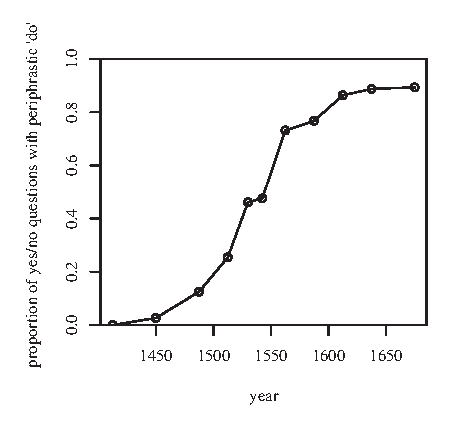
\includegraphics{scurve}
\caption[Competition between two syntactic patterns of \emph{yes/no questions}, as observed in a corpus of Middle English writing]{Competition between two syntactic patterns of \emph{yes/no questions}, as observed in a corpus of Middle English writing~\citep{Ellegard1953}. The established question syntax~(e.g.~``Went he?'') was gradually replaced by its modern variant~(e.g.~``Did he go?'') along an s-shaped trajectory.} 
\label{fig:scurve}
\end{figure}

\subsection{Language-internal accounts}

In order to explain \emph{why} languages change, many studies have attempted to pin down the causes of individual changes by systematically comparing the states of the languages prior to and after a change~\citep{Hockett1965,McMahon1994}. While many of the earliest such studies would attribute change to the gradual accumulation of performance and transmission errors alone~\citep[e.g.][]{Jespersen1922,Hockett1958}, the generativist paradigm with its focus on the language acquisition device shifted the attention to child-based language change. Studies of language change in the generative tradition trace changes back to the re-ordering or simplification of a language's grammatical rules~\citep{Kiparsky1968,Wang1969,Bailey1973,Lass1980,Vennemann1983}, 
typically assumed to be due to children's reanalysis of linguistic parameters based on their limited linguistic input~(see~\citet{Kroch2001} and \citet{Foulkes2013} for reviews concerning syntactic and phonological change, respectively).
%e.g.~\citet{Ellegard1953,Lightfoot1979,Kroch1989cr,Lightfoot1991} % not Yang2002
Rather than characterising change as the result of imperfect transmission, a more recent strand of research regards language as a \emph{complex adaptive system} which evolves to fulfill the communicative needs of its speakers, while at the same time adapting to the constraints imposed by their learning mechanisms~\citep{Kirby1999,Steels2000,Griffiths2007,LCAS2009}.

What unites these \emph{language-internal} accounts is that they all rely on a qualitative difference between the language states prior to and after the change. This difference can be based on a variety of factors, such as the languages' expressivity, processing efficiency, or simply their stability with respect to error-prone language acquisition. Within historical and variationist linguistics such explanations of language change have long been criticised on the basis that they \emph{overpredict} change~\citep{Saussure1959,Greenberg1959,Weinreich1968,Lass1980,Ohala1989,Croft2000,Labov2001,Winter-Froemel2008}. In their seminal paper, Weinreich~et~al. succinctly summarised the issue and coined it the \emph{actuation problem}: ``Why do changes in a structural feature take place in a particular language at a given time, but not in other languages with the same feature, or in the same language at other times?''~\citep[p.102]{Weinreich1968}.\index{actuation!actuation problem}

In other words, language-internal pressures by themselves do not account for the \emph{sporadicity} of language change: many non-adaptive or suboptimal structures that are claimed to have been selected against in one language will happily persist in other languages -- and when they finally do change, language-internal accounts often offer no explanation of what triggered the \emph{actuation} of the change~\citep{Saussure1959,Postal1968,Ohala1993}. While language-internal factors offer good predictions of \emph{which} changes are more likely to occur than others~\citep{Jaeger2010,Wedel2013short}, they do not explain \emph{when} or \emph{why} the stable transmission of language suddenly caves under functional pressures when it does. To account for the sporadic nature of language change, many have argued that it is not enough to rely on intra-linguistic factors alone.%~\citep{Weinreich1968,Croft2000}.

\subsection{Social accounts}

Sociolinguistic research of the past five decades has shown that innovations do not spread uniformly across a given speech community, but that the progression of change is stratified based on factors such as a speaker's age, ethnicity, or socio-economic status~\citep{Foulkes2006,Tagliamonte2012}. \emph{Social accounts} hold that social features of linguistic variants, rather than their inherent linguistic character, are responsible for driving language change~\citep{Sturtevant1947,Croft2000,Labov2001,Croft2006}. Social accounts of language change are \emph{evolutionary} in nature: they decouple the generation of \emph{variation} from the process of \emph{selection} which leads to the diffusion of variants through a speech community. \index{selection}
The underlying mechanisms, however, are very different from biological evolution. While the generation of new variants is assumed to be driven by linguistic or functional factors, social accounts attribute the ultimate \emph{selection} of variants to extra-linguistic social factors~\citep{Ohala1989,Croft2000,Labov2001,Stevens2013}. The `division of labour' between language-internal and social pressures in this approach can simultaneously account for the arbitrary adoption of one linguistic convention from the pool of variants over another, while at the same time explaining the crosslinguistic distribution of linguistic features which reflect functional pressures.
%In general cultural evolution terminology, functional pressures generate a pool of variants that is skewed towards, 

Recent work on a mathematical model of language change suggests that only the presence of a bias which favours the replication of a newly incoming variant can reliably reproduce the s-shaped transitions observed in language change~\citep{Blythe2012}. While this mechanism, known as \emph{replicator selection}, is in principle also compatible with language-internal biases, the authors eschew this conclusion. In line with social accounts of language change they conclude instead that it is the \emph{social prestige} of a new variant that is responsible for its preferential replication. Importantly, the sociolinguistic use of the term \emph{prestige} actually refers to a \emph{content bias}: \index{prestige!variant prestige}
rather than preferentially copying variants used by prestigious individuals, \emph{prestige} is simply another name for a bias that, while social in origin, is actually inherent to the linguistic variant~\citep{Sturtevant1947,Labov2001}. Crucially, social accounts do not solve the underlying logical problem of how a population would agree on the selection of a new variant if there is no objective advantage to that variant. The choice of the population to attach preferential prestige to some variant is as arbitrary and requires just as much explanation as the population's increased use of one linguistic variant over another. Because variant prestige is not accounted for within the theory~\citep{Meillet1921,Labov2001} and can only be attributed post-hoc~\citep{Sankoff1988,Trudgill2004,Maegaard2013}, social accounts are typically unable to make a priori predictions about whether particular changes are likely to happen or not. If we saw competing variants as completely identical in terms of both their linguistic \emph{and} social value, % fitness
how could directed transitions come about? To address this question, it is useful to consider ideas from the wider domain of cultural evolution.

\subsection{Replicator-neutral accounts}\index{neutral evolution}

The evolutionary approach to language variation and change outlined above has also been adopted widely to study processes of cultural change more generally~\citep{Boyd1985,Mesoudi2011}. Interestingly, even though replicator-neutral accounts -- where individuals have no inherent preference for any of the competing variants -- have been studied extensively in the context of cultural evolution~\citep{Bentley2004,Bentley2007}, such models have received relatively little attention in the study of linguistic change~\citep[e.g.][]{Trudgill2008,Baxter2009}.

One of the attempts to build a bridge between general models of cultural evolution and the dynamics of language change is~\citet{Reali2010}. Starting from a model of pure neutral evolution by random copying -- where individuals replicate the different variants proportionally to their current frequency -- the authors add what they frame as an inferential bias for \emph{regularisation}. %, i.e.~a slight preference for individuals to adopt grammars exhibiting no variation.
They show that the trajectories produced by this `regularising' neutral model exhibit s-shaped growth, as long as only those trajectories initiated at 0\% use of a novel variant and terminating at 100\% use are considered. Crucially, however, their mathematical model captures all possible trajectories between those two points, and their result holds only for the \emph{average of all possible trajectories}. This idealised trajectory is highly unlike the `typical' transitions produced by their neutral evolution model, which are characterised by a noisy trajectory, often with many reversals. The strict symmetry of their Markov model also predicts that there should be as many completed language changes as there are actuated changes that went to the 50\% mark before being interrupted, a situation that does not seem to be the case. These considerations call into question whether neutral evolution by random copying can provide an adequate model of the dynamics of language change~\citep{Blythe2012neutral}.

While in pure neutral evolution models the likelihood of replicating a variant is assumed to be dependent on that variant's current frequency alone, another class of replicator-neutral models that has received increased attention recently considers the effects of \emph{temporal information} and \emph{memory} on the diffusion of cultural traits. % (and particularly linguistic)
\citet{Labov2001} for example suggested that the systematic incrementation of sound changes across generations could be explained by the notion of \emph{age vectors}.\index{age vector}
He hypothesises that, following an initial stage where learners acquire the average community usage of linguistic variants, adolescents advance their productions in line with the age stratification of variable usage that can be observed in the population -- in other words, it presumes that youngsters have a bias against sounding \emph{outdated}. This idea was taken up by~\citet{Mitchener2011}, who framed it in terms of \emph{prediction-driven instability}: in his mathematical model, individuals are able to observe the usage levels of a categorical sociolinguistic variable among the `older' and `younger' individuals in the population. New individuals entering the population then adopt a usage rate according to the predicted future use of the variants, by extrapolating from the usage levels of the two groups along an idealised logistic curve. While the model exhibits spontaneous transitions between the two (or more) competing language states, it produces trajectories that exhibit rapid growth from the onset of the change, unlike the gradual uptake observed in empirical data such as shown in~Fig.~\ref{fig:scurve}. %The model also relies on individuals not changing their usage frequencies once they are added to population, i.e.~
The individuals' usage rates also remain fixed after they are initally acquired, leaving open the question of whether the same mechanism could also give rise to directed changes when individuals adjust their usage rates throughout their lifetime, as has been observed in linguistic changes~\citep{Sankoff2007}.

Another general model of cultural evolution based on a similar principle is \emph{momentum-based selection}~\citep{Gureckis2009}, which we will study more closely in the remainder of the current analysis. In this model, an individual's choice between competing cultural variants is influenced by the variants' \emph{momentum}, i.e.~by \emph{changes to the variants' frequency of use} in the recent past.\index{momentum} Individuals are assumed to be biased towards variants which have recently seen an increase in their usage rate, and conversely biased against variants that have been adopted relatively less frequently in the recent past.

\citeauthor{Gureckis2009} test their model on a dataset of the frequency of names given to children in the US over 127~years. Their prediction for the popularity of a name in a given year, which is based on the name's long-term popularity modulated by its short-term momentum, leads to a significantly better fit of the empirical data than the prediction made by pure random copying accounts which do not incorporate momentum. Importantly, their model was primarily intended to be fit to empirical data, but not meant as a generative model of individual behaviour. The authors rule this out, noting that ``if rising names are preferred, which in turn causes them to rise, then a momentum bias might quickly lead to convergence on a single token''~(p.668). They regard this as a negative property of the model, as they are interested in mechanisms that exhibit \emph{cycles} in the popularity of traits, such as found in the realm of fashion~\citep{Kroeber1919,Berger2009,Acerbi2012}. In language, on the other hand, convergence on a single convention is the rule rather than the exception, suggesting that momentum-based selection may be an appropriate model for language change.

\section{Momentum-based selection}

Our main contribution in this work is to investigate the dynamics of momentum-based selection by integrating it into an existing framework of language change, and evaluating it with respect to the characteristics of language change we identified above: the \emph{sporadic} nature of changes which, once actuated, proceed in an orderly, \emph{directed} manner. We begin by reviewing the original formulation of momentum-based selection in~\citet{Gureckis2009}. The model is built around tracking exponentially weighted moving averages~(EWMAs) of the relative frequencies of competing cultural traits over time. Given a time series of relative frequencies~$\vec{n}=\langle n_1, n_2, n_3,\dots\rangle$, the weight of each data point towards the moving average, which we denote~$\hat{n}_\alpha(t)$, decreases exponentially over time (hence the name). %The initial value is typically set to the value of the first datapoint, i.e. $\hat{n}_\alpha(0)=n_{0}$.
Given a new datum~$n_t$ received at time~$t$, the moving average is updated iteratively using
\begin{equation}\label{eq:ewma}
\hat{n}_\alpha(t) = \alpha\cdot n_t + (1-\alpha)\:\cdot\:\hat{n}_\alpha(t\!-\!1)\;.
\end{equation}

The parameter $\alpha\in[0,1]$ is a smoothing factor that determines both the weight given to the newest data point, as well as how quickly the data points' weight decreases over time. At time~$t$, the relative weight of datum $n_{t-i}$ to the current average is $\alpha\cdot(1-\alpha)^i$. The higher~$\alpha$, the more weight is given to more recent data points. Based on this, the momentum of a variant at time $t$, $m(t)$, is determined by calculating two EWMAs $\hat{n}_\alpha(t), \hat{n}_\gamma(t)$ of the variant's attested frequencies $\langle n_1\cdots n_t\rangle$ with two distinct smoothing factors~$\gamma>\alpha$, and taking their difference,
\begin{equation}
m(t) = \hat{n}_\gamma(t) - \hat{n}_\alpha(t).
\label{eq:momentum}
\end{equation}
Because the higher $\gamma$ gives more weight to recent data points, the moving average $\hat{n}_\gamma(t)$ corresponds to the more recent popularity of a trait while $\hat{n}_\alpha(t)$ captures its long-running popularity. The momentum term $m(t)$ will consequently be positive if a variant has been more popular in the recent past compared to its long-term popularity, and negative if the variant has been adopted relatively less frequently in the recent past.

\subsection{Mathematical properties of momentum}

To understand just what is captured by the momentum term~$m(t)$, we can investigate the general dynamics of the difference between two EWMAs $\hat{n}_\alpha(t), \hat{n}_\gamma(t)$ based on their parameters $\gamma>\alpha$. %~\footnote{Readers who are not interested in the mathematical details of the model may wish to skip to the next section.}.
The strongest possible trend in changes to relative variant frequency can be achieved by initialising both EWMAs so that they indicate categorical usage of, say, the outgoing variant~(i.e.~$\hat{n}_\alpha(0)=\hat{n}_\gamma(0)=0$), and then continuously updating both EWMAs with input data suggesting that, actually, everyone is using the novel, incoming variant categorically (i.e.~$\vec{n}=\langle1,1,1,\ldots\rangle$). Even in this simple case, the dynamics of the momentum term are complex, as can be seen in Fig.~\ref{fig:ewmadifference}.

For the underlying EWMAs themselves, the higher the smoothing factor, the faster they approach the input values~(Fig.~\ref{fig:ewmadifference}a.i), and the more quickly they reflect changes in the distribution too~(Fig.~\ref{fig:ewmadifference}a.ii). The corresponding momentum terms that are derived by subtracting an EWMA with a high parameter~$\gamma$ from a more slowly changing one with a lower parameter~$\alpha$ are shown directly underneath~(Fig.~\ref{fig:ewmadifference}b). What is of interest to us are the different \emph{shapes} of these momentum curves: a parameter combination which exhibits a rapidly rising curve will cause an individual to posit a trend based on just a few suggestive input data points, while a curve that slopes off slowly means that a momentum bias will persist for a longer time after the initial detection of a trend.

Both the number of data points it takes to reach their maximum value as well as the amplitude of this highest possible momentum value depend on both smoothing factors in complex ways. The short-term memory parameter~$\gamma$ is of particular importance, as it controls the time depth at which the momentum term is most sensitive to underlying trends in the data: a high~$\gamma$ causes the momentum term to immediately reflect short-term variation in the input, while settings of~$\gamma$ closer to~$\alpha$ lead to more conservative trend estimates which smooth over the noise present in individual input data points.

The sudden change in trend after 60~data points shown in Fig.~\ref{fig:ewmadifference}b.ii illustrates this point: a momentum term based on high $\gamma=0.15$~(dotted line), while very quick to reflect sudden changes in the input, is very unstable. After receiving only five data points of the new input value $n_t=0$, the previous sustained upward trend is `forgotten', with the momentum term first quickly returning to $0$, then going negative to reflect the new, short-term downwards trend from the series of 1s back to 0s. %Momentum terms based on settings of $\gamma$ closer to $\alpha$~(e.g.~$\gamma=0.02$, dashed line) are more conservative, requiring sustained evidence of a trend over time to reach a high value.

%A value of $\gamma$ further away from $\alpha$ decreases the time until the maximally possible momentum is reached while making the overall time-course of momentum more peaky, with a higher maximum value and quicker decay back towards~$0$ following the peak.

\begin{figure}
\centering
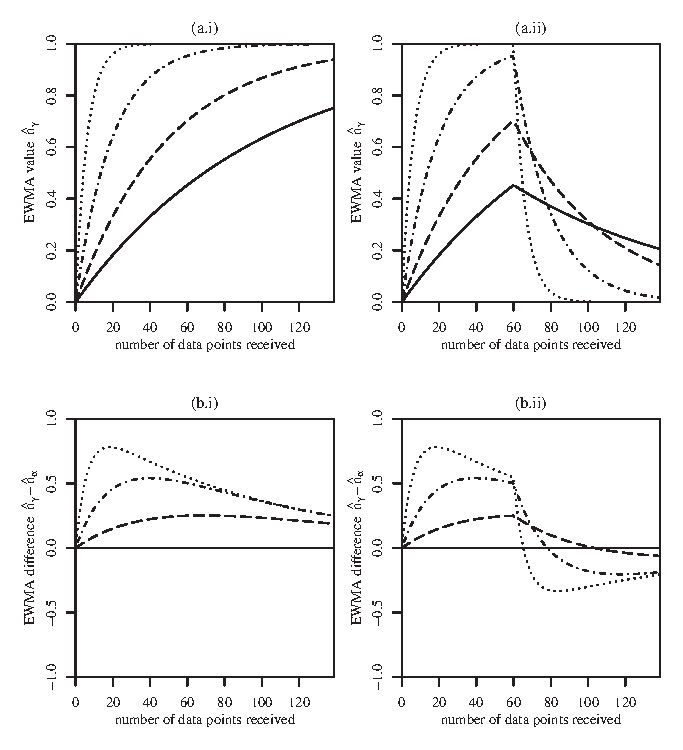
\includegraphics{ewmadifference}
\caption[Exponentially weighted moving averages~(EWMAs) of the same input data but with different smoothing factors, as well as their corresponding momentum terms]{Exponentially weighted moving averages~(EWMAs) of the same input data but with different smoothing factors, as well as their corresponding momentum terms.
% ; the slowest (solid) line shows the development of the EWMA with $\gamma=.01$, the fastest~(dotted) line $\gamma=.15$
\textit{(a.i)}~Four EWMAs with smoothing factors $\gamma=0.15, 0.05, 0.02, 0.01$~(from top to bottom) are initialised at $\hat{n}_\gamma(0)=0$ and repeatedly updated using the same constant input data series $\vec{n}=\langle1,1,1\dots\rangle$. \textit{(a.ii)}~same as~(a.i), but with the input data series $\vec{n}$ switching from all $1$s to all $0$s after 60 data points. %The EWMAs with the highest decay parameter quickly converge back towards the new input target $0$.
\textit{(b)}~Corresponding momentum terms~$m(t)=\hat{n}_\gamma(t)-\hat{n}_\alpha(t)$ derived from the trajectories above, by taking each EWMA and subtracting the value of the EWMA with the lowest smoothing factor from above~($\alpha=0.01$). Line styles correspond to those in~(a).}
\label{fig:ewmadifference}
\end{figure}

Generally, assuming an abrupt change in the input values such as above, the number of iterations that both EWMAs have to be updated with the same constant input value before the maximum possible difference between the two is reached is
\begin{equation}
t_{\rm mmax}(\alpha,\gamma)=\frac{\ln\frac{\alpha}{\gamma}}{\alpha-\gamma}\;.
\end{equation}

The maximum possible amplitude of the momentum term at that point is
\begin{equation}
m_{\rm max}(\alpha, \gamma)=e^{-\gamma t_{\rm mmax}(\alpha,\gamma)}-e^{-\alpha t_{\rm mmax}(\alpha,\gamma)}\;.
\end{equation}

Knowing the mathematical boundaries of the momentum term~$m(t)$ we can now go on to incorporate the momentum bias into a model of language change.

\subsection{The Utterance Selection Model of language change}\index{Utterance Selection Model}

To investigate the dynamics of momentum-based selection as a model of individual behaviour, we implemented the momentum-based selection bias in the \emph{utterance selection model} of language change~(USM)~\citep{Baxter2006,Blythe2012}. Derived from \citeauthor{Croft2000}'s evolutionary theory of language change~(\citeyear{Croft2000}), the USM provides a well-studied multi-agent framework to study the dynamics of the competition and diffusion of \emph{discrete} linguistic replicators, be they lexical items, constructions, or different categorical variants of a speech sound\footnote{For an account of how age vectors can drive change in a continuous dimension such as vowel productions, see~\citet{Swarup2012}.}.

Two fundamental principles underlie the design of the USM: firstly, the individual agents use the competing variants \emph{proportionally}, rather than categorically. In the minimal case with only two competing variants studied here, an agent's usage rates can be fully described by a single number, call it~$x$, in the range~$[0,1]$.
While this value can be interpreted as reflecting some cognitive state of the speaker, it also has a more direct behavioural correspondent: when an agent is selected to participate in an interaction, their probability of producing the novel variant is equal to~$x$, while the probability of producing the competing variant is~$1-x$. This aspect of the USM is in line with linguistic evidence which shows that human language use is inherently variable and probabilistic~\citep{Kroch1994,Labov1994,Bybee2007,Nardy2013}.

Secondly, agents continuously tune their own variable usage rate towards the production rates they observe in interactions with other agents, thus mimicking the human tendency to \emph{align} linguistic behaviour with that of interlocutors~\citep{Giles1991,Branigan2000,Jaeger2013}. This aspect of the USM is in line with the finding that many aspects of linguistic behaviour do not remain fixed, instead remaining malleable across an individual's life span~\citep{Kerswill1996,Sankoff2007,LCAS2009,Bowie2013,Stanford2014handbook}. According to the formal definition of the USM~\citep{Baxter2006}, an agent's current proportion of use of a variant $x_\alpha(t)$, is simply an exponentially weighted moving average~(EWMA) of the frequencies of the incoming variant that the agent has observed in their input over time\footnote{For simplicity of notation we will henceforth omit the $\hat{}$ above the variables denoting EWMAs.}. The rate of alignment is controlled by the smoothing factor~$\alpha$ of this EWMA, which can be understood as a \emph{learning rate}. This learning rate is typically held small~(in the range of~$0.01$): there is alignment, but the individual frequency adjustments after an interaction are very small and it takes many interactions for an agent to change their preferred variant.

On top of this basic update rule, a USM agent's alignment behaviour can be altered by applying biases to their input data before it gets incorporated into the EWMA. This is where momentum-based selection comes into play.

\subsection{Momentum-based selection in the USM}

We now explain how to minimally incorporate momentum-based selection into the USM. Assuming an agent using learning rate~$\alpha$ has just engaged in its $t$-th interaction and observed another agent use the incoming variant with a relative frequency of~$y$, then their own frequency of use $x_\alpha$ is updated to be
\begin{equation}
x_\alpha(t) = \alpha\cdot f(y) + (1-\alpha)\cdot x_\alpha(t\!-\!1)\;,
\label{eq:usm}
\end{equation}
where $f(y)$ is a function from $[0,1]$ to $[0,1]$ which transforms the \emph{objective} observed frequency~$y$ of the variant into a subjective \emph{perceived frequency} which the agent then aligns to. 
Similar to \cite{Gureckis2009} we can now simply define the perceived frequency~$f(y)$ of an agent in the momentum-based USM as the objective frequency~$y$ of a variant observed in an interaction offset by that variant's momentum,
\begin{equation}
f(y) = y + b \cdot m'(t)
\label{eq:momentumusm}
\end{equation}
with the exception of
\begin{equation}
f(0)=0 \quad {\rm and} \quad f(1)=1\;.
\label{eq:momentumusmconstraint}
\end{equation}
We impose the latter since our focus lies on modelling the diffusion of existing linguistic variants, independent of how those variants were introduced into the population to begin with. It simply stops our momentum-biased selection function~$f(y)$ from introducing novel, unattested variants, a constraint that is typical of models of selection generally~\citep[see e.g.][]{Boyd1985}. The positive bias parameter~$b$ in equation~\ref{eq:momentumusm} controls the strength with which the normalised momentum term $m'(t)$ as defined below in Equation~\ref{eq:normalisedmomentum} influences the perceived frequency. Should the momentum bias cause~$f(y)$ to go below~$0$ or above~$1$, it is simply truncated at~$0$ and~$1$, respectively\footnote{The exact form of the bias function $f(x)$ matters much less than its monotonicity and the fact that $f(x)>x$ when the momentum term is positive (i.e. when the agent perceives an upward trend) and $f(x)<x$ when it is negative (indicating a downward trend).}. Crucially, because the momentum term can be positive or negative~(depending on the direction of the trend), this perceived frequency function is \emph{symmetric}, which makes it \emph{replicator-neutral}: no matter which bias strength~$b$ is used, the function does not a priori favour one of the variants over the other.

Since the effect of different strengths of this bias parameter~$b$ on the model dynamics is relevant to our analysis, we have to make sure that its settings are comparable across settings of the other parameters. This isn't as straightforward as it might seem, because the range of values that the original momentum term definition~$m(t)$ in Equation~\ref{eq:momentum} can take on depends on both smoothing factors~$\alpha$ and~$\gamma$, as could be seen in Fig.~\ref{fig:ewmadifference}. The absolute amplitude of the momentum curves is of little interest to us; on the contrary, the differences in maximum possible amplitude distort the effect of the bias parameter~$b$ which is supposed to control the strength with which momentum is applied. To counteract this, we normalise the momentum term~$m(t)$ based on the $\alpha, \gamma$ used in a given simulation condition. For any given pair of smoothing factors $\alpha, \gamma$, we can scale the momentum term to the~$[-1,1]$ range by defining the normalised momentum
\begin{equation}
m'(t)=\frac{x_\gamma(t) - x_\alpha(t)}{m_{\rm max}(\alpha, \gamma)}\;.
\label{eq:normalisedmomentum}
\end{equation}

% TODO
To calculate the momentum component in the numerator, the difference between two EWMAs, we simply re-use the agent's own usage frequency, which according to the USM definition is also an EWMA. To augment the basic USM with momentum-based selection, every agent simply has to keep track of another~$x_\gamma$ on top of the long-term estimate~$x_\alpha$ it already maintains.


\section{Results}

\subsection{Analytical approximation}

Before proceeding to a full population-based simulation we can establish the general dynamics of the model by investigating the behaviour of an individual agent set in an idealised, deterministic production-perception loop~\citep{Wedel2006}.\index{production-perception loop}
We initialise a single agent to use the incoming variant at some low level and repeatedly update their two EWMAs $x_\alpha(t), x_\gamma(t)$ by having them align to their own proportion of use~$x_\alpha(t)$ for 100~iterations. As can be seen in Fig.~\ref{fig:feedbackloop}, nothing happens: an agent aligning to their own usage rate simply remains at that proportion and, in the absence of any changes in the input sequence, the momentum term stays~0. To test how the model reacts to fluctuations in the input we alter the agent's input by fabricating a data point which suggests that their interlocutors are actually categorically using the incoming variant~(see Fig.~\ref{fig:feedbackloop}a). When the agent aligns to this input it leads to a small punctual increase in their variant use, but the sudden change in the input data also makes the momentum term take on a positive value~(dashed grey line).
% Continuous alignment to the agent's momentum-influenced \emph{perceived} usage level~(dashed black line) leads to some further increase in the usage rate before the momentum bias tapers off towards~0.%~(
Following the fabricated data point, the agent again receives their own samples as input data. But the bias exerted by the momentum term, which makes the agent's \emph{perceived} usage rate higher than their actual usage rate, causes further increases in their use of the incoming variant. However, the lack of further perturbations causes the momentum to decay back towards~$0$, and the agent becomes stationary again at a usage level not far from their initial setting. If we introduce a second fabricated data point shortly after the first one, the model's behaviour changes dramatically: the system enters a regime where the momentum bias generated by the two fabricated data points affects the perceived frequency of the agent's input so much that it causes the momentum term to increase even further, leading to self-reinforcing runaway change~(Fig.~\ref{fig:feedbackloop}b).

\begin{figure}
\centering
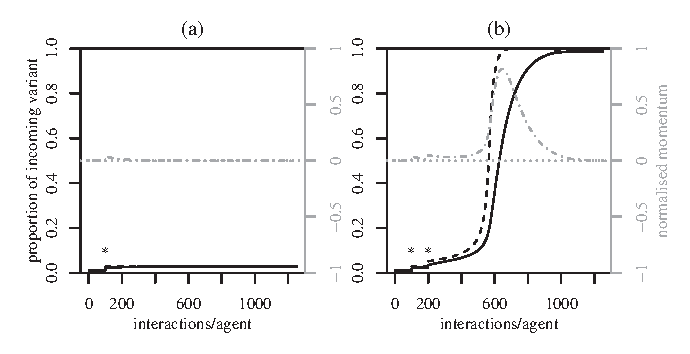
\includegraphics{feedbackloop}
\caption[Momentum-based selection dynamics of a single agent's usage rate in a deterministic production-perception loop]{Momentum-based selection dynamics of a single agent's variable usage rate in a deterministic production-perception loop, with learning rates $\alpha=0.01, \gamma=0.02$ and momentum~bias~$b=2$. At every time step the agent updates their own usage rate~(solid black line) by aligning to their own average momentum-biased production with a sample resolution of~$T=5$~(indicated by the dashed black line). This stable loop is perturbed by administering fabricated input data suggesting 100\% usage of the incoming variant at the time points marked by asterisks, demonstrating the two regimes of momentum-based selection: \textit{(a)}~stability: a single fabricated data point after 100~interactions causes a sudden increase in the agent's usage rate~(solid black line) as well as the momentum term~(dot-dashed grey line, right axis), but the feedback loop stabilises again. \textit{(b)}~directed transitions:~adding another fabricated data point after 200~interactions raises the momentum term high enough to trigger self-reinforcing runaway change, giving rise to an s-shaped transition.}
\label{fig:feedbackloop}
\end{figure}

This preliminary analysis shows that the momentum-based selection model exhibits two different regimes, accounting for both periods of stability and of directed change. Capturing the dynamics of the transition between the two regimes is however not trivial: particularly the switch from stability to a directed transition depends crucially on both the strength of the momentum bias as well as random fluctuations in the agents' input as they sample data from their interlocutors. We therefore turn to numerical simulations, where the data production and agent interactions will be driven by stochastic processes.

\subsection{Numerical simulation}

In order to get a fuller picture of the momentum-based selection dynamics we ran simulations with a total of 2,520~parameter combinations\footnote{The source code for running the simulations as well as the analytical approximation are available at \url{http://github.com/kevinstadler/momentum}}. The six parameters of the momentum-based USM are summarised below. Only one, the learning rate~$\alpha$, was held constant across all simulation runs, the other five parameters were varied at the levels given in parentheses:

\begin{itemize}
\item[-] $\alpha$: the agents' learning rate ($0.01$)
\item[-] $\gamma$: the agents' short-term memory smoothing factor~($0.015, 0.02, 0.025, 0.03, 0.35, 0.4$)
\item[-] $T$: the Binomial sample size determining the resolution at which agents can observe each other's relative usage frequencies~($2, 3, 4, 5$)
\item[-] $b$: the bias strength with which agents apply the normalised momentum to yield their \emph{perceived} frequency of usage~($0.5, 1.0, 1.5, 2.0, 2.5$)
\item[-] $N$: number of agents in the population~($2, 5, 10, 20, 30, 50, 100$)
\item[-] $x_0$: initial proportion of the incoming variant used by all agents~($0.01, 0.02, 0.03$)
\end{itemize}

Combining all these possible parameter combinations and running the 2,520~conditions for 48 trials each resulted in a total of 120,960~simulation runs. On top of the conditions listed above, we also produced simulation runs where we set the bias strength~$b=0$, which is equivalent to pure neutral evolution. 24,192~runs from this additional condition provide a baseline that the dynamics of our momentum-based selection model can be compared against. Every simulation run proceeds as follows:

Firstly, initialise $N$ agents, setting both their $x_\alpha$ and $x_\gamma$ to $x_0$. Then, carry out interactions between agents by repeating the following steps:

\begin{enumerate}
\item randomly select two agents $i, j$ from the pool of $N$ agents -- we assume that all pairs of agents have the same probability of interacting with each other.
\item let both agents produce $T$ tokens of the variable by taking a random sample $n_i, n_j$ for each agent from the Binomial distribution $B(T, x_\alpha)$, using the two agents' respective usage rates~$x_\alpha$ at the time of the interaction.
\item calculate the perceived frequencies that the agents will align to, using equation~\ref{eq:momentumusm}. For agent $i$, who will align to $j$'s productions, calculate $f(\frac{n_j}{T})$ using agent $i$'s current normalised momentum term~$m'(t)$; for agent $j$, calculate $f(\frac{n_i}{T})$ using $j$'s~$m'(t)$. %The model parameter~$b$ controls the strength with which the respective agents' momentum term~$m'(t)$ is applied.
\item update both agents' $x_\alpha$ as well as $x_\gamma$ by incorporating their perceived frequency according to equation~\ref{eq:usm}.
\end{enumerate}

The simulations were run until every individual in the population had converged to within a ten-thousandth of a percent of using only one of the two competing variants, or for a maximum of 200,000~interactions per agent\footnote{More than~$99\%$ of simulation runs had terminated before this time limit was reached.}.

\subsection{Simulation results}

For the sake of our analysis we use a simple definition of what a `transition' is. Taking a fixed threshold~(say 5\%), we can define the two extreme areas where the mean population usage level of the minority variant is below this threshold as the two regions of `near-categorical use' of either variant. A transition, then, is the period in which the mean usage levels of the population crosses from near-categorical use of one to near-categorical use of the other variant. A first striking finding when analysing the simulation results is that changes are rare: of the 120,960~simulation runs using the momentum bias, only 18,040~(around~15\%) ever exhibit a transition, while the majority of runs simply converge on categorical use of the majority variant. This result is in line with the observation that the actuation of language change is \emph{sporadic}: even when a novel variant is known to the entire population, this alone is not likely to lead to a community-wide language change.

\begin{figure}
\centering
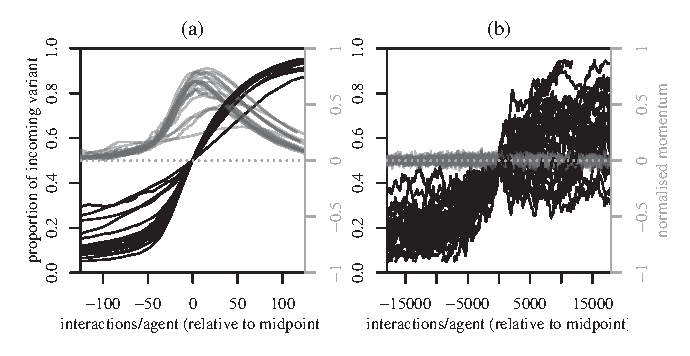
\includegraphics{alltransitions}
\caption[Successful transitions generated by simulation runs in conditions with and without the momentum-based selection bias]{Successful transitions generated by simulation runs in conditions with and without momentum-based selection. The graphs show the development of the average proportion of use of the incoming variant across the population~(black line, left axis) from the point where it crosses the 5\% mark until it reaches 95\%, alongside the average momentum term during that period~(grey line, right axis). Transitions are aligned at the point where the trajectory first crosses the $50\%$ mark of incoming variant usage. \textit{(a)}~20~trajectories randomly drawn from the 21,909 successful transitions generated by momentum-based selection with momentum bias~$b\ge1$, population sizes $N\ge5$ and various settings of $\gamma, T, x_0$. %The momentum term influences the agents' perception of the usage levels around them which, once triggered, leads to a self-reinforcing feedback loop.
\textit{(b)}~all 28 transitions generated in 17,280~simulation runs with $b=0$, equivalent to neutral evolution, with various settings of $\gamma, T, x_0$ and population sizes~$N\ge5$. %Without the influence of the momentum bias, transitions become both much rarer and slower as population size increases~
Note the different time scales. The momentum term, ineffective when~$b=0$, is shown for reference.}
\label{fig:alltransitions}
\end{figure}

When we investigate the distribution of transitions across the different parameter settings, we find that the bias strength~$b$ carves the space into two regions with distinct dynamics: while simulation runs with $b\ge1$~exhibit directed transitions at comparable time scales, the neutral evolution condition with $b=0$ as well as the weak momentum bias setting at~$b=0.5$ yield both fewer and temporally less consistent transitions, as shown in Fig.~\ref{fig:alltransitions}. The difference between those two regimes is exacerbated as population sizes become larger, making transitions in the neutral evolution conditions even rarer and slower.

Beyond this qualitative difference in successful transitions, our earlier prediction regarding the general directedness of trajectories in the neutral evolution condition are also borne out by the results: of all simulation runs where the incoming variant ever reaches the half-way mark~(i.e.~average $50\%$~usage of both variants across the population), only $55\%$ of trajectories in conditions with $b\le0.5$ actually result in the diffusion of the incoming variant. The remaining half-completed transitions are interrupted and revert back to majority usage of the established variant. In contrast, in conditions with $b\ge1.0$, $97\%$~of the trajectories that reach the half-way mark also lead to the population-wide adoption of the incoming variant.

In contrast to the low-bias conditions which exhibit the dynamics of neutral evolution, conditions with a sufficiently high momentum bias~$b$ reliably produce s-shaped transitions between the two regions of near-categorical use at irregular intervals.
%Transitions occur in both directions, which is expected given 
before eventually converging on categorical use of either of the variants. The dynamics are robust under many different parameter settings which give rise to highly similar transition dynamics~(see Fig.~\ref{fig:alltransitions}; the parameters' much greater influence on the likelihood of transitions occurring is beyond the scope of this paper). While similar transitions are also found in models driven by replicator selection, an important difference is that our model has no a priori preference for any of the variants built in. Instead of having a constant bias applied from outwith the model, the momentum term provides the opportunity for a bias to emerge dynamically from within the system, as can be seen from the temporal development of the momentum term in Figs.~\ref{fig:transitions}. Crucially, rather than relying on an external trigger, the s-shaped transitions are \emph{self-actuating}: agents constantly read weak trends into the random fluctuations in their input but these temporary individual biases will vary across the population, and more often than not cancel each other out. There is, however, always the possibility for these weak biases to overlap, which could cause a subset of agents to slowly shift their variant use in parallel. When this shift is detected by other agents they will themselves start to amplify it, leading to a self-reinforcing feedback loop. The directed transitions in a momentum-based model of language change are triggered \emph{spontaneously} and, while it is the most likely outcome, changes are not guaranteed to succeed either: even if a change is actuated, its propagation is not completely inevitable, as can be seen in interrupted changes such as the one shown in Fig.~\ref{fig:transitions}b. The dynamics of momentum-based selection provide an intriguing account of the unpredictability of the actuation of linguistic changes without the need for an external bias or trigger.

\begin{figure}
\centering
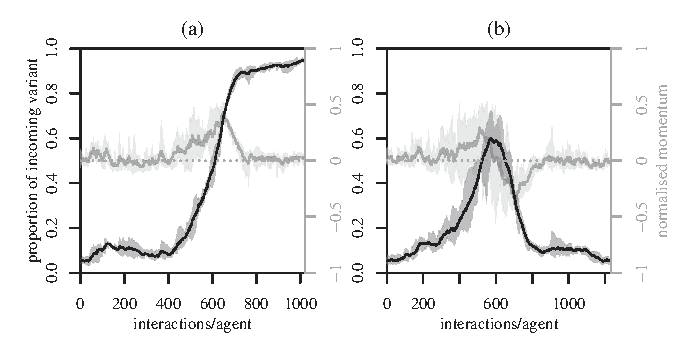
\includegraphics{transitions}
\caption[Successful and unsuccessful transitions generated by two simulation runs using identical parameter settings]{Transitions generated by two simulation runs using identical parameter settings~($N=5, b=2.0, T=2, \alpha=.01, \gamma=.04$). The graphs show the development of the average proportion of use of the incoming variant across the population~(black line, left axis) as well as the average momentum term influencing the agents' perception~(grey line, right axis). Shaded intervals indicate the range~(minimum and maximum values) attested in the population. \textit{(a)}~A successful, s-shaped transition typical of momentum-based selection: an initially noisy momentum value rises high enough to trigger self-reinforcement of the momentum bias~(at around 450~interactions) until it saturates and tails off again \textit{(b)}~Example of a rare, interrupted transition: despite the onset of a directed shift, the wide range of momentum biases across the population destabilises the feedback loop, causing the average momentum to break down and invert, returning the usage frequency of the incoming variant back towards its initial low level.}
\label{fig:transitions}
\end{figure}

The trajectories shown in Figs.~\ref{fig:transitions} are exemplary of the dynamics of momentum-based selection across the full range of parameter settings we explored. Only for settings of the momentum bias~$b$ close to~$0$ as well as for short-term smoothing factors~$\gamma$ very close to the learning rate~$\alpha$ do the momentum-based selection dynamics break down, and the model reverts to pure neutral evolution-like behaviour. In comparison to the prediction-driven model of~\cite{Mitchener2011}, the momentum-based selection model shows that it is not necessary for learners to engage in active prediction of the population's \emph{future} state along a particular trajectory. Rather, having a simple bias based on variant history is sufficient to drive orderly directed changes, and the transitions generated by our model appear to exhibit a more gradual uptake than the trajectories reported by~\citeauthor{Mitchener2011}. We also find that having a bias for \emph{regularisation} is not absolutely necessary to guarantee an orderly progression of the changes. In a population of agents who are continuously updating their usage rates, the momentum bias presented here is robust enough to drive changes to near-completion.

\section{Discussion}

We have shown that the momentum-based selection model fulfills two defining requirements of a model of language change: the spontaneous, sporadic actuation of changes, and their progression in the form of a directed, s-shaped curve. However, other accounts of language change which posit a selection bias in favour of the incoming variant also predict s-shaped trajectories, so how can we know which account best describes the empirical data? While the progression of every instance of language change will be influenced by several factors concurrently or at different times~\citep[see e.g.][]{Ghanbarnejad2014,Stanford2014handbook}, it is still interesting to investigate which (if any) of the mechanisms of language change discussed in the introduction can be identified as the main driving force behind language change. Here, we want to highlight some of the more subtle differences in the predictions made by different accounts of language change which would allow us to tease apart the momentum-based, language-internal and social accounts of language change based on cross-linguistic data.

\subsection{The two rates of linguistic change}\index{rates of change}
\label{sec:tworates}
An interesting (and to our knowledge novel) way to evaluate competing theories of language change is to look at the predictions they make regarding the \emph{rates} of linguistic change. It is important to note that `rate' can refer to two different things in the context of language change: one interpretation of `rate' refers to the probability of a particular change occurring, such as when talking about different English past tense forms becoming regularised over time~\citep{Lieberman2007} or the rate of lexical replacement more generally~\citep{Wichmann2009,Greenhill2010,Monaghan2014}. Rather than referring to the time frame within which a specific change takes place, this really describes the \emph{likelihood of a (type of) change}, or an \emph{actuation probability}. The other use of `rate' refers to the \emph{speed} of the transition of one particular change, i.e.~it is a measure of the time span from the introduction of a new variant to its completely replacing an established one. Under the assumption that language change follows an s-shaped pattern, this second rate of change is often taken to be the growth rate parameter of the logistic function~\citep{Pintzuk2003}, and it is this `rate' that is referred to by the `Constant Rate Effect' observed in syntactic change~\citep{Kroch1989cr}.

What is interesting about these two rates of change is that different accounts of language change make implicit predictions regarding the relationship between them, in particular whether the likelihood of a change occurring is correlated with the rate at which the change proceeds once it has been actuated. Under the assumption that the same pressures that lead to the introduction of more functional or `adaptive' variants are also responsible for their preferred selection once they have been innovated, language-internal accounts would predict that changes which occur more often cross-linguistically should also be selected for more strongly in individual languages. This would translate into faster changes so that, controlling for other factors such as frequency and size of the speech community, the two rates of change should be positively correlated. % according to language-internal accounts.
This differs from the prediction made by the momentum-based account: while the probability of a new variant appearing, and consequently its random actuation from the pool of variants, is dependent on linguistic factors, these factors are not what drives the diffusion of the variant. Assuming that individuals apply similar momentum biases to all linguistic variables, a momentum-based account would therefore predict the speed of individual transitions and the changes' actuation probability to be uncorrelated.

The situation with social accounts is trickier: \index{social accounts}
the fact that many different social factors have been posited to influence the selection of linguistic variants, both positively and negatively, makes it difficult to derive a general prediction regarding the speed of individual changes. What determines the probability of actuation is an equally open question: it has been proposed that the occurrence of changes might be driven by the need to create distinct social identities within a community~\citep{Labov2002,Matthews2012,Roberts2013}, implying that we should not expect actuation probabilities to be constant cross-linguistically.

While it is difficult to derive specific predictions regarding the correlation between the two rates of change from social accounts of language change, many insights into the respective roles of the different pressures could be gleaned from studying cross-linguistic datasets of changes~\citep[see also][]{Bickel2015}. The crucial issue is that the three qualitatively very different accounts discussed here might predict quantitatively similar selection pressures for particular language changes, making it impossible to distinguish the contribution of the different types of pressures on a \emph{per-change} basis. Our understanding of the issue could therefore profit immensely from investigating the empirical distribution of \emph{both} rates of change as well as their relationship based on cross-linguistic data.
%the language-internal and momentum-based accounts can be tested by investigating the correlation between the two rates of change that are attested cross-linguistically.

\subsection{Momentum-sensitivity in the individual}

While momentum-based selection successfully reproduces the macro-level s-shaped curves that are characteristic of linguistic change, this raises the question of whether the model makes valid assumptions about individuals' micro-level behaviour~\citep{Mesoudi2009}. Firstly, it is clear that both linguistic knowledge and performance are embedded in diachrony -- language users are sensitive to changes in the frequencies of variants~\citep{Jaeger2013} and well aware of diachronic connotations~\citep{Labov2001,Guy2003,Tagliamonte2012}, %,Stadler2016SS}
both types of information that could drive momentum-based selection. In the general cultural evolution literature it is well-established that frequency-dependent biases are a natural strategy for social learning tasks, since frequency can be an indicator of the \emph{social value} of a variant~\citep{Boyd1985}. Similarly, \emph{changes} in frequency can be a good indicator of the \emph{future} social value of a cultural variant~\citep{Gureckis2009}. Laboratory experiments on cultural evolution in humans have provided empirical evidence for the self-perpetuating nature of trends, where people will amplify trends even against their own personal preferences~\citep{Salganik2008,Willer2009}, suggesting that individuals might also have an incentive to use metalinguistic information about the history of linguistic variants. While there is plenty of qualitative and anecdotal evidence on speakers' explicit evaluation of language changes~(see~e.g.~\citealt{Trudgill1972,Labov2001,Guy2003,Tagliamonte2012}), quantitative research on the extent of people's explicit or implicit knowledge about the direction of ongoing changes is just starting. Experimental evidence shows that listeners employ their implicit knowledge about ongoing sound changes during speech perception~\citep{Hay2006,Drager2011}, and there is evidence of explicit knowledge both in the area of phonetic~\citep{Carrera-Sabate2014} and syntactic change~\citep{Stadler2016Evolang}. % lexical: Walker2011

%While variationist linguists customarily uncover patterns in the age distribution of linguistic variation based on collected data, quantitative forays 

\section{Conclusion}

In this paper we investigated the \emph{momentum-based selection} model and studied its evolutionary dynamics. Our analysis shows that this model, where individuals are biased towards variants which have recently seen an increase in their frequency of use, exhibits two features characteristic of language change: the spontaneous, sporadic actuation of changes, and their progression in the form of directed, s-shaped curves.

Crucially, the momentum-based selection mechanism demonstrates that the apparent selection of a particular cultural variant in a population is not sufficient evidence for any inherent asymmetry between the variants in competition. Instead, selection biases can be an emergent property of the system, particularly in the case of social learning where individuals possess meta-level knowledge about the variants. The human capacity to acquire meta-linguistic knowledge about ongoing language changes, for example by tracking changes in the variants' frequencies of use over time, therefore deserves further study.

Finally, we highlighted the importance of collecting and studying cross-linguistic data sets of comparable historical changes to test the general predictions made by different accounts of language change. This strand of research in particular needs to be expanded further in order to help us gain deeper insights into the respective roles of the myriad pressures involved in language change.
%on historical language changes as an important source to  
%a number of open empirical questions related to both population-level patterns



% chapter 4
\chapter{Probing momentum-awareness in the individual}
\label{ch:questionnaire}
\section{Introduction}

While the degree to which the historical development of languages is inferred and used by language learners has long been of interest to sociolinguists~\citep{Labov1989}, empirically this question has only been tackled relatively recently as part of a general effort to study the acquisition of sociolinguistic knowledge by individuals~\citep{Labov2014,Foulkes2015}.
Of particular relevance to this thesis is the question of how specific linguistic variants and their relative usage levels can come to be associated with specific age groups.
The concept of `age vectors' captures the age-based stratification of variable usage, and the idea that individual language users possess knowledge of the age vectors of their community has been invoked as an explanation of how language changes are transmitted and increment across generations~\citep{Labov2001}.
The model presented in the previous chapter demonstrated how a similar mechanism, based on tracking changes to frequency distributions of discrete variants in \emph{real time}, can equally account for spontaneous directed transitions of change in a speech community.

While there is an increasing body of empirical evidence on individuals' knowledge of ongoing changes which I reviewed in Section~\ref{sec:agevector}, the experimental data presented there was limited to continuous phonetic changes. Although the fact that this sub-domain of language change still encompasses the largest part of sociolinguistic research might in part be attributed to the generativist sovereignty over morphosyntactic research which did not leave much space for an empiricist-variationist methodology, it is worth noting that the type of sociolinguistic variable (i.e.~whether different variants differ continuously or categorically) influences not just how the linguist might describe or represent variation, but also how that variation is acquired by individuals. %makes a difference, in particular when it comes to enquiring about the \emph{knowledge} about changes.

In particular, the type of variable impacts on the amount of information on inter-individual differences that can be extracted from individual realisations of a variable that is observed in an interaction. While continuous phonetic tokens are potentially very noisy and it might therefore help to have access to a speaker's full distribution of realisations to get a complete picture of their variable usage, given sufficient stratification of variable realisations along a continuous dimension even a single token can potentially contain enough information to place the speaker along a cline from `more outdated' to `more modern' in their variant usage.
Not only that, continuous variants allow speakers to sound `\emph{even more} novel' by extending the change along that cline and producing variants that `overshoot' even the most advanced novel variants, productions which can nevertheless be immediately understood as instantiations of the same innovation.
%\citep{Swarup2012}.
%figure out the age vector between them, in theory you only need as little as one token each from a younger and an older speaker which, given the relative frequency of phonetic variables, should be easy enough to get access to.

The same is not true in the case of categorical variants. Firstly, in order to learn about an individual speaker's variable usage,
%level of participation in a change
one truly need to learn about the overall distribution of realisations, i.e.~the relative frequencies with which the different variants are mixed by the speaker.
Except when different variants are strong social markers which are exclusively used by non-overlapping speaker groups, very little information can be extracted from individual productions. %realisations of a variable.
%which could theoretically be the case for really rapid changes where youngers speakers categorically use only variant that is still unattested in 
Instead, several realisations of a variable by one and the same speaker are necessary to make strong inferences about a speaker.
In combination with the fact that morphosyntactic variables can only be observed much less frequently than most phonetic and phonological ones, 
it is not obvious that people would be as good at acquiring or making inferences about categorical variables as they are for continuous ones, like the vowel realisations tested by~\citet{Drager2011}.

%one sample each you're quite likely to end up with both producing the same token, which is uninformative.

%And to come back to frequency, you also need to wait until you've collected 5+ samples of imperatives with an explicit subject before you can make strong inferences about your speaker, so

%One could argue that all our speakers are doing is learn a simple 'new variant = younger speaker, old variant = older speaker' mapping, but the difference in responses between the imperative and question variables shows that this is not the case: while the reported apparent time differences could be explained by such a simple associative mapping, the fact that the new imperative variant is reported to be used relatively less by *all* speaker groups shows that individuals actually know something about the relative usage of the variants within the individual!

%Beyond the domain of continuous phonetic change,
In one of the rare studies investigating age effects for categorical rather than continuous~(phonetic) traits, \citet{Walker2011} showed the influence of congruence between `word age' and `voice age' in facilitating lexical access: listeners of all ages exhibited a speed-up in processing words produced by a voice indicative of an age group, exactly when the word was more likely to be used by speakers of that age group. %, whether the item or referent were outdated.
Although this experiment speaks to the influence of perceived age directly, it does not involve a sociolinguistic variable, since the different stimuli belong to different semantic domains, rather than being different ways of `saying the same thing'.

%in particular with respect to how variants and usage levels 

%Most traditional accounts of language change are based on the assumption that linguistic divergence occurs during language acquisition, mostly based on language-internal factors that make learners `mislearn' or `reanalyse' their linguistic input, causing them end up with a different target language than that spoken by their caretakers~\citep[see e.g.][]{Salmons2013}. But quantitative research on infants and adolescents has painted a much more refined picture of the \emph{target} of child language acquisition~\citep{Labov2012}. Of particular relevance is the question of how individuals acquire sociolinguistic variation, and how this acquisition develops over time. Quantitative studies of the linguistic patterns of different pre-adolescent age cohorts has shown that, while children's usage patterns might mirror the idiosyncratic language use of their caretakers up until about age three or four, learners then exhibit a pronounced ``outward-orientation'': shedding most of the influence of their caretaker speech, learners instead turn not just towards their peers, but towards the usage patterns in the wider speech community as a whole~\citep{Labov2014}. % also Labov2001, ch.13

The goal of the present work is to extend the body of research on `age vectors', as they are perceived and used by the individual, to the domain of syntactic change. Since this an understudied area of research, we will also present a novel questionnaire methodology designed to help quantify people's explicit knowledge about ongoing language changes, in particular their impressions of the changes' direction.

Here, a disclaimer is in order regarding the term \emph{awareness} which, in contemporary linguistic research, is typically used to refer to an individual's explicit, \emph{meta-linguistic} knowledge about their own and their community's language use~\citep{Preston2005}. This knowledge is consequently described as being ``above the level of conscious awareness''~\citep[p.283]{Baranowski2013} of the individual. While the terminology used in this chapter reflects the fact that the present methodology is based on participants' \emph{explicit} statements about their meta-linguistic knowledge, it should be noted that conscious awareness is just one possible proxy that allows one to test individuals' ability to detect (and potentially amplify) linguistic trends. Although this chapter is dedicated exclusively to the study of linguistic \emph{awareness} of changes, the mechanism of momentum-based language change does not strictly rely on awareness per se, but would most likely be driven by implicit knowledge which could be tested through more sophisticated experimental methods such as the ones used by \citet{Drager2005,Drager2011}.

\section{Quantifying the awareness of syntactic changes}

In this work we investigate the human capacity for tracking changes in syntactic variables by probing speakers' awareness of three instances of the loss of verb movement in the variety of Scots spoken in Shetland. Shetland is a group of islands approximately 200km North of Great Britain with around 23,000 inhabitants across 15~inhabited islands~\citep[see also Figures~\ref{fig:shetlandcontext} and~\ref{fig:shetland}]{Shetland2014}. While Shetland forms part of the United Kingdom, it was only passed from Denmark to the Crown of Scotland in the late 1400s, and the islands' linguistic history is correspondingly diverse. Although virtually all toponyms on the island can be traced back to Viking origins, the Scots settlers who emigrated to the islands following the annexation to the Scottish Crown brought their own West-Germanic vernaculars with them. These vernaculars gradually replaced the local \emph{Norn} language, a North Germanic variety most closely related to Old Norwegian, which however continued to be spoken on the isles until at least the 18th century~\citep{Knooihuizen2009}. Today, the primary native vernacular of Shetland can be characterised as a variety of Scots, which is itself a continuum of language varieties spoken throughout the Scottish Lowlands that has developed largely in parallel to (rather than being derived from) the more well known English varieties that spread from England to many other parts of the globe~\citep[p.15]{Millar2007}.

\begin{figure}
\centering
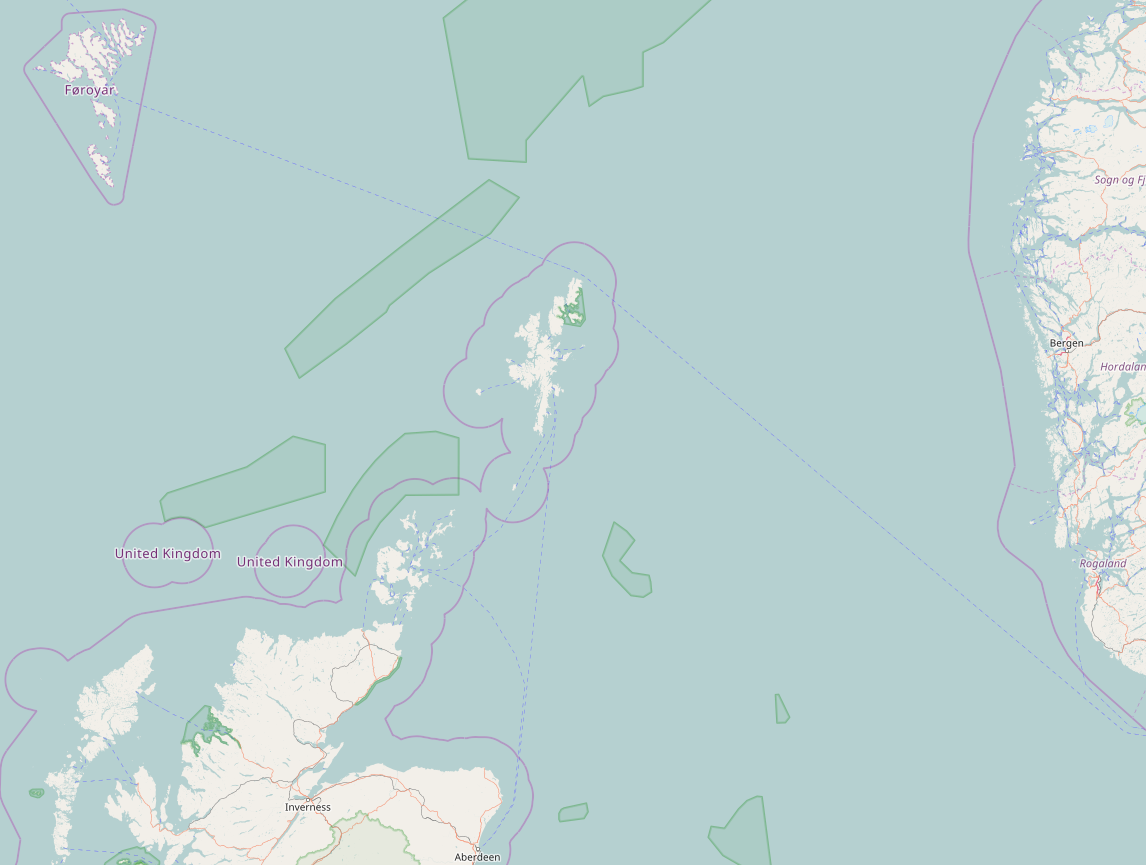
\includegraphics{figure/shetlandcontext}
\caption[Shetland's location in the North Sea]{Shetland's location in the North Sea, showing the territorial waters of the United Kingdom, Norway and the Faroe Islands as well as ferry links and natural conservation areas. % Distance to Bergen + Aberdeen is 350km
Projection:~Web~Mercator. \textcopyright~\href{http://www.openstreetmap.org/copyright}{OpenStreetMap contributors}, licensed under the \href{http://creativecommons.org/licenses/by-sa/2.0/}{Creative Commons Attribution-ShareAlike 2.0 license (CC BY-SA)}.}
% 200dpi=1:5000000 (ferries and marine areas rendered)
% 150dpi=1:7500000
% convert -density 150 -units pixelsperinch in.png out.png
\label{fig:shetlandcontext}
\end{figure}

\begin{figure}
% width=412.56497pt height=629.82918pt
% 6 lines: 0.1925378, 7 lines: 0.1865378
%./remap.py -x ling-Shetland.xml --scale 600910 --width 0.1449794 --height 0.1915378 -o /home/kevin/thesis/questionnaire/figure/shetland.pdf
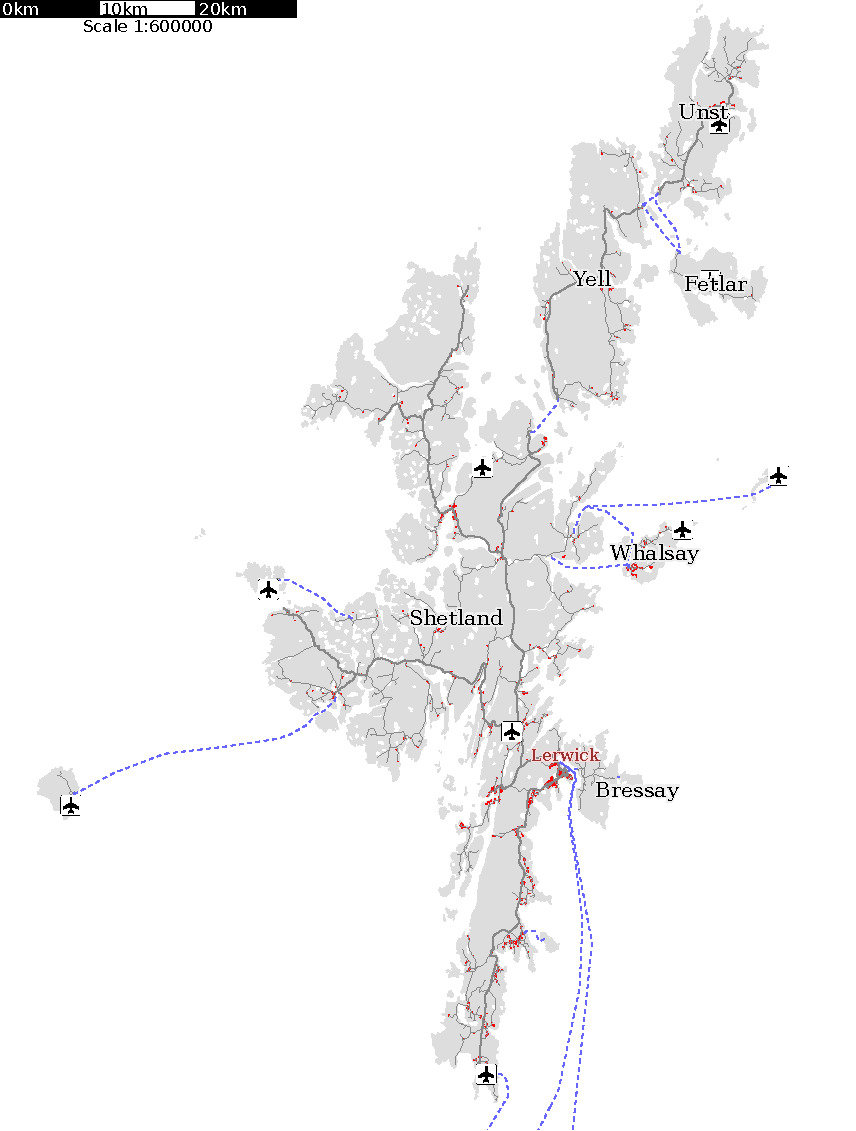
\includegraphics{figure/shetland}
\caption[Detail of the Shetland archipelago]{Detail of the Shetland archipelago showing paved roads, ferry routes, airports and areas of human residence~(in~red). Ferry connections to the Scottish mainland leave from the capital town of Lerwick, also the largest settlement. Regular flights to several Scottish airports as well as Bergen~(Norway) depart from Sumburgh Airport at the Southern tip of the main island, with many more airfields for local planes scattered across the archipelago. Projection:~orthographic, centered on 60.345\textdegree N and 1.4\textdegree W. Map data~\textcopyright~OpenStreetMap contributors.}
\label{fig:shetland}
\end{figure}

Due to its insular location and sustained contact with North Germanic languages~\citep{Jamieson2016}, Shetland Scots has retained many linguistic features typical of Germanic languages that the varieties of English and Scots on the British mainland have long lost. Some examples which will be evident in the questionnaire examples below are the relatively rich verbal inflection, as well as the maintenance of a number distinction in the second person pronoun \emph{du}~(cognate with Middle English \emph{thou}). The features under investigation in this study are also of the historically conservative kind, namely the inversion of the verb position in several syntactic contexts, all of which occur alongside the emergence of periphrastic \emph{do} (or `do-support').
While for most areas of England the change away from the historically original verb-initial constructions~\citep[see][for a more detailed analysis]{Jamieson2015} can be dated to the period from 1500-1700~\citep{Ellegard1953,Kroch1989do}, the homologous change in Shetland Scots has only been unfolding over the course of the 20th century~\citep{Jonas2002}. % Millar2007 p.76
The three related changes currently ongoing in Shetland which we investigate in the current work are as follows:

\begin{itemize}
\item verb positioning in imperatives, which is changing from a raised verb (surface realisation \texttt{VSO}) to Standard English \texttt{SVO} structure. An example in Shetland Scots would be ``Mak du dy ain denner!'' vs. ``Du mak dy ain denner!'', with the latter (incoming) variant akin to Standard English syntax, i.e.~`You~(sg.) make your~(sg.) own dinner!'

\item yes/no question syntax: change from a main verb-initial to a `periphrastic do' structure, e.g. from ``Kens du Sarah?'' to ``Does du ken Sarah?'', with `ken' being the Scots lexeme for `to know'.

\item wh question syntax: change from plain \texttt{WhVSO} with a fronted main verb to a `periphrastic do' structure, i.e. \texttt{Wh-`do'-SVO}. An example of the two constructions would be old ``Whit gae du him?'' to ``Whit did du gie him?'', with `gie'/`gae' the Scots equivalents of Standard English `give'/`gave'.
\end{itemize}

In all three cases, usage of the incoming variants is already common. The two question variables are more advanced, with younger speakers almost categorically using the incoming variants~(with the exception of a few lexically specific items, see \citealt{Jamieson2015}).
% see also a current assessment of acceptability in 
So while the changes are in a sense nearing completion, all members of the speech community are still exposed to both outgoing and incoming variants due to their being used frequently by older speakers.

\subsection{Methodology}\label{sec:questionnaire}

To quantify people's explicit knowledge about ongoing language changes we adapted a self-evaluation method originally used to investigate the perception of phonetic changes by \citet{Labov1966} and \citet{Trudgill1972}, who asked speakers to report their relative usage of several phonetic variables. We refined the methodology, so that every sociolinguistic variable under investigation was covered by a one page questionnaire eliciting speakers' estimates of their own usage, as well as that of other social groups, alongside other (folk-)linguistic beliefs about the linguistic variants themselves\footnote{The complete materials of the paper-based questionnaire can be found in Appendix~\ref{app:questionnaire}.}. At the top of each questionnaire page, the two competing syntactic variants were introduced in the following way:

\begin{framed}
\begin{center}
You are probably familiar with these two ways of asking somebody to do something:\\
``\emph{Mak du dy ain denner!''\hspace{3cm}``Du mak dy ain denner!''}
\end{center}
\end{framed}

The order of the two variants was randomised between individuals, in the above example the outgoing variant is on the left, the incoming one (akin to Standard English ``You make your own dinner!'') on the right. The dialectal spelling of the example sentences is quasi-standardised on Shetland, and their mixing with the Standard English formulations of the questionnaire is not unusual. The actual questionnaire consisted of the following five questions~(referred to as \emph{Q1} through \emph{Q5} throughout the text) which were intended to probe different aspects of people's explicit knowledge about the changes in question:

% How much do you use either of these variants? \begin{likert}\begin{tabular}{ x x x x x } $\square$ & $\square$ & $\square$ & $\square$ & $\square$ \\ I use only `Mak~du..' & I use more `Mak~du..' & I use both equally & I use more `Du~mak..' & I use only `Du~mak..' \end{tabular}\end{likert}

\begin{description}
\item[Question 1:] ``How much do you use either of these variants?'' \hfill \\ This explicit question regarding speakers' own frequency of use could be answered on a 5-point scale, with the options labelled `I use only~(variant 1)', `I use mostly~(variant 1)', `I use both equally', `I use mostly~(variant 2)' and `I use only~(variant 2)', with the order of the two variants matching those of their initial presentation at the top of the page. % This information can be correlated with grammaticality judgments
\item[Question 2:] ``How much do you think are people around you using either of the variants?'' \hfill \\ This question could again be answered on a 5-point scale with options `People use only~(variant 1/2)/mostly~(variant 1/2)/both equally'. This question does not just provide information on speakers' perception of their average interlocutors' frequency of use, but the \emph{relative difference} between the answers to questions 1 and 2 can potentially provide information on whether speakers think of themselves as being `ahead' or `behind' the curve of a particular change relative to their speech community. % (but see results)
\item[Question 3:] ``Which of the two variants do you think is \emph{older}?'' \hfill \\ This (intentionally vague) question is intended to get at speakers' beliefs or connotations regarding the `age' of the competing variants, without drawing explicit attention to the fact that the variable is in fact changing. The three possible answers were `(variant~1) is older', `(variant~2) is older' and `People have always used both', with the order of the two variants randomised.
\item[Questions 4+5:] ``How much do you think \emph{younger/older speakers} use either of the variants?'' \hfill \\ The final two questions tap into speakers' awareness of the apparent time development of a change, with the same 5-point options as above: `Younger/older speakers use only~(variant 1/2)/mostly~(variant 1/2)/both equally'. The order of the two questions was randomised between individuals.
\end{description}

Data collection proceeded in three stages: first, to pilot the methodology, 8~participants were asked to complete the paper version of the questionnaire on site in Shetland in January 2015. The pilot questionnaire consisted of just two sociolinguistic variables with the following example sentences:

\begin{enumerate}
\item verb positioning in imperatives: \emph{Mak du dy ain denner!} vs. \emph{Du mak dy ain denner!}, with the latter (incoming) variant akin to Standard English syntax, i.e.~`You~(sg.) make your~(sg.) own dinner!'
\item negation marking: \emph{He didna go} vs. \emph{He didnoo go} -- this sociolinguistic variable is not undergoing change and was added as a control, with `didna' being the negation variant used categorically in most of Shetland, set against the `didnoo' variant which is categorical only on the island of Whalsay to the East of Shetland's main island~(see Figure~\ref{fig:shetland}). With a population of around 1,000 and close links to the mainland, we expected the local `didnoo' variant (as well as its geographical patterning) to be known to all Shetland locals, an assumption that was borne out by several explicit references to the the variants' distribution by locals during data collection. %, this variable is related to the negation via \emph{na} vs. \emph{no} in mainland Scots).
\end{enumerate}

Following the successful pilot, 16 more participants were asked to complete an extended 4-page version of the questionnaire which covered two further variables:

\begin{enumerate}
\setcounter{enumi}{2}
\item yes/no question syntax: \emph{Kens du Sarah?} vs. \emph{Does du ken Sarah?}, i.e. ``Do you~(sg.) know Sarah?'', with `ken' being the Scots lexeme for `to know'
\item wh question syntax: \emph{Whit gae du him?} vs. \emph{Whit did du gie him?}, the latter again akin to Modern English syntax but with the Scots lexical items for Standard English `what' and `give'.
\end{enumerate}

These first 24 participants were part of a balanced sample matched for binary gender, age, and geographic location within Shetland. All participants grew up in and were currently living in rural locations in Shetland~(i.e.~outside the island's main town, Lerwick). Participants had on average spent 3.7 years living away from Shetland, typically for higher education, work or training purposes. In all cases, the questionnaire was administered as an exit-questionnaire following a $\approx40$~minute task which involved providing grammaticality judgments for a large number of examples of the changing variables in question as well as fillers, which was carried out in pairs~(see~\citealt{Jamieson2015} for a full description of the methodology and analysis of results). % with the researcher being a Shetland local

Finally, we created an identical online version of the 4-variable questionnaire which was advertised via email and social networks. The online questionnaire was self-contained (i.e.~not preceded by the grammaticality judgment task) and provided us with a convenience sample of another 53 participants from all over Shetland, who completed the questionnaire in April 2015\footnote{The online version of the questionnaire is still available for reference at \url{http://spellout.net/ibexexps/kstadler/shetland/experiment.html}.}.
%Apart from their age, gender and current geographical location we also collected information on all participants' occupation, where in Shetland they grew up, any extended times they spent outside the isles, as well as the origin of their parents.

\subsection{Hypotheses \& predictions}\label{sec:questionnairepredictions}

Based on previous research on both the specific syntactic changes under investigation as well as sociolinguistic knowledge more generally, we can derive several predictions about what effects we might expect so see \emph{a priori}.

Regarding differences between the sociolinguistic variables, prior work on verb inversion in Shetland as well as the results derived from the acceptability judgments reported in \citet{Jamieson2015} suggests that the two question variables should pattern differently from the imperatives. The change in question syntax is more advanced, with younger speaker using the incoming question variants almost exclusively. Across the population, we would therefore expect generally higher incoming variant usage for those two variables, as opposed to still relatively mixed usage of the two imperative variants. This general pattern should be observable to different degrees across all of our questions related to usage rates, i.e.~all questions but Q3.

If our informants are indeed aware of the ongoing changes and their directionality, this should be evident in their responses to questions 3 through~5. Here, all three changing variables under investigation should pattern differently from the stable negation variable which acts as our control: since this variable is not undergoing change, it provides us with a baseline for responses to explicit questions about variant age when variable usage is really patterned geographically rather than temporally. % (as far as we can tell none of the studies of sociophonetic knowledge about age reported results from non-changing baseline phonemic distinctions)

In terms of between-participant differences, we can test a number of hypotheses that are implicit in much contemporary sociolinguistic research: because many studies of sound changes in progress have found there to be a significant effect of gender (typically with females leading a change), it has been argued that, primarily due to their position in Western societies, women might be more sensitive to linguistic cues~(\citealt{Trudgill1972}, but see~\citealt{Eckert1989,Labov1990}). While the studies of automatic implicit sociophonetic knowledge discussed above have not revealed any effect of gender, \citet{Carrera-Sabate2014} showed that % based on explicit elicitation
young females were more explicitly aware of an ongoing sound change in the Lleidatà dialect of Catalan. Although no gender differences have been reported for the current syntactic changes in Shetland, neither in production nor in terms of grammatical acceptability~\citep{Jamieson2015}, we can still assess the claim that female speakers might be more sensitive or aware of ongoing changes.

Another interesting question regarding between-speaker differences pertains to how the sociolinguistic knowledge of age patterning might differ between participants of different ages. For example, in her experiment \citet{Drager2011} found an effect of listener \emph{age}, where only \emph{older} participants' perception of vowels that were currently undergoing a chain shift were affected by the perceived age of the speaker whose tokens they were asked to classify. In other words, older speakers were actively compensating more strongly for the manipulated age difference, with younger speakers exhibiting less sociophonetic sensitivity, at least in the sense that they were not actively employing their knowledge of ongoing changes in the classification task. Although we should consider the possibility that the age of our participants will affect their sociolinguistic knowledge of the variables under investigation in this work, it is not possible to derive a straightforward prediction regarding the presence or direction of an effect from the literature. While age effects are also attested in the large body of empirical research on language \emph{attitudes}~\citep{Giles2004}, it is not immediately obvious how and whether the \emph{qualitative} evaluation of innovations (often assumed to be primarily negative, see e.g.~\citealt{Labov2001,Tagliamonte2012}) corresponds to the \emph{quantitative} evaluation and perception of changes, with currently no conclusive results regarding the effect of age on the latter. % We will return to the question of research methodology below.

\section{Results}

Pooling together the data from the paper-based and online questionnaires, the total number of responses was~$N=77$ for the imperative~(\texttt{imp}) and negation~(\texttt{neg}) variables, and~$N=69$ for the yes/no question~(\texttt{ynq}) as well as wh question~(\texttt{whq}) syntax. Both the locally collected and online samples had a similar age distribution, with participants ranging from 18 to 73 years, with a median age of 32.

%round(mean(subset(participants, condition=="online")$age))/round(mean(subset(participants, condition=="paper")$age)), median age median(subset(participants, condition=="online")$age)/r median(subset(participants, condition=="paper")$age)



\begin{figure}[htbp]

{\centering \includegraphics[width=\maxwidth]{figure/questionnairelocation-1} 

}

\caption[Origin of questionnaire participants within Shetland, by condition]{Origin of questionnaire participants within Shetland, by condition~(online convenience sample vs. paper-based controlled sample)}\label{fig:questionnairelocation}
\end{figure}



In terms of the geographical location of our participants there was a bigger difference between the two samples, as can be seen in Figure~\ref{fig:questionnairelocation}. The balanced sample explicitly excluded speakers originally from Shetland's capital Lerwick, home to 7,500 of the islands' total population of 23,000. The Scots vernacular of Lerwick is undergoing a more rapid change towards Standard Scottish English~(SSE) forms than rural variants~\citep{Sundkvist2011}, a development that can be attributed to the larger influx of speakers of other English varieties due to the capital's role as a hub for offshore oil drilling in the surrounding sea.
% For example, the outgoing verb-initial constructions for questions are not attested even in older speakers from Lerwick~(Durham, p.c.).
The convenience sample on the other hand naturally includes a large proportion of Lerwick respondents. However, when it comes to their questionnaire responses, we did not find the Lerwick participants to pattern differently from the rest of the population for any of the questions.
%Even though we collected some information on the socio-economic status of our participants (in particular their profession), this data is of a qualitative nature and will therefore not be used in our statistical models.
%We will go through the results question by question.

Also, despite the fact that we might have expected the on-site participants to be more aware or sensitive to the questionnaire based on the preceding 40~minute acceptability judgment task on related syntactic variables, the type of data collection (paper-based on site vs. online) did not come out as a significant predictor in any of the statistical models reported below.

% TODO correlation between per-individual responses to the three variables?

\subsection{Assessing the reliability of subjective usage judgments}\label{sec:judgmentcorrelation}

Before we turn to the actual data analysis, we have to address a central issue of our methodology, namely the type of data collected and its reliability. While questionnaires are still one of the standard tools employed in dialectological research, explicit questions about language use have fallen into disfavour in the quantitative sociolinguistic tradition. One reason for this is that lay-people's subjective evaluation of linguistic forms is traditionally not regarded as a reliable indicator of usage, as overt evaluations are often assumed to reflect the participants' qualitative sociolinguistic attitudes rather than people's actual quantitative usage~(Labov, Trudgill, inter alia).
%With the topic of language attitudes established as a research area in its own right, in combination with
In combination with the increased availability of speech and text data analysis technology over the past few decades, the relevance of subjective data on language use outside dedicated areas of research such as language attitudes has all but disappeared.
There has, however, been a recent resurgence in interest in the beliefs that non-linguists have about language variation, bridging the two fields with its own set of research methodologies often referred to as \emph{perceptual dialectology}~\citep{Montgomery2011}. % to which the current work can also be attributed.
Rather than completely discarding the opinions of laypersons on the topic of language, this approach raises a number of own research questions regarding how naive speakers' `folk beliefs' about language are related to language use as studied by linguists~\citep{Preston1996}.

It is in this domain that broadly sociolinguistic approaches come closer to the methodologies still most frequently used to study syntax and syntactic variation, in particular by means of \emph{grammaticality judgments} which have over the years been replaced by more gradual \emph{acceptability judgments} provided by naive native speakers rather than linguistic researchers themselves~\citep{Cornips2005}.
% http://web.stanford.edu/group/cslipublications/cslipublications/HPSG/2013/miller.pdf
Based on this continuum of related research methods based on explicit linguistic opinions expressed by speakers, there is also an increasing amount of literature on the question of actual usage is reflected in acceptability judgments and processing preferences~\citep{Sorace2005,Featherston2005} as well as attitudinal data~\citep[see e.g.][]{Maegaard2013,Durham2014}.
In order to better understand the nature of the estimated usage levels obtained through our present methodology it is therefore insightful to cross-validate the results with other measures.
% here are some pointers I got off Jim Donaldson that one could possibly go into: Miller, Arregui et al. 2006 (The Recycling Hypothesis), Gibson and Thomas 1999 (perceiving ungrammatical sentences as grammatical), Hofmeister et al. 2014 Processing effects in linguistic judgment data, Keller 2001 Gradience in grammar, Manning 2003 Probabilistic syntax, Sorace and Keller 2005 Gradience in linguistic data)
%One concern is thus that the estimated usage rates reported, particularly those concerning the speakers' \emph{own} usage, might not be representative.
% TODO general sociolinguistic focus on phonetics/data critique?
%really the question of reliability is not the only reason for the abandonment of questionnaires, it coincided nicely with a focus on high-frequency phonetic variables and the increasing availability of recording devices
%One obvious concern regarding our methodology, which draws the participants' explicit attention to the changing variables in question, is how indicative the responses are of speakers' actual usage.
While we have no quantitative production data available for the three changing syntactic variables in question which are all very low in frequency,
we can, however, compare the relative usage rates against the grammatical acceptability judgments which were collected independently for the 24~participants during the first, on site phase of data collection~(see~\citealt{Jamieson2015}). %reported by the same participants.
If the novel methodology presented here is indeed reliable, we should expect good correlation between the two measures.

Despite the fact that both grammaticality judgments and usage rate estimates were gathered through explicit elicitation, there are two big differences between the two types of data: firstly, the usage rate estimates draw explicit attention to the type of speaker that it is envisaged to be representative of, i.e.~the speaker themselves, the `average' interlocutor in their community, or a `younger' or `older' speaker specifically. This framing focusses explicitly on the variants' use in a specific context, while the acceptability judgment draws the informants' attention primarily to the linguistic variant itself.
In this way, a quantitative acceptability judgment does not distinguish in a principled manner between utterances that the informant would use in their own production, and what they would accept (or expect) from some of their interlocutors, but never actually produce themselves.

The second difference is that the usage rates as collected here capture the \emph{relative} usage of the two competing variants of a sociolinguistic variable by directly contrasting the two equivalent forms of a single example sentence. The acceptability judgments on the other hand express the \emph{absolute} acceptability of an individual example sentence on a 7-point Likert scale, without speaking directly to the \emph{relative} usage of the two competing variants.

In order to assess the reliability of our usage estimates by correlating it with the acceptability judgment data, we first need to transform the two measures to comparable scales, keeping in mind those differences. The basic idea here is to convert the absolute judgments per variant into relative ratings per variable, by comparing the per-variant ratings of the incoming and outgoing realisations of the same example sentences. Transforming the acceptability judgments to relative scores can be done in several different ways and boils down to three decisions. While none of the choices turned out to have a strong effect on the results, it is worth discussing them to get an idea of how a methodology based around acceptability judgments can be related to the present questionnaire methodology.

The first question regards exactly \emph{which} acceptability judgments should be correlated with the usage estimates. The acceptability judgment data collected by~\citet{Jamieson2015} is more abundant: each of the 24~informants provided judgments for a total of 49~example sentences across the three changing variables, covering 17~different verb types, and some of the verbs were chosen because they are known to exhibit strong lexical effects that affect the choice of syntactic construction. The two principled ways to limit the lexical effects on the acceptability measures are, on one hand, to only correlate the judgments for those sentences where the verbs match those used in the respective example sentences from the questionnaire or, alternatively, to wash out lexical effects by taking the average acceptability score over all verbs used in the acceptability judgment task. Both approaches turn out to result in almost identical correlation coefficients, and even the inclusion of all individual lexical items leads to a highly significant (if~lower) correlation coefficient.

The second decision relates to how the two acceptability judgments for the two competing variants should be converted into one measure capturing their relative acceptability, akin to the direct juxtaposition of the ``which variant do you use more'' measure employed by the questionnaire. The two most straightforward ways to combine them into one measure is by taking the difference between the ratings for the incoming and the outgoing variant, either by subtraction (absolute difference in acceptability) or division (relative difference in acceptability). %\footnote{While division is in principle not a legal operation for ordinal responses, acceptability judgments collected on a Likert scale are frequently treated as numeric responses, and subjected to parametric statistical tests, see e.g.~\citet{TODO}.}.
Both approaches produce a numeric scale with a neutral centre point occupied by pairs of judgments where the incoming and outgoing variants were rated to be equally acceptable~($0$ for the absolute difference by subtraction, and $1$ for the relative difference by division). In terms of the relative ranking of pairs with differing judgments the two scales only differ marginally, as can be seen in Figure~\ref{fig:judgments} below, where it is relatively easy to identify the matching pairs of datapoints between the two graphs based on their y-axis position.\footnote{The main difference between the two different ways to convert the acceptability judgments concerns the resolution of the resulting scale: pairwise subtraction of the 7 possible ranks of the ordinal acceptability judgments yields a total of~13 possible relative ratings, while the division method results in up to~35 theoretically possible values, and consequently fewer ties. The impact of choosing either of the two approaches on the resulting correlation coefficients is still only marginal, and our results are not highly sensitive to either choice, as can be seen below.} %The coefficients derived from both calculations are reported in the results below.

Having transformed the absolute acceptability judgments to a relative acceptability scale, there is still a third decision to be made, namely which of the usage estimate ratings it should be correlated with. The separate questions in the questionnaire gathered data regarding different speaker groups, including the informants themselves as well as several idealised interlocutor groups. Intuitively, we would expect people's acceptability judgments to reflect their own probability of producing the respective variants, and it is indeed only their self-usage estimates that yield a significant correlation with the derived relative acceptability scores.

The relationship between the reported relative self-usage rates and both the absolute and relative difference in acceptability reported by the 24~participants in the paper condition are shown in Figure~\ref{fig:judgments}. Due to the large number of ties along the 5-point ordinal scale of the questionnaire we chose Kendall's $\tau_B$ to calculate the correlation between the two measures. We found the strongest correlation between informants' self-usage estimates and the relative difference of their acceptability judgments by division, with $\tau_B=0.22207$. This correlation is significant at $p<.01$, as determined using the \texttt{pvrank} R package which provides p-value calculation for rank order correlation tests accounting for ties~\citep{pvrank1.1}. % TODO could also do clme(self ~ judgment, random=id, data=da) ??

\begin{figure}[htbp]

{\centering \includegraphics[width=\maxwidth]{figure/judgments-1} 

}

\caption[Correlation between the 24 informants' reported self-usage rate of the two variants for the three changing variables and the relative acceptability derived from the average acceptability judgments]{Correlation between the 24 informants' reported self-usage rate of the two variants for the three changing variables~(x-axis, jittered) and the relative acceptability derived from the average acceptability judgments (y-axis), for two ways of calculating the relative preference of the variants: (a)~\emph{absolute} difference in acceptability, calculated by subtracting the rating of the outgoing variant from the incoming one (b)~\emph{relative} difference of the incoming vs. outgoing ratings, calculated by division. The mid-points of the two relative acceptability scales~(where two competing variants are judged as equally acceptable) are indicated by dashed lines.}\label{fig:judgments}
\end{figure}



%(TODO could delve into comparing the two data types a bit more here, e.g. by looking at the marginal distributions of the acceptability vs. usage estimate data and see how the difference between them might capture facts about how far the change has already progressed?)

%The distribution of the relative acceptability judgments (plotted along the y-axis) is insightful: for the more advanced changes to the two question variables all but one variant pairing yielded a higher acceptability of the incoming question syntax, as can be seen from their placement above the central `equal acceptability' line.

%Those participants who found the incoming variants more acceptable also rated themselves as using them more often.

Having established that the subjective responses that make up our data set pattern closely with an independent measure of use in the form of acceptability judgments,
%do not merely reflect their sociolinguistic attitudes 
% speakers' actual usage, at least as far as we can derive from their
we can now turn to analysing our participants' responses, and the patterns found therein.

\subsection{Self-estimates of own usage}
\label{sec:selfresponses}

The first measure elicited from our participants was an estimate of their own usage levels for each of the linguistic variables in question.
The overall data, split by sociolinguistic variable and informant age, is shown in Figure~\ref{fig:selfresponses}. The first impression is that the response distribution is highly uneven, with the majority of responses falling onto the three categories of our 5-point-scale that indicate at least 50\% usage of the incoming variants.\footnote{Since the control variable exhibits stable variation, there is no `incoming' or `outgoing' variant in this sense. Instead, we have coded the more frequently used (i.e. geographically more widespread) variant as the `incoming' one.}

\begin{figure}[htbp]

{\centering \includegraphics[width=\maxwidth]{figure/selfresponses-1} 

}

\caption[Distribution of informant age per reported level of own usage for the three changing variables as well as the stable, geographically conditioned control]{Distribution of informant age per reported level of own usage for the three changing variables as well as the stable, geographically conditioned control. The five response levels correspond to the five possible responses described in Section~\ref{sec:questionnaire}, ranging from the leftmost `I only use the incoming variant' to `I only use the outgoing variant' at the very right.}\label{fig:selfresponses}
\end{figure}





As expected, the self-reports on the stable negation variable are patterned by the informants' geographical location, with the only four informants indicating categorical usage of the more localised variant all originating from the isle of Whalsay. In contrast, responses for the three changing variables appear to reflect differences in usage patterns in \emph{apparent time}, the familiar phenomenon where the language use of younger speakers is found to be more \emph{advanced}, i.e.~they exhibit higher usage rates of the new, incoming variants~\citep{Wagner2012theory}.
%In other words, if speakers are reporting their own usage accurately, we should expect individual responses to be predicted by the speakers' age, with younger speakers reporting higher usage levels of the incoming variants. The distribution of ages per response suggests that there might be such an effect:
While the mean age of respondents tends to decrease for higher reported usage of the incoming variants for the three changing variables, the same is not true for the stable control variable.
% For the three changing variables, however, the mean age of the respondents tends to decrease for responses reporting higher levels of the incoming variant.

% in unit age on the outcome distribution.
%This first result captures the fact that the change in verb position in imperatives is indeed lagging behind the two question variables.

%This conclusion receives independent support from the grammaticality judgments elicited from the first 24~participants, which exhibited high acceptability for both imperative variants, in contrast to comparatively lower acceptability ratings for the outgoing question forms\footnote{For an extended discussion of how the usage rate estimates correlate to acceptability judgments, see section~\ref{sec:judgmentcorrelation}.}.
% FIXME gotta select proper subset of judgment stimuli that matches the awareness questionnaires in terms of verb arity etc.?

To test our hypotheses we used ordered logistic regression, an extension of logistic regression that allows for more than two (ordered) response categories. We fit a number of models of increasing complexity using R's \texttt{ordinal} package~\citep{ordinal2015}, with participant as a random effect. %\footnote{Linear mixed effects regression models with the response variable coded as numeric rather than ordinal yields the same picture.}
% TODO and we performed model comparison using log-likelihood tests~\citep{Barr2013}.
The results from these models are shown in Table~\ref{table:selfresponsesmodelordinal}: the four coefficients at the very bottom of the table, present for all models, are equivalent to the \emph{intercept} in (generalised) linear models, only that ordinal regression requires $n-1$ intercepts to capture the baseline distribution of responses across the $n$ response levels. The coefficients above it capture the inferred effect of the various predictor variables on the outcome distribution of self-evaluation responses along the 5-point ordinal scale. Ordered logistic models can be read like any regression model, except that the intercepts are given as \emph{log odds ratios}, and the coefficients $\beta_i$ as \emph{difference in log odds} per unit change in the predictor variable. In other words, with every unit change in the predictor, the relative odds ratio of responding in a lower vs. a higher category as given by the intercepts is multiplied by $\exp(\beta_i)$.

Looking at the succession of models in Table~\ref{table:selfresponsesmodelordinal} as well as the pairwise model comparison between them in Table~\ref{table:selfresponsesmodelordinalcomparison}, we first find a strong effect of the type of sociolinguistic variable (model~1): in comparison to the stable negation variant for which the majority of speakers reported using only the `incoming' variant, the imperatives~(\texttt{varimp}) exhibit significantly more responses in the center of the 5-point scale, with the two question types~(\texttt{varynq}, \texttt{varwhq}) falling somewhere in between. While we find no evidence for an effect of informant age across all variables~(model~2) there appears to be an effect of gender, with females being more likely to report increased use of the majority variants~(model~3). % This effect is not particular to the changing variables, adding an interaction is not significant
% TODO include the intermediate age*stable+var (but with no gender) model as well?
When taking into account differences between the different sociolinguistic variables, we do find evidence for an effect of age for the changing variables only.
Rather than using the \texttt{var} term, a 4-level factor that distinguishes all sociolinguistic variables covered by the questionnaire, model~4 adds an interaction between the age coefficient and the \emph{type} of sociolinguistic variable, with the binary \texttt{stable} factor opposing the three changing variables against the stable negation variable.
Even though the model \emph{comparison} between models~3 and~4 in Table~\ref{table:selfresponsesmodelordinalcomparison} is not significant, 
the model coefficient $\beta_{age}=\ensuremath{-0.028}$ means that the relative probability of responding in a higher category is multiplied by $\exp(\ensuremath{-0.028})=0.972$ for every year that a participant is \emph{older}. This is equivalent to their probability of reporting a relatively higher usage level of the incoming variant \emph{decreasing} slightly (by about 2.8\%). The coefficient of the \texttt{age:stable} interaction term, which is of a similar amplitude but in the opposite direction~($\beta_{age:stable}=0.039$), implies that this effect of age is effectively cancelled out for the stable control variable.


% Table created by stargazer v.5.2 by Marek Hlavac, Harvard University. E-mail: hlavac at fas.harvard.edu
% Date and time: Thu, Aug 18, 2016 - 13:49:00
\begin{table}[htbp] \centering 
  \caption{Ordered logistic regression model (coefficients and standard errors) of participants' own usage estimates.} 
  \label{table:selfresponsesmodelordinal} 
\begin{tabular}{@{\extracolsep{5pt}}lccccc} 
\\[-1.8ex]\hline 
\hline \\[-1.8ex] 
\\[-1.8ex] & (1) & (2) & (3) & (4) & (5)\\ 
\hline \\[-1.8ex] 
 age &  & $-$0.019 & $-$0.020 & $-$0.028$^{*}$ & $-$0.019 \\ 
  &  & (0.011) & (0.011) & (0.012) & (0.016) \\ 
  stable &  &  &  & 1.031 &  \\ 
  &  &  &  & (0.901) &  \\ 
  gendermale &  &  & $-$0.788$^{*}$ & $-$0.817$^{*}$ & $-$0.838$^{*}$ \\ 
  &  &  & (0.359) & (0.365) & (0.370) \\ 
  age:varynq &  &  &  &  & $-$0.005 \\ 
  &  &  &  &  & (0.023) \\ 
  age:varwhq &  &  &  &  & $-$0.033 \\ 
  &  &  &  &  & (0.023) \\ 
  age:varneg &  &  &  &  & 0.030 \\ 
  &  &  &  &  & (0.024) \\ 
  varynq & 1.909$^{***}$ & 1.874$^{***}$ & 1.864$^{***}$ & 1.865$^{***}$ & 2.052$^{*}$ \\ 
  & (0.372) & (0.372) & (0.372) & (0.374) & (0.960) \\ 
  varwhq & 1.770$^{***}$ & 1.736$^{***}$ & 1.732$^{***}$ & 1.733$^{***}$ & 2.997$^{**}$ \\ 
  & (0.365) & (0.365) & (0.366) & (0.367) & (0.985) \\ 
  varneg & 2.558$^{***}$ & 2.575$^{***}$ & 2.567$^{***}$ &  & 1.403 \\ 
  & (0.414) & (0.414) & (0.415) &  & (0.979) \\ 
  age:stable &  &  &  & 0.039 &  \\ 
  &  &  &  & (0.021) &  \\ 
  only out\textbar more out & $-$3.204$^{***}$ & $-$3.965$^{***}$ & $-$4.261$^{***}$ & $-$4.648$^{***}$ & $-$4.290$^{***}$ \\ 
  & (0.450) & (0.651) & (0.665) & (0.711) & (0.801) \\ 
  more out\textbar both & $-$2.282$^{***}$ & $-$3.036$^{***}$ & $-$3.336$^{***}$ & $-$3.713$^{***}$ & $-$3.366$^{***}$ \\ 
  & (0.348) & (0.579) & (0.595) & (0.642) & (0.738) \\ 
  both\textbar more in & $-$0.996$^{***}$ & $-$1.747$^{**}$ & $-$2.051$^{***}$ & $-$2.407$^{***}$ & $-$2.065$^{**}$ \\ 
  & (0.280) & (0.532) & (0.547) & (0.590) & (0.692) \\ 
  more in\textbar only in & 0.884$^{**}$ & 0.132 & $-$0.172 & $-$0.493 & $-$0.135 \\ 
  & (0.274) & (0.512) & (0.522) & (0.558) & (0.669) \\ 
 \hline \\[-1.8ex] 
\textit{Note:}  & \multicolumn{5}{r}{$^{*}$p$<$0.05; $^{**}$p$<$0.01; $^{***}$p$<$0.001} \\ 
\end{tabular} 
\end{table} 

% Table created by stargazer v.5.2 by Marek Hlavac, Harvard University. E-mail: hlavac at fas.harvard.edu
% Date and time: Thu, Aug 18, 2016 - 13:49:01
\begin{table}[!htbp] \centering 
  \caption{Pairwise comparison of the models in Table~\ref{table:selfresponsesmodelordinal}.} 
  \label{table:selfresponsesmodelordinalcomparison} 
\begin{tabular}{@{\extracolsep{5pt}} cccccccc} 
\\[-1.8ex]\hline 
\hline \\[-1.8ex] 
 & Model & Res. df & -2LL & Test & df & LR & P(\textgreater Chi) \\ 
\hline \\[-1.8ex] 
(0) & 1 & $287$ & $606.566$ &  & $$ & $$ &  \\ 
(1) & var & $284$ & $551.283$ & 0 vs 1 & $3$ & $55.282$ & \textless  .001 \\ 
(2) & age + var & $283$ & $548.353$ & 1 vs 2 & $1$ & $2.930$ & .087 \\ 
(3) & age + gender + var & $282$ & $543.518$ & 2 vs 3 & $1$ & $4.835$ & .028 \\ 
(4) & age:stable + gender + var & $281$ & $540.054$ & 3 vs 4 & $1$ & $3.464$ & .063 \\ 
(5) & age:var + gender & $279$ & $537.920$ & 4 vs 5 & $2$ & $2.134$ & .344 \\ 
\hline \\[-1.8ex] 
\end{tabular} 
\end{table} 

\begin{figure}[!ht]

{\centering \subfloat[Empirical distribution of the self-reported usage levels for the three changing variables, with the participants split into two age groups ($\le32$ years, $N=39$; $>32$ years, $N=38$). The younger the speaker, the more likely they are to report higher usage of the incoming variant.\label{fig:selfresponsesprediction1}]{\includegraphics[width=\maxwidth]{figure/selfresponsesprediction-1} }
\subfloat[Prediction of response distributions of ordered logistic model (4) from Table~\ref{table:selfresponsesmodelordinal} for the mean ages of the two age groups plotted above.\label{fig:selfresponsesprediction2}]{\includegraphics[width=\maxwidth]{figure/selfresponsesprediction-2} }

}

\caption[Comparison of empirical own usage reports and corresponding model prediction]{Comparison of empirical own usage reports and corresponding model prediction.}\label{fig:selfresponsesprediction}
\end{figure}



Finally, fitting a model with separate interaction terms for each of the four variables (by substituting the \texttt{age:stable} term with \texttt{age:var}, model~5) does not improve the model fit significantly, indicating that the presence of the age effect is mostly explained by whether the sociolinguistic variable is undergoing change or not.

To help visualise the effect of age and aid in interpreting the log odd ratio coefficients, the empirical responses by age as well as the corresponding predictions made by the ordered logistic models are shown in Figure~\ref{fig:selfresponsesprediction}. For this purpose we split the responses we collected into two evenly sized age groups, %($age <= 32, N=39$; $age > 32, N=38$)
and the distribution of responses per age group and sociolinguistic variable is shown in Figure~\ref{fig:selfresponsesprediction}a: despite differing baseline distributions (with imperatives generally exhibiting a flatter distribution), we can see the general trend of increasing incoming variant usage for younger speakers. The predictions made by model~4 for the different variables and a typical member of each of the two age groups are plotted underneath in Figure~\ref{fig:selfresponsesprediction}b, showing good agreement with the empirical data.

\subsection{`Other people' usage estimates}
\label{sec:otherresponses}

When it comes to reporting on the linguistic usage levels of other individuals in their speech community, the overall pattern of responses is similar to the self-usage estimates, but with an added central tendency or edge-avoiding effect in the responses, as can be seen in Figure~\ref{fig:otherresponses}. This presumably stems from the fact that, when imagining an `average' individual, the informants will model this on the \emph{population average}, which, given any amount of within- or between-individual variation, is almost necessarily non-categorical.

Again, we performed ordered logistic regression models with participant as a random effect, reported in Tables~\ref{table:otherresponsesmodel} and~\ref{table:otherresponsesmodelcomparison}.
In contrast to the self-usage reports, we find no effect of age for any of the variables~(models~1+2). Instead, the models reveal that the only significant predictors of the reported usage levels are the type of sociolinguistic variable~(model~3) as well as the participant's gender, with females again estimating slightly \emph{higher} usage of the incoming variant in the community~(model~4). Importantly we find no significant interaction between the type of variable and any of the other predictors, i.e. the effect of gender again pertains to all four variables, and not just the changing ones~(model~5).


% Table created by stargazer v.5.2 by Marek Hlavac, Harvard University. E-mail: hlavac at fas.harvard.edu
% Date and time: Thu, Aug 25, 2016 - 14:00:23
\begin{table}[htbp] \centering 
  \caption{Ordered logistic regression model (coefficients and standard errors) predicting participants' answers to the question ``How much do you think are people around you using either of the variants?''} 
  \label{table:otherresponsesmodel} 
\begin{tabular}{@{\extracolsep{5pt}}lccccc} 
\\[-1.8ex]\hline 
\hline \\[-1.8ex] 
\\[-1.8ex] & (1) & (2) & (3) & (4) & (5)\\ 
\hline \\[-1.8ex] 
 age & 0.005 & $-$0.002 &  &  &  \\ 
  & (0.011) & (0.012) &  &  &  \\ 
  stable &  & $-$0.560 &  &  &  \\ 
  &  & (0.771) &  &  &  \\ 
  age:stable &  & 0.023 &  &  &  \\ 
  &  & (0.019) &  &  &  \\ 
  varynq &  &  & 1.750$^{***}$ & 1.749$^{***}$ & 1.751$^{***}$ \\ 
  &  &  & (0.404) & (0.404) & (0.404) \\ 
  varwhq &  &  & 1.888$^{***}$ & 1.883$^{***}$ & 1.884$^{***}$ \\ 
  &  &  & (0.410) & (0.410) & (0.410) \\ 
  varneg &  &  & 1.491$^{***}$ & 1.487$^{***}$ & 1.222$^{**}$ \\ 
  &  &  & (0.387) & (0.388) & (0.450) \\ 
  gendermale &  &  &  & $-$0.832$^{*}$ & $-$1.019$^{*}$ \\ 
  &  &  &  & (0.368) & (0.406) \\ 
  gendermale:stable &  &  &  &  & 0.743 \\ 
  &  &  &  &  & (0.654) \\ 
  only out\textbar more out & $-$5.821$^{***}$ & $-$6.045$^{***}$ & $-$5.294$^{***}$ & $-$5.615$^{***}$ & $-$5.717$^{***}$ \\ 
  & (1.092) & (1.120) & (1.037) & (1.053) & (1.059) \\ 
  more out\textbar both & $-$3.465$^{***}$ & $-$3.686$^{***}$ & $-$2.829$^{***}$ & $-$3.141$^{***}$ & $-$3.232$^{***}$ \\ 
  & (0.537) & (0.591) & (0.408) & (0.440) & (0.451) \\ 
  both\textbar more in & $-$1.659$^{***}$ & $-$1.873$^{***}$ & $-$0.835$^{**}$ & $-$1.136$^{***}$ & $-$1.215$^{***}$ \\ 
  & (0.446) & (0.509) & (0.289) & (0.322) & (0.332) \\ 
  more in\textbar only in & 2.471$^{***}$ & 2.300$^{***}$ & 3.825$^{***}$ & 3.519$^{***}$ & 3.464$^{***}$ \\ 
  & (0.469) & (0.516) & (0.419) & (0.421) & (0.424) \\ 
 \hline \\[-1.8ex] 
\textit{Note:}  & \multicolumn{5}{r}{$^{*}$p$<$0.05; $^{**}$p$<$0.01; $^{***}$p$<$0.001} \\ 
\end{tabular} 
\end{table} 

%\afterpage{%
\begin{figure}[htbp]\RawFloats

{\centering \subfloat[Overall distribution of reported \emph{own} usage, per sociolinguistic variable.\label{fig:otherresponses1}]{\includegraphics[width=\maxwidth]{figure/otherresponses-1} }
\subfloat[Responses to the question ``How much do you think are people around you using either of the variants?''. While the distribution of responses to the imperative question is again consistently flatter than for the other responses, in comparison to the self-usage estimates shown in (a) there is a clear shift away from both of the extreme response options, indicating that individuals perceive the population average to be variable rather than categorical.\label{fig:otherresponses2}]{\includegraphics[width=\maxwidth]{figure/otherresponses-2} }

}

\caption[Comparison of own vs. community-level usage estimates by binary gender]{Comparison of own vs. community-level usage estimates by binary gender.}\label{fig:otherresponses}

% Table created by stargazer v.5.2 by Marek Hlavac, Harvard University. E-mail: hlavac at fas.harvard.edu
% Date and time: Thu, Aug 25, 2016 - 14:00:24
%\begin{table}[!htbp] \centering 
  \captionof{table}{Pairwise comparison of the models in Table~\ref{table:otherresponsesmodel}.} 
  \label{table:otherresponsesmodelcomparison} 
\begin{tabular}{@{\extracolsep{5pt}} cccccccc} 
\\[-1.8ex]\hline 
\hline \\[-1.8ex] 
 & Model & Res. df & -2LL & Test & df & LR & P(\textgreater Chi) \\ 
\hline \\[-1.8ex] 
(0) & 1 & $287$ & $507.936$ &  & $$ & $$ &  \\ 
(1) & age & $286$ & $507.702$ & 0 vs 1 & $1$ & $0.234$ & .628 \\ 
(2) & age:stable & $284$ & $505.271$ & 1 vs 2 & $2$ & $2.431$ & .297 \\ 
(3) & var & $284$ & $478.018$ & 1 vs 3 & $2$ & $29.684$ & \textless  .001 \\ 
(4) & var + gender & $283$ & $472.928$ & 3 vs 4 & $1$ & $5.089$ & .024 \\ 
(5) & var + gender:stable & $282$ & $471.625$ & 4 vs 5 & $1$ & $1.303$ & .254 \\ 
\hline \\[-1.8ex] 
\end{tabular} 
%\end{table} 
\end{figure}
%}
\FloatBarrier

The data from the first two questions implicitly contains another piece of information, namely where the speakers regard their own variable usage to be relative to the community-level. We measure this by looking at the number of ordinal categories along the 5-point scale that the self-usage response \emph{differs} from the reported community-level usage, and subtracting their ordinal ranks. In this representation of the relative difference, positive numbers indicate that a speaker reported a relatively higher usage of the incoming variant for themselves than for the community, and vice versa.
% this representation collapses different responses, e.g. +3 can mean 'older only out, younger more in' as well as 'older mostly out, younger only in', 0 could be 'older usage = younger usage' for any of the 5 usage levels

If we look at the distribution of this measure in Figure~\ref{fig:selfdiff}, we see that the participants' age is a good predictor of this difference between themselves and the community. %The binary partitioning suggested by conditional inference shows that the majority of under-58-year-olds regard themselves as `ahead' of their community in terms of using the incoming variants, whereas those over 58 are most likely to report being level with the community~(
Ordinal logistic regression models paralleling those fit to the self-usage reports in Table~\ref{table:selfresponsesmodelordinalcomparison} above confirm this picture: as can be seen in Tables~\ref{table:selfdiffmodel} and~\ref{table:selfdiffmodelcomparison}, the most parsimonious model predicts the difference between individuals' reported own and community usage based on the type of sociolinguistic variable as well as the informant's age. Although the effect of age is again greater for the changing variables~(compare models~2 and~3), the models indicate no significant difference between the stable as opposed to any of the changing variables~(models~3+4).

\begin{figure}[htbp]

{\centering \includegraphics[width=\maxwidth]{figure/selfdiff-1} 

}

\caption[Relative difference in number of ordinal categories between participants' reported \emph{own} vs community usage levels of the competing variants, by sociolinguistic variable and age group]{Relative difference in number of ordinal categories between participants' reported \emph{own} vs community usage levels of the competing variants, by sociolinguistic variable and age group. Positive numbers indicate that a speaker reported a higher usage of the incoming variant for themselves than for the community, and vice versa. While the 5-point response scale allows for differences of up to $\pm4$, no speaker indicated their own usage to be more than two ordinal categories away from the community level. Younger speakers are more likely to perceive themselves to be ahead of the community level usage~(more red), while older speakers are most likely to report their usage to be level with the community~(white) or behind~(blue).}\label{fig:selfdiff}
\end{figure}


% Table created by stargazer v.5.2 by Marek Hlavac, Harvard University. E-mail: hlavac at fas.harvard.edu
% Date and time: Thu, Aug 18, 2016 - 14:11:56
\begin{table}[htbp] \centering 
  \caption{Ordered logistic regression model (coefficients and standard errors) of the relative difference between participants' reported own and community-level usage.} 
  \label{table:selfdiffmodel} 
\begin{tabular}{@{\extracolsep{5pt}}lcccc} 
\\[-1.8ex]\hline 
\hline \\[-1.8ex] 
\\[-1.8ex] & (1) & (2) & (3) & (4)\\ 
\hline \\[-1.8ex] 
 age &  & $-$0.022$^{*}$ & $-$0.027$^{*}$ & $-$0.023 \\ 
  &  & (0.010) & (0.011) & (0.016) \\ 
  stable &  &  & 0.633 &  \\ 
  &  &  & (0.745) &  \\ 
  varynq & 0.883$^{**}$ & 0.850$^{*}$ & 0.841$^{*}$ & 1.481 \\ 
  & (0.337) & (0.336) & (0.337) & (0.879) \\ 
  varwhq & 0.677$^{*}$ & 0.636 & 0.624 & 0.494 \\ 
  & (0.336) & (0.336) & (0.337) & (0.881) \\ 
  varneg & 1.305$^{***}$ & 1.322$^{***}$ &  & 0.796 \\ 
  & (0.343) & (0.343) &  & (0.858) \\ 
  age:stable &  &  & 0.018 &  \\ 
  &  &  & (0.017) &  \\ 
  age:varynq &  &  &  & $-$0.017 \\ 
  &  &  &  & (0.022) \\ 
  age:varwhq &  &  &  & 0.004 \\ 
  &  &  &  & (0.022) \\ 
  age:varneg &  &  &  & 0.013 \\ 
  &  &  &  & (0.020) \\ 
  -2\textbar -1 & $-$3.312$^{***}$ & $-$4.156$^{***}$ & $-$4.377$^{***}$ & $-$4.223$^{***}$ \\ 
  & (0.422) & (0.583) & (0.627) & (0.759) \\ 
  -1\textbar 0 & $-$1.934$^{***}$ & $-$2.788$^{***}$ & $-$3.000$^{***}$ & $-$2.847$^{***}$ \\ 
  & (0.307) & (0.504) & (0.549) & (0.692) \\ 
  0\textbar +1 & 0.432 & $-$0.426 & $-$0.618 & $-$0.461 \\ 
  & (0.269) & (0.462) & (0.500) & (0.652) \\ 
  +1\textbar +2 & 4.180$^{***}$ & 3.324$^{***}$ & 3.129$^{***}$ & 3.302$^{***}$ \\ 
  & (0.414) & (0.535) & (0.568) & (0.715) \\ 
 \hline \\[-1.8ex] 
\textit{Note:}  & \multicolumn{4}{r}{$^{*}$p$<$0.05; $^{**}$p$<$0.01; $^{***}$p$<$0.001} \\ 
\end{tabular} 
\end{table} 

% Table created by stargazer v.5.2 by Marek Hlavac, Harvard University. E-mail: hlavac at fas.harvard.edu
% Date and time: Thu, Aug 18, 2016 - 14:11:56
\begin{table}[!htbp] \centering 
  \caption{Pairwise comparison of the models in Table~\ref{table:selfdiffmodel}.} 
  \label{table:selfdiffmodelcomparison} 
\begin{tabular}{@{\extracolsep{5pt}} cccccccc} 
\\[-1.8ex]\hline 
\hline \\[-1.8ex] 
 & Model & Res. df & -2LL & Test & df & LR & P(\textgreater Chi) \\ 
\hline \\[-1.8ex] 
(0) & 1 & $287$ & $657.692$ &  & $$ & $$ &  \\ 
(1) & var & $284$ & $642.109$ & 0 vs 1 & $3$ & $15.583$ & .001 \\ 
(2) & age + var & $283$ & $637.137$ & 1 vs 2 & $1$ & $4.972$ & .026 \\ 
(3) & age:stable + var & $282$ & $636.056$ & 2 vs 3 & $1$ & $1.081$ & .298 \\ 
(4) & age:var & $280$ & $635.065$ & 3 vs 4 & $2$ & $0.990$ & .609 \\ 
\hline \\[-1.8ex] 
\end{tabular} 
\end{table} 


\subsection{Beliefs about the age of competing linguistic variants}
\label{sec:oldervar}

%Before explicitly drawing attention to the fact that the linguistic variables are changing~(and that this might be reflected in apparent time differences),
The third question of the questionnaire aimed at eliciting the speakers' beliefs about the variants by explicitly asking which they thought was the `older' of the two, with `people have always used both' given as a neutral third option. As can be seen in Figure~\ref{fig:variantage}, people reliably identify the outgoing variant as the `older' one for the three changing variables. For the stable negation variable results are more mixed, but many also report the less widespread `didnoo' variant as being older.

The ordered logistic regression models reported in Tables~\ref{table:variantagemodel} and~\ref{table:variantagemodelcomparison} show that, while participants generally tend to report the less frequent variants to be older, they are more likely to do so for the three changing variables~(model~3). There is also again a significant interaction between the type of variable and the age of the informant: older informants are more likely to identify the outgoing variant as the `older' one, but again only for the sociolinguistic variables that are changing~(models~2-5). Beyond the split between the stable and changing variables, there was no significant difference between the individual variables~(models~3-6), and we also found no evidence for any effect of gender. % not reported

%While the consistency of individual responses indicate that the community shares common beliefs about the \emph{directionality} of these changes, this result does not speak to the source of these beliefs. We will return to this issue in the Discussion.

\begin{figure}[htbp]

{\centering \includegraphics[width=\maxwidth]{figure/variantage-1} 

}

\caption[Distribution of responses to the question ``Which of the two variants do you think is \emph{older}?'', split by sociolinguistic variable and age of the informant]{Distribution of responses to the question ``Which of the two variants do you think is \emph{older}?'', split by sociolinguistic variable and age of the informant. In comparison to the stable negation variant, where about half of the people considered the geographically more limited (minority) variant `didnoo' to be older, the response distribution was more extreme for the three changing variables. Here, around 80\% of respondents report the outgoing forms (which are already the minority forms) to be older, with even fewer answers falling on the majority variant as well as the ``people have always used both'' option.}\label{fig:variantage}
\end{figure}


% Table created by stargazer v.5.2 by Marek Hlavac, Harvard University. E-mail: hlavac at fas.harvard.edu
% Date and time: Thu, Aug 18, 2016 - 13:20:50
\begin{table}[htbp] \centering 
  \caption{Ordered logistic regression model (coefficients and standard errors) of responses to the question ``Which of the two variants do you think is \emph{older}?''.} 
  \label{table:variantagemodel} 
\begin{tabular}{@{\extracolsep{5pt}}lcccccc} 
\\[-1.8ex]\hline 
\hline \\[-1.8ex] 
\\[-1.8ex] & (1) & (2) & (3) & (4) & (5) & (6)\\ 
\hline \\[-1.8ex] 
 gendermale & 0.494 &  &  &  &  &  \\ 
  & (0.373) &  &  &  &  &  \\ 
  age &  & 0.007 &  &  & $-$0.016 & $-$0.016 \\ 
  &  & (0.012) &  &  & (0.015) & (0.015) \\ 
  stable &  &  & 1.404$^{***}$ &  & $-$0.751 & $-$0.617 \\ 
  &  &  & (0.308) &  & (0.789) & (0.843) \\ 
  varynq &  &  &  & 0.373 &  & 0.320 \\ 
  &  &  &  & (0.435) &  & (0.438) \\ 
  varwhq &  &  &  & 0.080 &  & 0.028 \\ 
  &  &  &  & (0.440) &  & (0.444) \\ 
  varneg &  &  &  & 1.557$^{***}$ &  &  \\ 
  &  &  &  & (0.401) &  &  \\ 
  age:stable &  &  &  &  & 0.058$^{**}$ & 0.057$^{**}$ \\ 
  &  &  &  &  & (0.020) & (0.020) \\ 
  outgoing older\textbar always both & 1.232$^{***}$ & 1.315$^{**}$ & 1.531$^{***}$ & 1.685$^{***}$ & 0.963 & 1.103 \\ 
  & (0.249) & (0.490) & (0.248) & (0.359) & (0.604) & (0.678) \\ 
  always both\textbar incoming older & 3.251$^{***}$ & 3.332$^{***}$ & 3.727$^{***}$ & 3.891$^{***}$ & 3.254$^{***}$ & 3.403$^{***}$ \\ 
  & (0.355) & (0.556) & (0.384) & (0.472) & (0.674) & (0.747) \\ 
 \hline \\[-1.8ex] 
\textit{Note:}  & \multicolumn{6}{r}{$^{*}$p$<$0.05; $^{**}$p$<$0.01; $^{***}$p$<$0.001} \\ 
\end{tabular} 
\end{table} 

% Table created by stargazer v.5.2 by Marek Hlavac, Harvard University. E-mail: hlavac at fas.harvard.edu
% Date and time: Thu, Aug 18, 2016 - 13:20:51
\begin{table}[!htbp] \centering 
  \caption{Pairwise comparison of the models in Table~\ref{table:variantagemodel}.} 
  \label{table:variantagemodelcomparison} 
\begin{tabular}{@{\extracolsep{5pt}} cccccccc} 
\\[-1.8ex]\hline 
\hline \\[-1.8ex] 
 & Model & Res. df & -2LL & Test & df & LR & P(\textgreater Chi) \\ 
\hline \\[-1.8ex] 
(0) & 1 & $288$ & $434.312$ &  & $$ & $$ &  \\ 
(1) & gender & $287$ & $432.539$ & 0 vs 1 & $1$ & $1.773$ & .183 \\ 
(2) & age & $287$ & $433.952$ & 0 vs 2 & $1$ & $0.360$ & .549 \\ 
(3) & stable & $287$ & $412.654$ & 0 vs 3 & $1$ & $21.658$ & \textless  .001 \\ 
(4) & var & $285$ & $411.839$ & 3 vs 4 & $2$ & $0.815$ & .665 \\ 
(5) & age:stable & $285$ & $403.374$ & 3 vs 5 & $2$ & $9.279$ & .01 \\ 
(6) & age:stable + var & $283$ & $402.723$ & 5 vs 6 & $2$ & $0.652$ & .722 \\ 
\hline \\[-1.8ex] 
\end{tabular} 
\end{table} 


\subsection{Perception of apparent time differences}
\label{sec:apparenttime}

The final pair of questions, which ask for the participants' impression of the relative usage level of the two competing variants by `younger' and `older' speakers was aimed at helping us to determine whether individuals can perceive and report apparent time differences in categorical variables. As can be seen in Figure~\ref{fig:apparenttime}, speakers consistently report higher usage of the majority variants among younger speakers but, surprisingly, this effect is present across all sociolinguistic variables, including the stable control.
%Interestingly, hardly anyone attributed higher usage of the majority variant to older speakers, so that $0$ works as a `hard edge'
While there appears to be a general trend to attribute the usage of minority variants (whether outgoing or just geographically limited) to older speakers, the ordinal logistic regression model~2 in Tables~\ref{table:apparenttimemodel} and~\ref{table:apparenttimemodelcomparison} shows that the effect is significantly stronger for the three changing variables, but with no significant differences between them~(compare models~3+4).
In contrast to the responses to question~3, the age of our informants does not appear to have a systematic effect on how they perceive apparent time differences for any of the variables under investigation~(models~1+4).
% TODO report responses to individual q4+5 answers: only type of variable makes a difference!

\begin{figure}[htbp]

{\centering \includegraphics[width=\maxwidth]{figure/apparenttime-1} 

}

\caption[Relative difference between the reported usage of the two variants between `older' and `younger' speakers, for each of the four variables]{Relative difference between the reported usage of the two variants between `older' and `younger' speakers, for each of the four variables. The relative difference indicates the number of ordinal categories that separates an individuals' responses for the two age groups along the 5-point scale, where positive numbers (in shades of red) correspond to reporting higher usage of the majority variant among younger speakers, and vice versa. The most extreme points of the scale at $\pm4$ correspond to reporting the `older' and `younger' speakers to be categorical users of opposing variants, the mid-point at $0$ to reporting the same usage levels for both.}\label{fig:apparenttime}
\end{figure}


% Table created by stargazer v.5.2 by Marek Hlavac, Harvard University. E-mail: hlavac at fas.harvard.edu
% Date and time: Mon, Aug 22, 2016 - 13:45:08
\begin{table}[htbp] \centering 
  \caption[Ordered logistic regression model (coefficients and standard errors) of the relative difference in individuals' estimates for `younger' and `older' speaker groups in number of ordinal categories]{Ordered logistic regression model (coefficients and standard errors) of the relative difference in individuals' estimates for `younger' and `older' speaker groups in number of ordinal categories, a proxy for perceived apparent time differences. Raw data is shown in Figure~\ref{fig:apparenttime}.} 
  \label{table:apparenttimemodel} 
\begin{tabular}{@{\extracolsep{5pt}}lccccc} 
\\[-1.8ex]\hline 
\hline \\[-1.8ex] 
\\[-1.8ex] & (1) & (2) & (3) & (4) & (5)\\ 
\hline \\[-1.8ex] 
 age & $-$0.011 &  &  & $-$0.005 &  \\ 
  & (0.008) &  &  & (0.010) &  \\ 
  stable &  & $-$1.535$^{***}$ &  & $-$0.804 & $-$1.215$^{***}$ \\ 
  &  & (0.266) &  & (0.653) & (0.274) \\ 
  varynq &  &  & $-$0.432 &  &  \\ 
  &  &  & (0.310) &  &  \\ 
  varwhq &  &  & 0.052 &  &  \\ 
  &  &  & (0.312) &  &  \\ 
  varneg &  &  & $-$1.674$^{***}$ &  &  \\ 
  &  &  & (0.322) &  &  \\ 
  age:stable &  &  &  & $-$0.020 &  \\ 
  &  &  &  & (0.016) &  \\ 
  oldervaralways both &  &  &  &  & $-$1.325$^{***}$ \\ 
  &  &  &  &  & (0.317) \\ 
  oldervarincoming older &  &  &  &  & $-$2.316$^{***}$ \\ 
  &  &  &  &  & (0.575) \\ 
  -2\textbar -1 & $-$5.109$^{***}$ & $-$5.445$^{***}$ & $-$5.590$^{***}$ & $-$5.697$^{***}$ & $-$6.176$^{***}$ \\ 
  & (0.673) & (0.620) & (0.648) & (0.730) & (0.661) \\ 
  -1\textbar 0 & $-$4.108$^{***}$ & $-$4.435$^{***}$ & $-$4.581$^{***}$ & $-$4.680$^{***}$ & $-$5.121$^{***}$ \\ 
  & (0.494) & (0.417) & (0.457) & (0.567) & (0.466) \\ 
  0\textbar +1 & $-$1.801$^{***}$ & $-$1.970$^{***}$ & $-$2.114$^{***}$ & $-$2.171$^{***}$ & $-$2.454$^{***}$ \\ 
  & (0.354) & (0.215) & (0.284) & (0.432) & (0.254) \\ 
  +1\textbar +2 & $-$0.328 & $-$0.301 & $-$0.432 & $-$0.490 & $-$0.636$^{***}$ \\ 
  & (0.327) & (0.164) & (0.242) & (0.402) & (0.189) \\ 
  +2\textbar +3 & 1.690$^{***}$ & 1.914$^{***}$ & 1.810$^{***}$ & 1.726$^{***}$ & 1.730$^{***}$ \\ 
  & (0.354) & (0.220) & (0.275) & (0.424) & (0.230) \\ 
  +3\textbar +4 & 5.397$^{***}$ & 5.689$^{***}$ & 5.591$^{***}$ & 5.500$^{***}$ & 5.572$^{***}$ \\ 
  & (1.049) & (1.013) & (1.026) & (1.077) & (1.016) \\ 
 \hline \\[-1.8ex] 
\textit{Note:}  & \multicolumn{5}{r}{$^{*}$p$<$0.05; $^{**}$p$<$0.01; $^{***}$p$<$0.001} \\ 
\end{tabular} 
\end{table} 

% Table created by stargazer v.5.2 by Marek Hlavac, Harvard University. E-mail: hlavac at fas.harvard.edu
% Date and time: Mon, Aug 22, 2016 - 13:45:09
\begin{table}[!htbp] \centering 
  \caption{Pairwise comparison of the models in Table~\ref{table:apparenttimemodel}.} 
  \label{table:apparenttimemodelcomparison} 
\begin{tabular}{@{\extracolsep{5pt}} cccccccc} 
\\[-1.8ex]\hline 
\hline \\[-1.8ex] 
 & Model & Res. df & -2LL & Test & df & LR & P(\textgreater Chi) \\ 
\hline \\[-1.8ex] 
(0) & 1 & $284$ & $829.962$ &  & $$ & $$ &  \\ 
(1) & age & $283$ & $828.119$ & 0 vs 1 & $1$ & $1.842$ & .175 \\ 
(2) & stable & $283$ & $794.396$ & 0 vs 2 & $1$ & $35.565$ & \textless  .001 \\ 
(3) & var & $281$ & $791.493$ & 2 vs 3 & $2$ & $2.904$ & .234 \\ 
(4) & age:stable & $281$ & $791.456$ & 2 vs 4 & $2$ & $2.941$ & .23 \\ 
(5) & stable + oldervar & $281$ & $764.235$ & 2 vs 5 & $2$ & $30.161$ & \textless  .001 \\ 
\hline \\[-1.8ex] 
\end{tabular} 
\end{table} 


While this might suggest that individuals can accurately perceive and report on apparent age differences in changing categorical variables, we cannot straightforwardly jump to this conclusion. Model~5 shows that our participants' responses to question~3 (i.e. their reported belief about which if any of the competing variants is `older') %, and in particular the `wrong' classification of the incoming variant as the `older' one
is a significant predictor of how far they reported younger speakers to be `ahead' or `behind' in their relative usage of the incoming variant.
So while all results presented so far show that individuals are clearly able to (correctly) report on the directionality of the changes under investigation, the exact \emph{source} of this metalinguistic knowledge is still in question. We turn to this issue in our discussion.

\section{Discussion}

Having presented the questionnaire data as well as statistical models of the individual responses, we now turn our attention to the particular research questions and predicted effects discussed in Section~\ref{sec:questionnairepredictions}.

\subsection{Identifying the source of awareness of ongoing changes}
\label{sec:questionorder}

The main goal of our research was to quantify if and to what degree individuals are aware of and able to report on the direction of ongoing changes in their community, with a particular eye on whether individuals are sensitive to differences in `apparent time', i.e.~the traditionally more advanced usage of incoming variants among younger speakers.
While the results presented in Sections~\ref{sec:oldervar} and~\ref{sec:apparenttime} indicate that people have accurate knowledge about ongoing changes, our data does not allow us to give a definite answer regarding the \emph{source} of this knowledge.
In principle, beliefs could be based on any or all of (a)~meta-linguistic commentary or other connotations of variants being archaic, (b)~impressions of the change in \emph{real time}, i.e.~awareness of changing speech patterns that accumulate throughout a speaker's lifetime, or (c)~apparent time differences in variable usage across age groups.
%The present challenge is to identify, if possible, the source of
The questionnaire was designed with these different sources of knowledge in mind. In particular, while questions 4+5 tapped into speakers knowledge about apparent time differences between speakers, the responses to question~3 offer a more general window into individuals' folk-linguistic beliefs about the `age' or novelty of the competing variants.

As already indicated above, the two measures turned out to be highly correlated: model~(5) in Table~\ref{table:apparenttimemodel} showed the folk-linguistic belief about variant age is itself a good predictor of individuals' perceived apparent time differences, as derived from questions 4+5.
%Conversely, we can expand the models predicting people's reports about the perceived age of variant (model 4 from Tables~\ref{table:variantagemodel} and~\ref{table:variantagemodelcomparison}) by adding the perceived apparent time difference that we can extrapolate from questions 4+5.
Importantly, the converse is also true: Tables~\ref{table:oldervarq3model} and~\ref{table:oldervarq3modelcomparison} report expanded models of individuals' responses to question~3, showing that the apparent time differences gathered from the responses to questions 4+5 are a good predictor of the responses to question~3. The number of ordinal categories between the reported `older' and `younger' usage levels~(coded as a continous variable~\texttt{apparentdiffN}) is in fact a better predictor of the participants' folk-linguistic belief than whether the variable is actually changing or not~(compare models~1 and~2).
What the models do not suggest, however, is that folk-linguistic beliefs are based on perceived apparent time differences alone~(model~3). Other predictors remain significant, in particular the interaction between informant age and the type of sociolinguistic variable reported earlier in Section~\ref{sec:oldervar}. Even when the participants' impression of apparent age differences is taken into account, there is still a significant effect of informant age on their responses, with older participants less likely to report the less frequent variant as older for the stable control variable only~(compare models~4 and~5).
%The effect does not completely outweigh the role of variable however, instead the effect of these two factors appears to be cumulative.

Based on these results it remains an open question whether people might have inferred their answer to question~3 independently from a perceived apparent time difference, or if participants felt led to answer questions~4 and 5 in a way that would post-hoc justify their earlier response, which was itself based on other~(socio-indexical) knowledge.
In order to understand the different sources of socio-indexical knowledge that might be at play here, it is insightful to take a closer look at the responses to our control variable.


% Table created by stargazer v.5.2 by Marek Hlavac, Harvard University. E-mail: hlavac at fas.harvard.edu
% Date and time: Thu, Aug 18, 2016 - 14:45:13
\begin{table}[htbp] \centering 
  \caption[Extension of the ordered logistic regression model in Table~\ref{table:variantagemodel}, adding individuals' perceived apparent time difference as an additional predictor]{Extension of the ordered logistic regression model in Table~\ref{table:variantagemodel}, adding individuals' perceived apparent time difference as an additional predictor for their responses to the question ``Which of the two variants do you think is older?''.} 
  \label{table:oldervarq3model} 
\begin{tabular}{@{\extracolsep{5pt}}lccccc} 
\\[-1.8ex]\hline 
\hline \\[-1.8ex] 
\\[-1.8ex] & (1) & (2) & (3) & (4) & (5)\\ 
\hline \\[-1.8ex] 
 age &  &  &  & 0.002 & $-$0.020 \\ 
  &  &  &  & (0.013) & (0.016) \\ 
  stable & 1.404$^{***}$ &  & 0.816$^{*}$ & 0.815$^{*}$ & $-$1.229 \\ 
  & (0.308) &  & (0.332) & (0.332) & (0.841) \\ 
  apparentdiffN &  & $-$1.124$^{***}$ & $-$1.002$^{***}$ & $-$1.001$^{***}$ & $-$0.984$^{***}$ \\ 
  &  & (0.185) & (0.190) & (0.190) & (0.190) \\ 
  age:stable &  &  &  &  & 0.055$^{**}$ \\ 
  &  &  &  &  & (0.021) \\ 
  outgoing older\textbar always both & 1.531$^{***}$ & $-$0.234 & 0.176 & 0.264 & $-$0.504 \\ 
  & (0.248) & (0.280) & (0.332) & (0.618) & (0.684) \\ 
  always both\textbar incoming older & 3.727$^{***}$ & 2.199$^{***}$ & 2.675$^{***}$ & 2.764$^{***}$ & 2.075$^{**}$ \\ 
  & (0.384) & (0.348) & (0.415) & (0.678) & (0.726) \\ 
 \hline \\[-1.8ex] 
\textit{Note:}  & \multicolumn{5}{r}{$^{*}$p$<$0.05; $^{**}$p$<$0.01; $^{***}$p$<$0.001} \\ 
\end{tabular} 
\end{table} 

% Table created by stargazer v.5.2 by Marek Hlavac, Harvard University. E-mail: hlavac at fas.harvard.edu
% Date and time: Thu, Aug 18, 2016 - 14:45:14
\begin{table}[!htbp] \centering 
  \caption{Pairwise comparison of the models in Table~\ref{table:oldervarq3model}.} 
  \label{table:oldervarq3modelcomparison} 
\begin{tabular}{@{\extracolsep{5pt}} cccccccc} 
\\[-1.8ex]\hline 
\hline \\[-1.8ex] 
 & Model & Res. df & -2LL & Test & df & LR & P(\textgreater Chi) \\ 
\hline \\[-1.8ex] 
(0) & 1 & $288$ & $434.312$ &  & $$ & $$ &  \\ 
(1) & stable & $287$ & $412.654$ & 0 vs 1 & $1$ & $21.658$ & \textless  .001 \\ 
(2) & apparentdiffN & $287$ & $384.260$ & 0 vs 2 & $1$ & $50.053$ & \textless  .001 \\ 
(3) & stable + apparentdiffN & $286$ & $378.250$ & 2 vs 3 & $1$ & $6.009$ & .014 \\ 
(4) & age + stable + apparentdiffN & $285$ & $378.222$ & 3 vs 4 & $1$ & $0.029$ & .866 \\ 
(5) & age:stable + apparentdiffN & $284$ & $370.925$ & 4 vs 5 & $1$ & $7.297$ & .007 \\ 
\hline \\[-1.8ex] 
\end{tabular} 
\end{table} 


%So while there is strong correlation between the folk-linguistic beliefs and perceived apparent time differences, our analysis suggests that it might not be possible to reduce either of them to the other: in both models other predictors are highly significant, showing that the responses mutual influence explains some, but not all of the effect.

%While we can't derive a definite answer, there is at least some indication that both sources -- apparent time differences and folk-linguistic beliefs -- are at play in answering the respective other question.

%Conversely, the direction of the relative ordinal difference between the reported younger/older speaker usage is also a significant predictor of the answer to the preceding ``Which of the two variants do you think is \emph{older}?'' question~(model 2), with a reported apparent time difference~(i.e.~an ordinal difference~$>0$) predicting increased identification of the outgoing variant as the `older' one.

%One potential way to find out whether the latter is the case is by checking whether the absolute progression of the changes, where the imperatives seem to lag behind a bit, is also evident in the answers about the specific age group questions. The overall pattern of relative apparent age differences does not differ for the questions vs. the imperatives TODO redo this
% i.e.check whether people's young/old responses are better predicted by their self/other responses or by oldervar?



\subsection[Variant age and perceived apparent time differences]{Variant age and perceived apparent time differences: evidence from the control variable}

Some more evidence regarding the primary source of inividuals' knowledge can be glanced from the responses to our control variable. As the distribution of negation variants on Shetland is stable, determined by geography rather than by generational change, we would not expect any information on the history of the two variants to be available to our speakers.
Regarding their answers to the first two questions, the control patterned as expected. Own usage reports were predicted perfectly by geographical location, with all four participants indicating categorical usage of the `noo' variant~(coded as `outgoing' in the Figures) coming from the isle of Whalsay. The estimates of the community-wide usage consequently fell chiefly in the `more incoming' category, with no clear internal patterning of responses along any of the participant variables~(see Figure~\ref{fig:otherresponses}).



%Since age does not affect the reported self-usage levels of the negation variable, and the reported community-level usage is consistent for all variables, there is consequently no effect of age on how much people report to use the negation variants relative to their surrounding community.
When it came to beliefs about the relative age of the two negation variants in question~3 we found that, despite the apparent absence of any evidence for it, almost half of the participants stated that they believed that the geographically limited negation variant was `older' than its more widespread counterpart, as could be seen in Figure~\ref{fig:variantage}.
This result is puzzling: the geographical distribution of the two variants is well-known to Shetland inhabitants, an assumption that was confirmed by the fact that 17~out of 77~participants used the optional comment field to point out that the variable realisation of negation patterned geographically and not by time, the dimension investigated by the questionnaire. %(one participant in the on-site paper-based version of the questionnaire even omitting this question, instead noting the geographical pattern as a side comment).

% TODO mention that apparent time diff is best predictor, but adding age still improves the model significantly~($p=format.p.value(anova(nullmdl, agemdl)[["Pr(>Chisq)"]][-1])$) % TODO include Chisq stats?
%While this result in itself requires explanation, we also observed an additional interaction with age, indicating that the age of the participant affected their beliefs about the stable variables different from the changing ones.
%Fitting a simple ordered logistic regression model to the negation data only confirms a significant effect of age, with older participants \emph{less} likely to identify the localised minority variant as the older one~($p=format.p.value(agemdl$stats["Score P"])$).
%In terms of perceived age of the variants, the only significant age effect is actually with the stable negation variable, where older people are more likely to identify the geographically more widespread `didnoo' variant as being the `older' one~(caveat: that is still only 8 out of 76 people, and those 8 happen to contain relatively older speakers).
%rms::orm(oldervarfreq ~ age+gender+firstvar+firstolder+condition, data=neg)


%A similarly intriguing result can be obtained from the perceived apparent time differences derived from the participants' answers to questions 4+5. 
The distribution of perceived apparent time differences for our control revealed a similarly intriguing result: as the negation variable isn't changing we would have expected the distribution of difference scores to be centered around the zero mark.
While Figure~\ref{fig:apparenttime} showed that identical estimates for the `older' and `younger' speaker groups was indeed the most frequently reported result across all our participants, the overall distribution of responses is skewed towards reporting higher usage of the more widespread variant for younger speakers, with almost no apparent time differences reported in the opposite direction.



This raises the question of why speakers would extrapolate from a geographical pattern to history, or at least to the historical origin of variants. While there is currently no evidence that the relative usage of the more localised negation variant is decreasing~(Jamieson, p.c.), it is imaginable that it shares a few meta-linguistic features with the outgoing variants of the changing variables. As the more `local' variant, it could have gathered connotations of `dialectality' and `authenticity' that are typically associated with older speakers. %~(TODO are there results regarding whether this is generally the case, sociolinguistically? Is there any particular reason to believe this might be true on Shetland?).
This (possibly imagined) prevalent usage among older speakers could in turn give rise to both effects observed in the responses: firstly, it could be regarded to speak to the variant's historical primacy~\citep{Bailey2002}, and secondly, the usage pattern by authentic `older' speakers stands in natural opposition to younger speakers, explaining the reported differences in apparent time, an effect that was possibly amplified by the ordering of questions in the survey.

As it stands, it is not possible for us to identify the exact pathway of these socio-indexical connotations. Does `authenticity' speak to both speaker group differences \emph{and} variant history, or does one affect the other?
While the responses to the changing variables provide evidence that apparent time differences are perceived independently, we can again not rule out that the responses to questions~4+5 were influenced so as to provide a post-hoc justification of the earlier answer regarding the variants' relative age. Conversely, the presence of seemingly non-substantiated beliefs about variant age for the control variable might indicate that, when forced to identify one variant as `older', our participants might attribute historical primacy based on imagined age stratification even when they know that, synchronically, usage is determined by geography alone.

To avoid the same problem and aid in identifying the influence of either type of knowledge, an improved methodology should therefore randomise the order of questions~3~vs.~4+5 between individuals.% and, time allowing, also embed~4+5 in a bigger set of distractor questions.
The two randomisations could then serve as separate conditions:
measuring the effect of first explicitly drawing attention to either linguistic history \emph{or} apparent time differences between participants would allow us to quantify what effect either meta-linguistic dimension has on the other.

%This result could indicate that answers about the age of the variants were based on perceived differences in the apparent time distribution, but it could also be
%Does this mean that we should think of the causality as going from answering apparent time differences to folk-linguistic beliefs about variant age, and not vice versa?

% TODO gotta fit something about the subsets??
%subset(d, firstolder==TRUE)

%Despite the fact that up to this point in the questionnaire we avoided to draw explicit attention to such differences



\subsection{Between-participant differences: age}

Our results revealed several significant effects of the informants' age on their responses: firstly, age is a good predictor for participants' reported self-use of the changing variables, as reported in Section~\ref{sec:selfresponses}. In combination with the fact that age did not seem to affect participants' estimates of the community-level usage,
age is consequently a good predictor for how much the respondents think they are `ahead' or `behind' their estimated community level usage, as measured by the relative difference between people's estimated self and community usage levels~(Section~\ref{sec:otherresponses}). This suggests that individuals can correctly identify where, during an ongoing change, they are positioned relative to the rest of the community.

While \citet{Drager2011} found that older speakers were more sensitive in their automatic compensation for ongoing phonetic changes, we find no such effect for the explicit reports on syntactic variables. For the changing variables, there is no significant effect of informant age on either the perceived `age' of the variants %~(TODO need to fit this model separately, this is not straightforwardly clear from Section~\ref{sec:oldervar})
or the perceived differences in apparent time~(Section~\ref{sec:apparenttime}).%, or on the estimates of how much `younger' and `older' speaker groups use the variants.

\subsection{Between-participant differences: gender}

The only significant effects of binary gender were found in the first two questions, i.e.~the reported `self' as well as `other speakers' usage levels: females tended to report \emph{higher} levels of the incoming variant both for themselves and the population as a whole. This tendency was present across all four sociolinguistic variables, whether changing or not.
The raw data of the responses split by variable and gender is shown in Figure~\ref{fig:genderreports}.

\begin{figure}[htbp]

{\centering \includegraphics[width=\maxwidth]{figure/genderreports-1} 

}

\caption[Raw data for responses regarding self-usage by sociolinguistic variable and binary gender]{Raw data for responses regarding self-usage by sociolinguistic variable and binary gender. For the changing variables, females generally report higher level usage of the incoming majority variants.}\label{fig:genderreports}
\end{figure}



This gender effect does \emph{not} translate to a higher difference between perceived self-usage and perceived community usage, i.e.~females do \emph{not} perceive themselves to be further `ahead' the community than males do, the answers to both questions appear to be shifted in unison. Also, despite an often purported increased sensitivity to linguistic changes among females, neither the identification of the `older' variants~(Section~\ref{sec:oldervar}) nor the strength of the perceived apparent time differences~(Section~\ref{sec:apparenttime}) showed significant effects of participant gender.
%In relation to previous sociolinguistic research which has revealed gender differences where women were often found to be leading linguistic changes has been used to argue that, due to their social position, women are more sensitive to sociolinguistic cues~(Labov, inter alia).

%For the three changing variables pooled together, whether participants correctly report the outgoing variant to be older is not predicted well by any of the participant variables, in particular not by gender or age.

% SELFDIFF thoughts:
% intriguing fact about selfdiff: 50% of people report themselves as being ahead, under 10% as being behind
%counts <- table(subset(d, var!='neg')$selfdiff, factor(subset(d, var!='neg')$var))
%barplot(t(t(counts)/colSums(counts)), legend=rownames(counts), col=cm.colors(5))
% Apart from the effect of age, it is intriguing that very few individuals report themselves to be `behind' the curve for the question types, as opposed to the imperatives. This effect might be a matter of the measure used here: the imperatives, still very much a change in progress, allow for a wider range of putting yourself `relative' to the community usage (on either extreme). Maybe, instead of measuring the absolute difference between selected categories per individual, the relative difference should be measured relative to the distribution of community-level responses?


% people are also VERY consistent in their 'young' reports viz. the earlier 'other people' community average
%plot(party::ctree(young ~ other+loc+age+gender+firstvar+firstolder+condition+var, data=changing))
% the same isn't true for the older speakers, for which the variable remains the only significant predictor
%plot(party::ctree(old ~ other+loc+age+gender+firstvar+firstolder+condition+var, data=changing))
% ordered logistic models of this fail due to many empty cells in the 5x5 table...

% correctly identifying the outgoing variable is a good predictor for rating older speakers as *really* outdated
%plot(party::ctree(olddiff ~ oldervar+loc+age+gender+firstvar+firstolder+condition+var, changing))
% but younger speakers are actually mostly marked as level (could be a combination of ceiling+edge-avoidance??)
%plot(party::ctree(youngdiff ~ oldervar+loc+age+gender+firstvar+firstolder+condition+var, changing))

\section{Summary \& conclusion}

In this work, we presented a new methodology to assess and measure quantitatively whether people can report the direction of currently ongoing changes based on their awareness of the variable usage levels of categorical sociolinguistic variables.
Results from 77 speakers show that people are reliably capable of reporting
apparent time differences within their speech community, as well as provide evaluations of the age of the different linguistic variants that are compatible with the direction of the changes.
Complementing earlier experimental results on individual speakers' use of their implicit knowledge of continuous sound changes, we obtained quantitative evidence for the explicit awareness of changes in three related morphosyntactic variables which are only attested at very low frequencies in everyday speech.
Even though their low frequency means that we have no quantitative production data to compare to, the absolute usage levels reported by our informants reflect what is known about the relative progress of the three changes, indicating that naive individuals can learn about variable usage rates even from very limited data.
%which makes them hard to study quantitatively for linguists -- it means that individuals do not have that much data available to figure out the changes either, and still they seem to be able to do it pretty well!
While it is possible that explicit socio-indexical commentary on the variants could be underlying the shared knowledge about the direction of changes, the quantitative difference in responses between variables as well as the age-stratified distribution of self-usage assessments within variables
suggests that the degree of knowledge about the variants cannot be straightforwardly reduced to qualitative connotations of specific variants as being `older', `more dialectal' etc.

Connecting the present work to related approaches, I briefly discussed the continuum of methodologies that are based on eliciting explicit judgments on language and language use from laypeople.
Our extension of a simple and fast survey method originally employed by \citet{Labov1966} and \citet{Trudgill1972} falls on a spectrum somewhere between current quantitative methods employed in syntactic research and the qualitative approaches to variation pervasive in the study of language attitudes. Our work is best understood as a contribution to the re-emerging field of \emph{perceptual dialectology} dedicated to the study of naive language users' impression of language variation and change. This branch of research embraces the assumption that subjective evaluations, whether qualitative or quantitative, should not be discarded a priori but that they can complement and support evidence collected by other means in important ways.
In Section~\ref{sec:judgmentcorrelation} in particular we showed that subjective reports of relative quantitative usage correlate well with measures derived from grammatical acceptability judgments.
% We investigated how the estimated usage rates that we elicited from participants relate to the other quantitative measure of linguistic evaluation available to us, namely acceptability judgments.

%age vector stuff
In the context of this thesis, the present work represents an empirical contribution to the study of individuals' capacity to detect and monitor ongoing changes in their community.
%Unlike in the case of evolution by self-replication (such as genes/genomes in the traditional view of biological evolution), the fact that linguistic conventions are replicated by external entities (humans) means that they are inherently open to a different set of selection mechanisms than the ones typically associated with evolution.
As argued in Chapter~\ref{ch:review}, the \emph{metalinguistic awareness} of innovations and changes in the individual provides a rich source for social biases which could underlie selection mechanisms at play in language change, such as the momentum-based selection bias presented in the previous chapter.
%idea that the selection of linguistic innovations could be driven 
While we complemented and extended existing work to morphosyntactic, categorical variables of low frequency, the study of individuals' sociolinguistic knowledge is still a new topic that will require much further work, particularly in respect to innovations and changes.

%and some concluding remark about how important meta-linguistic knowledge can potentially be in driving change.

%Humans do not just make use of linguistic conventions, they are also \emph{aware} of their own (and others') usage of specific conventions, as well as how patterns of use differ across space and time. 
%One unique future of human languages is that they even allow one to make \emph{meta-linguistic commentary} on language use, i.e. natural language allows one to \emph{language} about language~\citep{DeBeule2014}.


\chapter{Symmetric selection of asymmetric innovation}%: contextualising momentum
%and the generation of linguistic variants
% interacting pressures of variation and selection
\label{ch:bigpicture}
\chapter[Asymmetric generation of variants]{Competing selection pressures and the generation of linguistic variants}

% This thesis has zoomed in on one particular pressure. The aim of this chapter is to situate the pressure in relation to other mechanisms that are involved in language change, as well as provide theoretical motivations for why momentum could (and should) be relevant for language change research.

\section{Competing motivations in linguistic change}

% From Anderson to Bickel
%\citep{Sundgren2009,Wichmann?}

historical contingency~\citep[p.503]{Labov2001} % Gould?

\section{Language change and replicator-neutrality}

% arbitrariness
% directed variation + directional selection
\citet{Sapir1921}'s `drift': languages do not just diverge when there is social pressure to discriminate, but also have an internal `drive' to change (in place) by themselves (p.160).

\citep[ch.7-12]{Labov2010} on forks in the road etc.

challenging the notion that ``a reliance on chance deprives an account of any real explanatory value" \citep[p.44]{Joseph2013}.

\section{Neutral selection of non-random variation}

% biology: \citep{Gerlee2015}

\section{Modelling the interaction of different pressures}
\label{sec:asymmetricvariation}

%One argument put forward in the previous sections was that, in order to explain asymmetries, it is not necessary to construe the prevalent conventions as having been selected for for that purpose.

In this section I will present a simple model to investigate how a symmetric momentum bias, a selection bias favouring trending conventions whether they are beneficial or deterious, interacts with asymmetric \emph{generation} of variants. The model is an extension of the Markov model of Bayesian Iterated Learning that was analysed in-depth in Section~\ref{sec:realigriffiths}.\index{Markov model}

To recapitulate, \citet{Reali2009} proposed a model of regularisation by Iterated Learning. In their model, a Bayesian learner infers the underlying relative frequencies of several competing variants based on a sample of productions they observe from a teacher. By iteratively passing one learner's output on to the next and analysing the \emph{stationary distribution} of this Markov chain, they showed that by setting the parameter~$\alpha$ to values that lead individual learners to slightly increase the variability of their own productions, the chains end up \emph{regularising} the input distribution: over time, the population ends up mostly producing input distributions where one of the competing variables is used categorically.

Moreover, in~\citet{Reali2010} the authors showed that under some circumstances this model of Bayesian Iterated Learning is equivalent to the Wright-Fisher model of biological evolution with mutation~\citep[see e.g.][]{Hartl2007}.
The Wright-Fisher model is a general tool from population genetics which is used to predict the expected change in the frequency of competing alleles in a population in the presence or absence of different pressures such as \emph{mutation} and \emph{selection}.

%given specific ~(henceforth referred to as \emph{innovation}) probabilities

\subsection{The Wright-Fisher model}\index{Wright-Fisher model}
\label{sec:wrightfisher}
In its very simplest form the Wright-Fisher model~\citep[for its original formulation see][]{Wright1931} describes the dynamics of competition between two variants in a finite population of size~$N$.
%TODO The case that is closest to cultural evolution is one where every individual only possesses one of the variants~(a \emph{haploid} population in biological terms). ~(akin to annual plants)
Call the two variants 0 and 1 and their respective absolute frequencies $n_0$ and~$n_1$. The entire population of~$N$ individuals is replaced at discrete time steps so that it is always the case that $n_0 + n_1 = N$. To simplify notation and assuming a constant population size~$N$, we can again drop the indices referring to individual variants: we will henceforth write $n_t$ to mean $n_1$ at time \emph{t}, from which the frequency of the competing variant can be trivially computed.

The state of the population can be described simply by the relative frequency~$x$ of that variant,~i.e.
\begin{equation}
x_t = \frac{n_t}{N}\;.
\end{equation}

The Wright-Fisher model assumes that the individual generations of the population as it evolves over time are \emph{non-overlapping}. In other words, the generation makeup at the following timestep, $n_{t+1}$, is determined by creating a new population of~$N$ tokens, each generated by replicating a randomly selected `ancestor' from the previous generation.
The probability distribution over the likely frequencies~$n_{t+1}$ in the next generation is consequently distributed according to a Binomial distribution

\begin{equation}
\label{eq:binomialsampling}
n_{t+1} \sim Bin(N, f(x_t))\;.
\end{equation}

In the absence of any other pressures, the probability of replicating an instance of a particular variant is simply equivalent to the relative frequency of that variant in the previous generation, i.e.
\begin{equation}
f(x) = x\;.
\end{equation}

The behaviour of this simplest form of the Wright-Fisher model describes the dynamics of completely neutral drift which was not only fundamental in informing the \emph{neutral theory} of genetic evolution~\citep{Kimura1968,Kimura1983}, but still forms an important baseline for evaluating the presence or absence of evolutionary pressures in empirical data sets to this day. % TODO reference?

Without any mechanisms that influence the selection of existing variants or mutations that would introduce new ones, this is a very simple model of the \emph{diffusion} of traits through replication. Before we turn to more complex versions of the Wright-Fisher model which incorporate the influence of mutation and selection pressures, it is insightful to have a closer look at the similarity between diffusion models from biology and the Utterance Selection Model as described in Section~\ref{sec:usm}.\index{diffusion}

\subsubsection{Relationship to the Utterance Selection Model~(USM)}

The similarity between Equation~\ref{eq:binomialsampling} and the data production function of the USM in Equation~\ref{eq:usmsampling} is not just superficial: in its most general formulation the Wright-Fisher model is in fact identical to the trivial case of a single USM agent with a learning rate~$\alpha=1$ and USM sample resolution~$T=N$ that is engaged in a production-perception loop.\index{production-perception loop}

More fully-fledged versions of the USM with populations of speakers also find parallels in more complex models of biological evolution. \citet{Blythe2007divided} showed how the learning and alignment dynamics of the USM are in fact identical to Wright's \emph{island} model, an extension of the simple Wright-Fisher model above that is used to study the diffusion of variants between subdivided populations with limited migration between them~\citep{Wright1943}.

While models of pure diffusion in complex population structures are interesting in themselves and many results concerning fixation times and fixation probabilities can be derived from them analytically~\citep[see e.g.][]{Imhof2006,Baxter2008,Blythe2012copying,Michaud2016}, we shall return to the simpler model of just one population with fixed turnover, which greatly simplifies the analysis of different innovation and selection pressures that we are particularly interested in here.

%While the diffusion model interesting in itself as a baseline or \emph{null model} of change, we are currently more interested in the different ways in which \emph{biases} or \emph{pressures} can act on a population of replicating units.

\subsubsection{The Wright-Fisher model with mutation}\index{innovation}
\label{sec:realigriffithsequivalence}

% best reference it seems: http://numerical.recipes/whp/notes/wrightfisher.pdf

Under the Wright-Fisher model with \emph{mutation}~(henceforth referred to more generally as \emph{innovation}), the probability of producing an instance of variant~$0$ at the next generation is not completely equivalent to its current relative frequency~$x$. Instead, with probability~$\mu_{1}$, any of the $n_0$ type~0 variants present in the population can spontaneously mutate into an instance of variant~1 during its replication. Conversely, there is a probability of~$\mu_{0}$ that any of the instances of the other variant~(of which there are $n_1$) will spontaneously mutate into one of variant~0. Under this assumption, the relative probability of producing an instant of variant~1 at the next generation is
\begin{equation}\label{eq:mutation}
f(x) = x\cdot(1-\mu_0) + (1-x)\cdot\mu_1 \;.
\end{equation}

It is this version of the Wright-Fisher model that is mathematically equivalent to \citeauthor{Reali2010}'s model of Bayesian inference, in particular to the version of the model where the learners derive a hypothesis from their input sample of size $N$ by deterministically adopting the mean~$\hat{\theta}$ of the posterior distribution~$p(\theta|x)$ as their production probability. In this case, the learner's production behaviour is identical to that of a population of~$N$ individuals who are replicating with innovation rates set to
\begin{equation}\label{eq:realigriffithsequivalence}
\mu_0 = \mu_1 = \frac{\alpha}{2\cdot(\alpha+N)}\;.
\end{equation}

%The fact that equivalence can only be established as a function of both of the Bayesian model's parameters is slightly awkward, as it means that, to achieve the same regularisation behaviour~(by means of setting~$\alpha$) in a population, 
% according to both the regularisation parameter~$\alpha$ as well as the population size~$N$,

Reframed in terms of biological evolution, the values of the Bayesian model parameter that are associated with regularisation behaviour,~$\alpha < 1$, all satisfy the limit of low mutation, $\mu \ll 1/N$~\citep{Tarnita2014}.

%This equivalence comes in the wake of other studies which have highlighted that evolution by natural selection can be seen as an inference dynamics~\citep{Harper2009}.

The Wright-Fisher model with innovation allows for pressures in favour of specific variants, by setting the innovation rates $\mu_1\ne\mu_0$.
But it does not support \emph{selection} of variants, as would be needed for a replicator or momentum-based selection bias.

%In particular, by setting only one of the rates to 0 one can simulate the accumulation of `noise'

\subsubsection{The Wright-Fisher model with innovation and selection}

To allow selection on top of innovation, we have to move on to the Wright-Fisher model with innovation and selection, which takes the form

\begin{equation}\label{eq:mutationselection}
f(x) = \frac{x\cdot(1+s)\cdot(1-\mu_0) + (1-x)\cdot\mu_1}{x\cdot(1+s) + 1 - x} \;.
\end{equation}

The parameter $s\ge 0$ in this equation represents a \emph{selection coefficient} which causes the $n_1$~tokens of variant~$1$ that are present in the population to be preferentially selected, i.e.~their likelihood of replication is increased at the expense of the competing variant. In contrast to the innovation pressures~$\mu$, the effectiveness of the selection coefficient depends on the current prevalence of the selected variant in the population. In particular, the selection pressure in favour of an advantageous variant is completely ineffective as long as no tokens of that variant are present in the population. In other words, the selection coefficient cannot introduce new variants. This can be appreciated best when we consider the force of selection in isolation, by setting the probability of randomly generating new variants $\mu_0=\mu_1=0$. In this case we arrive at the Wright-Fisher model with selection only,

\begin{equation}\label{eq:selection}
%f(x) = \frac{x\cdot(1+s)}{x\cdot(1+s) + 1 - x} \;.
f(x) = \frac{x+s\cdot x}{1+s\cdot x} \;.
\end{equation}

\subsection{Wright-Fisher model dynamics for infinite population size}

At this point we can already get a glimpse of how these two different types of pressures differ in their dynamics as well as how they interact. Assuming an infinite population size, random sampling effects are completely washed out and we recover an idealised image of the dynamics of the Wright-Fisher model.

\subsubsection{The dynamics of innovation}

Figure~\ref{fig:mutationselection} shows the relative impact of innovation and selection under the assumption of an infinitely large population size. The graphs plot the relative change~$\Delta x$ to the frequency of one of the variants as a function of its current prevalence~$x$ in the population. As can be seen from panels~(i) and~(ii) in Figure~\ref{fig:mutationselection1} the impact of innovation, as measured by how much it affects the current frequency of variants, is stronger when there are fewer tokens of the innovated variant in the population. More than anything else, innovation is a pressure \emph{away} from homogeneous population states.

\subsubsection{The dynamics of selection}

The dynamics of selection look very different: from Figure~\ref{fig:mutationselection1}(iii) we can see that selection is ineffective as long as there are no instances of the selected-for variant present, and it acts strongest when there is \emph{most} variation -- in the case of two competing variants this is when both variants are equally represented in the population.

The panels underneath in Figure~\ref{fig:mutationselection2} demonstrate how these pressures affect the distribution of variants over time in the limiting case of an infinitely large population, an idealised condition in which the replication dynamics are unaffected by the noise of random sampling. Asymmetric innovation pressures lead to rapid spread of the frequently innovated variant initially, but the growth then tails off towards some asymptotic frequency, which corresponds to the points in the upper panels where the line indicating the relative change to the variant frequency crosses the y-axis, i.e.~where~$\Delta x=0$.

In contrast to this \emph{r-shaped} growth, for the temporal dynamics of the selection pressure shown in Figure~\ref{fig:mutationselection2}(iii) we recover the logistic growth pattern that we also found for the replicator selection regime of the Utterance Selection Model in Section~\ref{sec:usm}. \index{logistic growth}
Also, unlike innovation pressures, the function indicating the relative impact of selection in Figure~\ref{fig:mutationselection1}(iii) crosses the $\Delta x=0$ line twice, meaning that the selection regime possesses two stable, asymptotic states, at $x=1$ as well as $x=0$. Unlike the innovation pressure, the s-shaped growth pattern cannot escape the variationless state at $x=0$ but requires some low level of variation in order to `kick in'.



\begin{knitrout}
\definecolor{shadecolor}{rgb}{0.969, 0.969, 0.969}\color{fgcolor}\begin{figure}[htbp]

{\centering \subfloat[Influence of innovation and selection pressures as a function of the current population makeup. \emph{(i)}~innovation of one variant only, $\mu_1=0.005$. \emph{(ii)}~innovation of both variants at different rates, $\mu_1=0.005, \mu_0=0.001$. \emph{(iii)}~selection only, $s=0.02$.\label{fig:mutationselection1}]{\includegraphics[width=\maxwidth]{figure/mutationselection-1} }
\subfloat[Temporal development of the population given the corresponding pressures from the panels directly above, assuming initial states $x=0.01$ and $0.99$.\label{fig:mutationselection2}]{\includegraphics[width=\maxwidth]{figure/mutationselection-2} }

}

\caption[Dynamics of innovation and selection in the Wright-Fisher model]{Dynamics of innovation and selection in the Wright-Fisher model.}\label{fig:mutationselection}
\end{figure}


\end{knitrout}

\subsubsection{The interaction of innovation and selection}\index{replicator selection}\index{pressures!interaction of}

Now that we have an idea of when the different types of pressures of innovation and selection affect the evolution of a system most strongly, we can go on and ask how the two interact, i.e.~what happens when both pressures apply simultaneously?

Assuming the same constant selection pressure as above, there are still three different scenarios of interaction to consider. Figure~\ref{fig:mutationselectioninteraction} shows the infinite population size dynamics assuming (i)~selection of a variant that is also preferentially innovated, (ii)~selection on top of \emph{unbiased}~(symmetric) innovation, and (iii)~selection \emph{against} a preferentially innovated variant.

In all cases we can see that, while innovation of the selected for variant helps it spread more quickly open first introduction, innovation of the competing variant actually stops the selection pressure from taking over the entire population. Only as the innovation rates~$\mu$ diminish towards zero do we recover the logistic growth dynamics of selection that we saw above, which lead to complete dominance by the preferred variant in the limit.

%Crucially, the current analyses all rely on the assumption of an infinite population size, an idealisation which is not subject to the effects of random sampling. In order to see how robust the two pressures are in finite populations, as well as how their interaction works out in that case, 
While this simple analysis gives us an idea of when innovation and selection are expected to impact most strongly on an evolving systems dynamics', understanding the \emph{interaction} of these different types of pressures in finite populations requires more in-depth study for which we will again turn to the Markov model framework.

\begin{knitrout}
\definecolor{shadecolor}{rgb}{0.969, 0.969, 0.969}\color{fgcolor}\begin{figure}[htbp]

{\centering \subfloat[Influence of innovation and selection pressures as a function of the current population makeup. All panels assume selection of the incoming variant at $s=0.02$. \emph{(i)}~preferred innovation of the selected for variant, $\mu_1=0.005, \mu_0=0.001$ \emph{(ii)}~symmetric innovation of both variants, $\mu_0=\mu_1=0.005$ \emph{(iii)}~antagonistic pressures, where selection competes against the preferentially innovated variant, $\mu_1=0.001, \mu_0=0.005$.\label{fig:mutationselectioninteraction1}]{\includegraphics[width=\maxwidth]{figure/mutationselectioninteraction-1} }
\subfloat[Temporal development of the population given the corresponding pressures from the panels directly above, starting at initial state $x=0$.\label{fig:mutationselectioninteraction2}]{\includegraphics[width=\maxwidth]{figure/mutationselectioninteraction-2} }

}

\caption[Dynamics of the interaction of innovation and selection pressures in the Wright-Fisher model]{Dynamics of the interaction of innovation and selection pressures in the Wright-Fisher model.}\label{fig:mutationselectioninteraction}
\end{figure}


\end{knitrout}

%In this way they are quite similar to the case of antagonistic innovation and selection, which has been of particular interest to biologists working with the Wright-Fisher model. Given a certain deleterious innovation which occurs with probability~$\mu_1$, one can determine how strong the selection pressure \emph{against} this innovation must be in order to stop the variant from spreading through the population.

%If~$x$ is the proportion of the population possessing the novel, deleterious variant. Under the assumption that the probability~$\mu_0$ of backwards-mutation to the original trait is negligible, then at every time step a fraction~$\mu_1\cdot(1-x)$ of the population will spontaneously exhibit the innovation. At the same time, the selection pressure of strength~$s$ will act to select \emph{against} any individuals who already possess the variant. The two pressures balance each other out when the term
%\begin{equation}
%\Delta x = \mu_1\cdot(1-x) - s\cdot x\cdot (1-x)
%\end{equation}
%is equal to $0$, which is the case when
%\begin{equation}
%x = \frac{\mu_1}{s}\;.
%\end{equation} % \citep{Barton2007}

%As long as the innovation rate is not greater than the selection coefficient, the Wright-Fisher model predicts that we achieve \emph{mutation-selection balance}~\citep{Spencer2001} \index{selection!mutation-selection balance}\index{mutation!mutation-selection balance}
%where the proportion of individuals having the deleterious variant to stabilise at the \emph{equilibrium frequency}~$\mu_1/s$.

\subsection{Innovation and selection in finite populations}

While the assumption of an infinite population size allows for an idealised study of the effects of innovation and selection as well as an idea of when they balance each other out, the instances of biological and cultural evolution that we can observe empirically all play out in finite populations, where changes to the distribution of variants over time are subject to random sampling effects. In order to disentangle the relative roles of the two pressures of innovation and selection in finite populations, we will make use of some of the same analytical tools that were already used to study the model of \citeauthor{Reali2009} in Section~\ref{sec:markovmodel}.

Following the same order of pressures as above, we will be investigating their dynamics using two different tools: firstly, in order to get an idea of the relative frequencies at which the competing variants are present across time we will again be looking at the \emph{stationary distributions} of the Markov chains that correspond to the Wright-Fisher models with the respective innovation and selection parameters.

Like before, we will focus on parameter combinations which lead the models to preferrably occupy states of (near-)categorical usage of either of the variants, as is the case for low mutation rates. Since we are again also interested in the nature of the \emph{transitions} between those two extreme states, we will have to move beyond merely looking at the stationary distributions, since this type of analysis generalises over the temporal aspect of the model dynamics. To get an idea of the nature of the transitions we will primarily look at the \emph{completion probabilities} of actuated changes, as measured by the probability of the incoming variant \emph{diffusing} through the entire population. To explain the concept, we will start with the simplest possible model of pure \emph{diffusion} in which both of the those pressures are completely absent.

\subsubsection{Diffusion without innovation or selection}\index{diffusion}

In the absence of any innovation of new variants, the two extreme states that correspond to categorical usage of either variant are \emph{absorbing} states. Starting off with a population that exhibits variation, repeated replication of a finite population will eventually lead one variant to \emph{diffuse} through the entire population, with all of the other competing variants being eliminated. The exact probability of either variant diffusing across the entire population depends on the initial state of the population. Figure~\ref{fig:diffusionselection1} shows the probability distribution across all model states, based on three different initial conditions. This distribution, computed through numerical simulation, shows that the probability of a variant diffusing is equal to its initial frequency, a finding that is in agreement with analytical results~\citep{Clifford1973}.

A more efficient way to look at this is by simply considering the \emph{diffusion probability} of the incoming variant given a range of initial states, all in one plot. The left panels in Figure~\ref{fig:diffusionselection2} show the diffusion probability for pure neutral drift given different starting states of the model for increasing population sizes. The probabilities lie on the diagonal of the chart in each case, showing that the result that the probability of diffusion is identical to the variant's initial relative frequency is independent of population size.

\begin{knitrout}
\definecolor{shadecolor}{rgb}{0.969, 0.969, 0.969}\color{fgcolor}\begin{figure}[htbp]

{\centering \subfloat[Stationary distribution of diffusion without selection given different initial states~$x_0$.\label{fig:diffusionselection1}]{\includegraphics[width=\maxwidth]{figure/diffusionselection-1} }
\subfloat[Diffusion probabilities for different strenghts of the selection coefficient~$s$ and population sizes~$N$. The baseline diffusion probabilities given purely neutral drift are indicated by the dotted line.\label{fig:diffusionselection2}]{\includegraphics[width=\maxwidth]{figure/diffusionselection-2} }

}

\caption[Diffusion outcomes for different population sizes $N$ and selection coefficients $s$]{Diffusion outcomes for different population sizes $N$ and selection coefficients $s$.}\label{fig:diffusionselection}
\end{figure}


\end{knitrout}

\subsubsection{The dynamics of selection}\index{replicator selection}

In contrast to purely neutral diffusion, the presence of a selection bias for individual variants~(a \emph{replicator bias}) leads to a systematic increase of the selected variant as soon as it is introduced. How a selection pressure favouring the variant alters the dynamics of diffusion can be seen in Figure~\ref{fig:diffusionselection2}. In contrast to the pure diffusion case~($s=0$), a positive selection coefficient causes the relative probability of the selected for variant to diffuse to the entire population to \emph{increase} above its baseline probability which is indicated by the dotted line.
While a higher selection coefficient~$s$ increases the diffusion probability of the variant, the reliability of the selection bias in terms of guaranteeing the variant to win out depends crucially on the size of the population: the smaller the population, the more the dynamics are influenced by random sampling which, in the absence of mutation, increases the chance of driving even a positively selected for variant to extinction. Particularly for larger population sizes a sufficiently high selection coefficient can almost guarantee the diffusion of the variant, as long as it manages to avoid extinction during the fragile initial low frequency region.

\subsubsection{Symmetric innovation as (de-)regularisation}\index{regularisation}

Before considering the case of interacting pressures, we should also investigate the dynamics of the spontaneous innovation of variants acting by itself. The case of symmetric innovation, where the probabilities of spontaneously introducing either of the competing variants are equal~($\mu_0=\mu_1$), was shown to be equivalent to Bayesian Iterated Learning chains of \emph{averaging} learners by \citeauthor{Reali2010} and an in-depth quantitative analysis of the dynamics under such settings was provided in Section~\ref{sec:realigriffiths}. To briefly recapitulate, under moderately low innovation rates the stationary distribution is similar to the one of the pure diffusion model, only that the non-zero probability of randomly producing an unattested variant means that variation is never fully eliminated from the system. High innovation rates on the other hand will lead the populations to mostly consist of an even mix of all possible variants, with the exact cutoff point between the behaviours depending both on the innovation rate~$\mu$ and the population size~$N$ as well as the relationship of the two~(see Section~\ref{sec:realigriffithsequivalence}).

A summary of the different regimes of the stationary distribution is shown in Figure~\ref{fig:symmetricmutation1}. It should be noted that, given the same innovation rate~$\mu$, the shape of the stationary distribution depends on the population size~(or, in \citeauthor{Reali2009}'s framing, the size of the sample provided to the learner). Calculating the innovation rate based on a regularisation parameter~$\alpha$ which scales with the population size according to Equation~\ref{eq:realigriffithsequivalence} offers a more reliable way of picking an innovation rate that leads to the regime of stationary distributions that are of interest to us, i.e.~ones that primarily occupy states of categorical usage of either competing variant. For the remainder of the analysis we will therefore be specifying innovation rates using this parameter~$\alpha$.

\begin{knitrout}
\definecolor{shadecolor}{rgb}{0.969, 0.969, 0.969}\color{fgcolor}\begin{figure}[htbp]

{\centering \subfloat[Stationary distributions of the Wright-Fisher model under different symmetric mutation rates~$\mu_0=\mu_1>0$ and population sizes~$N$.\label{fig:symmetricmutation1}]{\includegraphics[width=\maxwidth]{figure/symmetricmutation-1} }
\subfloat[Probability of the incoming variant diffusing through the entire population as a function of the current frequency of the variant.\label{fig:symmetricmutation2}]{\includegraphics[width=\maxwidth]{figure/symmetricmutation-2} }

}

\caption[The dynamics of symmetric innovation in the Wright-Fisher model]{The dynamics of symmetric innovation in the Wright-Fisher model.}\label{fig:symmetricmutation}
\end{figure}


\end{knitrout}

In order to calculate either variant's probability of diffusion in a model with innovation, we have to adjust the definition of \emph{diffusion} slightly. Whenever there is a non-zero probability to spontaneously innovate either of the variants, neither of the model states corresponding to categorical usage of a variant are absorbing states, since even a variant that's been eliminated from the population can always be innovated anew and spread to completion. To nevertheless capture the influence of initial states, we define the diffusion probability of the incoming variant simply as the probability of first reaching a state of categorical usage of that variant, as opposed to first reaching a state where the variant is completely unattested, and we will be using this definition for the remainder of the analysis.

The relative probability of first reaching either state of categorical usage given low symmetric innovation rates is shown in Figure~\ref{fig:symmetricmutation2}. As already indicated in Section~\ref{sec:realigriffiths}, \citeauthor{Reali2009}'s model exhibits unusual behaviour for a model of regularisation in the sense that the probability of diffusing to the currently \emph{less} attested variant is actually slightly \emph{raised} above the baseline probability given by neutral diffusion, a baseline which is approached as~$\alpha\rightarrow0$.

\subsubsection{Asymmetric innovation as a model of the accumulation of errors}\index{accumulation of errors}

While symmetric innovation probabilities can be conceived of as a bias for regularisation, the probabilities can also be set unequal to introduce a bias that favours one of the variants over the other. This is an alternative way to introduce asymmetry between variants, apart from the selection bias discussed above. This configuration of the Wright-Fisher model parallels one of the earliest and simplest theories of language change discussed in Chapter~\ref{ch:review}: the assumption that a linguistic variant is accidentally `misproduced' as another some of the time, for example due to coarticulation effects, maps neatly onto a scenario with moderately low mutation rates, where the innovation probability in one direction vastly outweighs the one in the other. %~(which might in fact be 0). % ~(in the most extreme case by setting one of them to~0)

Such changes through the \emph{gradual accumulation of errors} are more typically considered for phonetic changes in a \emph{continuous} dimension, but the same process could also apply to categorical variables, such as is the case for syntactic patterns that are in competition.
While models of (syntactic) grammar competition typically consider more complex~(external) triggers for actuation, we can nevertheless study the dynamics of the spread of variants assuming that asymmetric innovation probabilities are in place in which the incoming variant is preferrably innovated, i.e.~$\alpha_1>\alpha_0$.

In order to avoid raising the preferred innovation rate to unrealistically high levels, all comparisons between different degrees of innovation asymmetries will be based on holding the preferred innovation probability $\alpha_1$ constant and setting the opposite rate~$\alpha_0$ to a diminishing fraction of the baseline rate. In this way, the degree of asymmetry can simply be expressed by the fraction~$\alpha_1/\alpha_0$, with higher numbers corresponding to greater asymmetries.

That even small asymmetries in the innovation probabilities can have a strong effect on the expected synchronic distribution of variants can be seen from the stationary distributions in Figure~\ref{fig:asymmetricmutationprobabilities1}, showing domination of the preferrably innovated variant to become increasingly more likely as its relative likelihood of innovation over competitor variants increases.
While this suggests that asymmetries in innovation could be just as influential as an asymmetric selection bias, we also find evidence against the strongly directed nature of individual transitions predicted under the infinite population size assumption in Section~\ref{sec:wrightfisher}. Under this simplifying assumption it was demonstrated that changes in one direction actuate instantly and are not s-shaped, but rather exhibit \emph{r-shaped} or \emph{logarithmic growth} that starts off rapidly but slows down as it approaches saturation.

%<<asymmetricmutation, fig.scap="Dynamics of the Wright-Fisher model with strong mutation in one direction", fig.cap=paste("Dynamics of the Wright-Fisher model with strong mutation in one direction ($\\mu_1=", mu[2], ", \\mu_0=", mu[1], "$) for three different population sizes~$N=", paste(Ns, collapse=", "), "$.", sep=""), fig.subcap=c(paste("Stationary distribution for different population sizes given the same asymmetric mutation rates $\\mu_0=", mu[1], "\\mu_1=", mu[2], "$.", sep=""), "Development of the state probability distribution over time, eventually converging to the stationary distributions above.")>>=
\begin{knitrout}
\definecolor{shadecolor}{rgb}{0.969, 0.969, 0.969}\color{fgcolor}\begin{figure}[htbp]

{\centering \subfloat[Stationary distribution\label{fig:asymmetricmutationprobabilities1}]{\includegraphics[width=\maxwidth]{figure/asymmetricmutationprobabilities-1} }
\subfloat[Probability of the incoming variant diffusing through the entire population as a function of the current frequency of the variant.\label{fig:asymmetricmutationprobabilities2}]{\includegraphics[width=\maxwidth]{figure/asymmetricmutationprobabilities-2} }

}

\caption[Dynamics of the Wright-Fisher model with asymmetric innovation rates]{Dynamics of the Wright-Fisher model with asymmetric innovation rates. The innovation probability of the biased for variants is held fixed at $\alpha_1=0.2$.}\label{fig:asymmetricmutationprobabilities}
\end{figure}


\end{knitrout}

However, a look at the diffusion probability of the incoming variant in Figure~\ref{fig:asymmetricmutationprobabilities2} shows that the directedness of growth derived from the infinite population size approximation above is not actually representative of the dynamics of innovation in finite populations. In contrast to asymmetries through selection, diffusion probabilities do not stray far from the neutral evolution baseline, suggesting that typical transitions are very similar to those of pure diffusion, i.e.~noisy and far from strongly directed.
While the stationary distribution shows that this model is much more likely to remain in the categorical preferred variant state for a long time, the diffusion probabilities show that it typically takes a large number of initiated transitions before one actually succeeds in spreading to the entire population, even when the variant has already managed to spread to a large part of it.
%In contrast to the selection bias~$s$ which exhibits an ever increasing impact on the diffusion probability of the preferred variant, an asymmetry in innovation does not have a strong effect,
At least as long as the innovation rates are relatively low in absolute terms, even an increase in asymmetry does not significantly raise the probability of the favoured variant diffusing without interruption.

A comparison of the dynamics of selection and innovation in Figures~\ref{fig:diffusionselection} and~\ref{fig:asymmetricmutationprobabilities} highlights that, while the expected stationary distributions of these two modes of asymmetry are very similar in that they predict a strong \emph{dominance} of the preferred variant, the typical trajectories of each might differ wildly.
The latter point is of particular interest since, as discussed above, the population size can interact with the effectiveness with which different asymmetric biases express themselves in the evolutionary dynamics. As a next step we can therefore analyse the effect that a \emph{bottleneck} as implemented by a constrained population or sample size has on the two types of pressures as well as the interaction between the two.
% What this tells us is that, if we assume that there is a constant selection pressure in favour of one of the variants applying, then we should (almost) always only ever find this variant attested in language data that we collect synchronically.

%In reality we are dealing with finite population sizes though, where random sampling increases the impact of neutral drift on the population makeup at the expense of both innovation and selection pressures. But which pressure is affected more?
% Show asymmetric completion probabilities of changes of the two variants given different initial conditions.
% TODO plot different selection and mutation pressures and pick mutation level based on that (selection shouldn't be overpowered)

\subsection{Innovation, selection and the bottleneck in Iterated Learning}\index{Iterated Learning}\index{bottleneck}\index{pressures!interaction of}

%As can be seen in Figure~\ref{fig:mutationselectionpopulationsize},
As could be seen above, the \emph{size} of a population plays a crucial rule in how effective different kinds of pressures are. In the same way that completely neutral \emph{diffusion} of a variant is much more likely in smaller populations, %the impact of one and the same innovation rate is also relatively stronger the smaller the population is, whereas
the relative power of one and the same selection bias declines the smaller the population gets. This characterisation casts new light on the workings of the Iterated Learning Model~(ILM) that was discussed in Section~\ref{sec:ilm}, particularly on the role of the \emph{bottleneck}.
One of the core ideas of the ILM is that, by imposing a limit on the amount of information or learning data that is transmitted between generations of learners, biases become exacerbated and express themselves more quickly in the linguistic systems produced by iterated learning chains.

The purpose of this section is to attempt to shed light on the bottleneck result by teasing apart the relative impact of innovation and selection pressures under the effect of drift. The motivation for this is that, while several results showing the mathematical equivalence between Bayesian inference and specific models of biological evolution exist \citep{Reali2010,Harper2009}, there are still important conceptual differences between the two types of models. In the Bayesian approach any and all types of bias or pressure are amalgamated in the prior distribution~$p(h)$, as well as to some degree in the production probabilities~$p(d|h)$. This formulation does not allow us to distinguish between biases for innovation and selection in a principled way, as can be done in more biologically-minded frameworks such as the Wright-Fisher model.

Based on \citeauthor{Reali2010}'s demonstration of the equivalence between their iterated learning chain of \emph{averaging} learners and the Wright-Fisher model, we want to investigate the respective role that innovation and selection pressures have as a bottleneck is imposed. To do so we will compare the \emph{relative effectiveness} of different types of asymmetric biases given different values of the population/sample size parameter~$N$. %While none of the values for the parameters~$N, s, \alpha$ used here have a strong empirical motivation
%In order to be able to compare the behaviour of the model for different values of~$N$ we will use the same regularisation parameter~$\alpha$, which adjusts the innovation rate~$\mu$ according to Equation~\ref{eq:realigriffithsequivalence}~(qualitatively similar results are obtained when the same low innovation rate is used).
We will generally limit ourselves to instances of the model with low innovation rates which exhibit regularisation behaviour, i.e.~$\alpha\ll 1$.
As could be seen from the various stationary distributions above, asymmetric pressures in combination with diffusion through a finite population typically lead to situations where either one or the other variant prevails in the population. Based on these stationary distributions we can calculate the average relative frequency that the preferred variant has over the other in terms of its expected synchronic distribution,
\begin{equation}\label{eq:averagefrequency}
\hat{x} = \sum_{i=0}^N \frac{i}{N} \cdot \pi_{x=i} \;,
\end{equation}
where $\pi$ again refers to the stationary distribution %as computed from the Wright-Fisher model's corresponding Markov chain (
as defined earlier in Equation~\ref{eq:stationarydistribution}. Since we are only looking at cases with low innovation rates~$\alpha$ corresponding to regularising behaviour, the stationary distributions are bimodal, with the populations mostly remaining in regions of near-categorical use of either of the competing variants. This means that intermediate values of~$\hat{x}$ that we compute do not indicate the frequency at which the selected for variant is \emph{typically} present in the population, but rather \emph{how much of the time} that variant is used near-categorically, as opposed to its competing variant.
If the replication of the two variants was completely unbiased we would expect the average frequency to be at the~0.5 mark meaning that, across time, we would find both variants to be equally frequent. The further away the average frequency moves from this neutral mark, the more \emph{effective} that bias is at expressing itself in the expected synchronic distribution of variants.
%One way to investigate the respective role of innovation and selection pressures given different population/sample sizes is by calculating their \emph{relative effectiveness} or influence on the overall distribution of variants.
Based on this measure we can now compare how the two different types of asymmetric biases are affected by different population/sample sizes~$N$.

\subsubsection{The effectiveness of selection}

The first type of asymmetric bias considered here is that of \emph{selection}, which is implemented by setting the selection coefficient $s>0$. This asymmetric pressure applies on top of some low \emph{symmetric} innovation probability corresponding to~$\alpha/2=0.1$, which we impose to stop both variants from simply diffusing to the entire population.
As can be seen in Figure~\ref{fig:populationsizeeffectiveness}(i), in smaller populations the impact of selection pressures is increasingly \emph{reduced}, with the exact point at which the effect of the bias starts to falter depending on the magnitude of the selection coefficient. As the population size decreases towards its minimum at~$N=1$, the expected frequency of the selected for variant approaches~$50\%$, indicating no preference for either of the competing variants.

This effect can be explained based on the dynamics of selection demonstrated above: when modelling discrete~(quantitative) traits, selection pressures rely on \emph{variation} in the population and act most strongly when variation is highest. As the population size decreases the impact of neutral \emph{drift} through random sampling effects increases, diminishing the force of selection that is reliant on the relatively stable maintenance of variation.

%<<selectionstationaries, fig.cap=paste("Stationary distribution of the Wright-Fisher model with symmetric mutation and selection, $s=", s, "$ for two different population sizes.", sep="")>>=
%tightmargin(mfrow=c(2, 2), pty="s")
%for (N in Ns) {
%  for (i in c(-0.5, 0.5))
%    repl.mut.eq(N=N, m0=mu[1.5+i], m1=mu[1.5-i], b=s) %>%
%    binomialsampling.markov.matrix %>%
%    plotstationary(., ylim=0:1)
%}
%@

\begin{knitrout}
\definecolor{shadecolor}{rgb}{0.969, 0.969, 0.969}\color{fgcolor}

\begin{figure}[htbp]

{\centering \includegraphics[width=\maxwidth]{figure/populationsizeeffectiveness-1} 

}

\caption[Relative frequency of variants as a function of population size given different regimes of innovation and selection pressures]{Relative frequency of variants as a function of population size given different regimes of innovation and selection pressures. \emph{(i)}~selection of symmetric innovation, $\alpha=0.01$ \emph{(ii)}~asymmetric innovation only, $\alpha_1=0.01$ \emph{(iii)}~asymmetric innovation with selection against the preferentially innovated variant, $\alpha_0=0.01$, $\alpha_1=0.0005$.}\label{fig:populationsizeeffectiveness}
\end{figure}


\end{knitrout}

\subsubsection{The effectiveness of asymmetric innovation}

It was shown above that asymmetric innovation rates which favour the spontaneous production of one of the variants can have a strong effect on their expected synchronic distribution. Figure~\ref{fig:asymmetricmutationprobabilities} already indicated that the influence of innovation is robust to changes in population size, a result that is also borne out by the present effectiveness measure. Rather than being affected by smaller population sizes, Figure~\ref{fig:populationsizeeffectiveness}(ii) shows that systems tend to converge towards some consistent low usage level of the less frequently innovated variant, with that usage frequency dependent on the two innovation rates, but not population size\footnote{Identical results are obtained when using a set mutation rate~$\mu$ rather than the population size-dependent regularisation rate~$\alpha$, assuming the same asymmetry between innovation of the two variants. While the same absolute level of $\mu$ leads to more temporal instability in smaller populations, the mean value of the stationary distributions only depends on the ratio between the two innovation rates.}. In other words, unlike with selection, asymmetric pressures due to biased \emph{innovation} appear to be robust to bottlenecks.

%Based on this measure we can now investigate the effectiveness of innovation and selection biases given different population or sample sizes~$N$. Figure~\ref{fig:populationsizeeffectiveness} shows the average frequency of the biased-for variant as calculated from the stationary distribution.

\subsubsection{The interaction of innovation and selection}

While we have discovered a change in the effectiveness of selection pressures for reduced population sizes, neither of the pressures taken individually has seen an \emph{increase} in how much it is expressed synchronically, so how can the bias-amplifying effect observed in iterated learning chains be explained? Figure~\ref{fig:populationsizeeffectiveness}(iii) shows the expected frequency of variants based on pressures of innovation and selection that work \emph{antagonistically}: while the selection coefficient favours the incoming variant at the rates indicated, there is also an underlying asymmetry in the generation of variants that preferrably innovates the competing variant.
%with~$\alpha_0=2*alphahalved$ while~$\alpha_1=2*alphahalved/divs[1]$.
In this configuration we see an inversion of the frequency distribution at a population size that is again dependent on the strength of selection. Where for larger population sizes the selection pressure prevails, the innovation pressure is more robust and thus wins out whenever a sufficiently small bottleneck is imposed.

The present analysis of the relative force of innovation and selection pressures sheds the amplification of biases in iterated learning in a new light: adopting \citeauthor{Reali2009}'s equivalence between the Wright-Fisher model and iterated learning chains, the imposition of a bottleneck corresponds to a reduction of population size in the biological sense. Based on our characterisation of the effectiveness of different asymmetric pressures in the Wright-Fisher model I conclude that, at least when it comes to the general interpretation of bottlenecks causing an amplification of biases, the biases that see themselves relatively amplified during iterated learning experiments are more likely of the \emph{innovation}, rather than the \emph{selection} type, which see a decrease in their impact. % They are conventions that are more likely to be invented.

Most studies in the Language as a Complex Adaptive System tradition are based on the assumption that biases which become exacerbated in simulation and experimental settings are of the \emph{selection} type~(e.g.~\citealt[ch.6]{Kirby1999}, \citealt{Chater2010evolution}), without taking into account the effect that other evolutionary pressures, in particular innovation and drift, have on the systems under investigation~\citep[see][p.127-129]{Henrich2008}.

%However, the present analysis does not contradict all iterated learning results
Recall that the original finding of iterated learning models was that the bottleneck triggers \emph{generalisation}, i.e.~the emergence of new items that are consistent with other known elements of a production system. In situations where learners have to infer productive \emph{systems}, such as reconstructing recursive language~\citep{Kirby2002} or function learning~\citep{Griffiths2013}, %on the micro-level of individual signs or utterance,
the pressure that is amplified is one towards the systematic \emph{innovation} of new signals.
Especially when extrapolating the role of the bottleneck to the acquisition of single, holistic traits, our analysis predicts that the effect seen in experimental work is unlikely to be an amplification of selection, but rather the \emph{relaxation} of other selective pressures that hold in real life language use, causing asymmetries that are due to preferential innovation biases to prevail.

At this point two more caveats regarding modelling are in order: firstly, it should be noted that this result regarding the ineffectiveness of selection pressures does not just hold for asymmetric selection as implemented by the Wright-Fisher model's selection coefficient~$s$. In other words, the analysis does not rely on the unusual configuration of directly antagonistic innovation and selection pressures. \emph{Symmetric} selection pressures, such as the frequency-dependent regularisation biases proposed for the USM in Section~\ref{sec:usm} as well general confirmity pressures, are equally affected by the imposition of a bottleneck. So while iterated learning can help reveal human biases in directed innovation, the methodology does not so far speak to how these innovations manage to overcome conformity pressures to help them spread through real language communities.

Secondly, the present analysis of the dynamics of selection is based on the discrete replicator view implied by evolutionary approaches such as the USM proposed by \citet{Croft2000}.
%The present analysis therefore applies specifically to the micro-level of individual utterances and conventions. If one were to adopt a higher level of analysis, in particular one investigating entire linguistic \emph{systems}
%Again, the conclusion of which type of pressure we are looking at depends on the level of the relative level of analysis that we take on the system under investigation.
% at least in the strict sense of evolution as `change by replication'.
% it's ok to take macro-level view, but just because a description is right on the macro-level doesn't mean it's correct, it could just be generalising/summing over a lot of interactions on the lower level that are of a completely different type. having a successful explanation at the low level that predicts the higher level is superior!
It should be noted that the nature of selection in this framework, as a process that merely favours the replication of instances of a variant that are already present in the population, is not the only possible way to frame selection.
In fact, the model predictions might look very different if we considered \emph{continous} rather than \emph{discrete} replicators~\citep[e.g.][akin to the modelling of \emph{quantitative traits} in biological evolution]{Wedel2006}, or if we considered the effect of \emph{guided variation}, a cultural selection pressure proposed by~\citet[pp.136]{Boyd1985} that is independent of the amount of variation present in the population. \index{guided variation}

So while other analyses are possible, which of these theoretical models of selection comes closest to reality is a matter that can only be established empirically, a task for which an effort must be made to more systematically disentangle the mechanisms of innovation and selection in experimental work on humans. % In the absence of strong empirical evidence for either model,
The approach in this chapter was taken both because it is based on a concrete model of iterated learning~\citep{Reali2009}, but also because it offers a clear explanation of the exact nature of the asymmetric biases that are amplified by a bottleneck, whether that bottleneck is construed in terms of limited learning input sample or population size.

\section{Momentum-based selection in the Wright-Fisher model}\label{sec:asymmetricmomentum}

The analysis of the Wright-Fisher model with different asymmetric pressures above confirmed the theoretical criticisms presented earlier: while asymmetries due to either accumulation of error or selection express themselves in the synchronic distribution of traits as expected, the investigation of the diffusion probabilities indicated that, under most conditions, selection pressures would not allow dispreferred traits to spread, while innovation pressures by themselves would only ever exhibit noisy trajectories far from the directed transitions we normally see in language change.
In other words, universal innovation and selection alone seem \emph{too strong} a predictor to account for particular, as opposed to universal, language features, as I argued for in the the discussion of the actuation problem in Section~\ref{sec:actuationproblem}.

The momentum-based selection model presented in Chapter~\ref{ch:momentummodel} on the other hand promised to account for the sporadic nature of language changes, as well as their spontaneous actuation. The multi-agent model presented in the earlier chapter considered \emph{selection} only, without taking into account the effect that \emph{innovation}, and in particular \emph{asymmetries} in innovation probabilities, might have on the macro-level dynamics of the model, such as the expected synchronic distribution of competing traits. To flesh out the predictions of these interactions, I will therefore present a modification of the Wright-Fisher model that incorporates a simplified version of the momentum-based selection mechanism.

\subsection{A Markov model state space for momentum}

So far, we have used the Wright-Fisher model to explore the quantitative dynamics of the well-known pressures of innovation and selection, both of which have direct parallels in biological evolution. The logical next step is to investigate how these results compare to a trend-amplifying bias such as the one implemented by momentum-based selection. On the face of it, the idea of momentum and the assumptions of a Markov model discussed in Section~\ref{sec:markovmodel} seem at odds: to reiterate, the Markov assumption states explicitly that the probability of transitioning into a particular state must only be influenced by a system's current state, not by any previous states or state trajectories.

The Markov model framework itself is oblivious to the structure of a model's state space and the `meaning' of individual states in terms of how they are interpreted by the modeller. In order to represent a population of $N$ individuals (or memory size of~$N$ tokens), \citeauthor{Reali2009} constructed a space of~$N+1$ states. Just looking at the level of connectivity between states, this state space might seem unstructured: all states had non-zero (if very small) transition probabilities to each other, forming one fully connected graph. But on top of this homogeneous structure there was a semantically meaningful organisation of states: each state corresponded to a certain memory state of an agent, with corresponding transition probabilities corresponding to the `proximity' to the other states in terms of the usage rates they represented, as shown in Figure~\ref{fig:markovstatespacesimple}.

Starting from this basic pattern of connectivity, we can construct a Markov model that lends a sense of time to the model state space.
In order to augment the with a momentum bias, we simply multiply the number of states: for every state of the \citeauthor{Reali2009} model which represents a certain prevalence~$x$ of variant~$0$, we create two additional states, representing the same value of~$x$, but with copies of the state that indicate positive and negative momentum terms~$m$.

\begin{figure}

\newcommand{\N}{5}
\newcommand{\Nm}{4}
\newcommand{\Nmm}{3}

\begin{subfigure}[b]{\textwidth}
\centering
\begin{tikzpicture}[scale=1.7]
\tikzset{every state/.style={minimum size=1em}}
\node at (-1,-1) {x =};
\node[text=white] at (-2,-1) {m = -1}; % for identical graph width with below

\foreach \x in {0,...,\N} {
  \node at (\x,-1) {$\x$};
  \node[state] (\x) at (\x,0) {};
  \path[->] (\x) edge  [loop left] node {} ();
}

\foreach \x in {0,...,\Nm} {
  \foreach \y in {\N,...,\number\numexpr\x+1}
    \pgfmathtruncatemacro{\diff}{100*(\y-\x)/\N}
    \path[->,draw=white!\diff!black]
      (\x) edge [bend left] node {} (\y)
      (\y) edge [bend left] node {} (\x);
}
\end{tikzpicture}
\caption{State space of the~\citet{Reali2009} Markov model with $N=\N$.}\label{fig:markovstatespacesimple}
\end{subfigure}

\begin{subfigure}[b]{\textwidth}
\centering
\begin{tikzpicture}[scale=1.7]
\tikzset{every state/.style={fill=white,minimum size=1em}}

\node at (-1,-2) {x =};
\node at (-2,-1) {m = -1};
\node at (-2,0) {m = 0};
\node at (-2,1) {m = 1};

% momentum states
\foreach \x in {0,...,\Nm} {
  \pgfmathtruncatemacro{\next}{\x + 1}
  \node[state] (\x-1) at (\x,-1) {};
  \node[state] (\next+1) at (\next,1) {};
  \pgfmathtruncatemacro{\diff}{100/\N}
  \path[<->,draw=white!\diff!black] % immediate reversal
    (\x-1) edge node {} (\next+1); % [bend left=15] to avoid crossing loops
}

% paths along momentum states
\foreach \x in {\Nm,...,1} {
  \pgfmathtruncatemacro{\prev}{\x-1}
  \pgfmathtruncatemacro{\next}{\x+1}

%  \path[->] (\x-1) edge node {} (\prev-1)
%            (\x+1) edge node {} (\next+1);

% along top to right
%  \ifnum \prev>0, draw from \number\numexpr\prev-1\relax only
    \foreach \y in {\prev,...,0} {
      \pgfmathtruncatemacro{\diff}{100*(\x-\y-1)/\N}
      \path[->,draw=white!\diff!black]
        (\x-1) edge [bend left] node {} (\y-1);
    }
%  \fi
% along bottom to left
  \foreach \y in {\N,...,\next} {
    \pgfmathtruncatemacro{\diff}{100*(\y-\x-1)/\N}
    \path[->,draw=white!\diff!black]
      (\x+1) edge [bend left] node {} (\y+1);
  }
}

% long distance reversals
\foreach \x in {0,...,\Nmm} {
  \pgfmathtruncatemacro{\nnext}{\x + 2}
  \foreach \y in {\nnext,...,\N} {
    \pgfmathtruncatemacro{\diff}{100*(\y-\x)/(\N+1)}
    \path[<->,draw=white!\diff!black] (\x-1) edge node {} (\y+1);
    % [bend left=15]
  }
}

% momentum-free states
\foreach \x in {0,...,\N} {
  \node at (\x,-2) {$\x$};
  \node[state] (\x0) at (\x,0) {};
}

% straight paths out of and into momentum-free states
\foreach \x in {0,...,\Nm} {
  \pgfmathtruncatemacro{\next}{\x+1}
  % initiate increase (longest jumps first)
  \foreach \y in {\N,...,\next} {
    \pgfmathtruncatemacro{\diff}{100*(\y-\x-1)/\N}
    \path[->,draw=white!\diff!black] (\x0) edge node {} (\y+1);
  }
  % initiate decrease
  \foreach \y in {0,...,\x} {
    \pgfmathtruncatemacro{\diff}{100*(\x-\y)/\N}
    \path[->,draw=white!\diff!black] (\next0) edge node {} (\y-1);
  }
  % stalling
  \pgfmathtruncatemacro{\diff}{200/\N}
  \path[->,draw=white!\diff!black]
    (\x-1) edge node {} (\x0)
    (\next+1) edge node {} (\next0);
}
% old: curved initation straight to goal
%\pgfmathtruncatemacro{\diff}{100*(\N-1)/\N}
%\path[->,draw=white!\diff!black]
%  (00) edge [bend left=53] node {} (\N+1)
%  (\N0) edge [bend left=53] node {} (0-1);


% completion (drawn in gray right above by default)
%\path[->]
%  (0-1) edge node {} (00)
%  (\N+1) edge node {} (\N0);

% loops
\path[->,out=205,in=155] \foreach \x in {0,...,\N}
  {(\x0) edge [loop] node {} ()};


\end{tikzpicture}

\caption{State space of the Markov model with $N=\N$ and a momentum bias $b>0$.}\label{fig:markovstatespacemomentum}
\end{subfigure}

\caption[Schematic visualisation of the Markov model state space]{Schematic visualisation of the Markov model state space. Colouring of the edges indicates relative probability of the transitions, with darker edges representing more likely transitions.} \label{fig:markovstatespace}
\end{figure}

A schematic visualisation of the shape of this state space is shown in Figure~\ref{fig:markovstatespacemomentum}. While the number of states of this momentum model is almost threefold in comparison to the baseline model, the pattern of transitions is actually not much more complex. In particular, the model is not fully connected: every state has exactly $N$ outward transitions, exactly one each to every level of $x=0\ldots N$. 
The semantics of these three parallel states determines which of them a given previous state will transition into: all transitions from states with a lower to a higher~$x$ go into the $m=1$ state, transitions from higher to lower values of $x$ go into the $m=-1$ state, and only transitions from identical values of~$x$ enter the state with~$m=0$, indicating stagnation and therefore the absence of a trend.

In order to affect the dynamics of the system, the probabilities of transitioning between different levels of~$x$ are affected by the value of the momentum term: for the middle row with $m=0$, the probabilities of producing a given~$x$ are equivalent to the \citeauthor{Reali2009} model, which means they correspond to the Wright-Fisher model with innovation only, as in Equation~\ref{eq:mutation}.

For the upper and lower rows in the diagram, corresponding to a positive~(top)
 or negative~(bottom) momentum term, the momentum affects the probabilities of producing a certain number of $x$~tokens by exerting a selection pressure on the variant that is currently `trending', i.e.~whose frequency~$x$ has increased at the last time step. To this end the transition probabilities out of a state with $m=1$ are calculated according to the Wright-Fisher model with innovation and selection as given in Equation~\ref{eq:mutationselection}, with the selection coefficient~$s$ in favour of the incoming variant~1 set to a fixed constant. Conversely, the transition probabilities for states with~$m=-1$ are controlled by the same equation, only that the same selection coefficient is selecting variant~1. Note how, as long as the innovation probabilities are equal, this system is again symmetric, and thus replicator-neutral. Even though there are clear paths of directed selection, e.g.~towards higher values of~$x$ along the top of the state space, these paths are mirrored exactly on the other side. A concrete example of a Markov chain transition matrix for such a momentum model is given in Table~\ref{tbl:momentumtransitionmatrix}.

% latex table generated in R 3.3.2 by xtable 1.8-2 package
% Wed Mar 22 12:28:01 2017
\begin{sidewaystable}[htbp]
\centering
\begin{tabular}{rrrrrrrrrrrrr}
  \hline
 & $x'=0-$ & $x'=0=$ & $x'=0+$ & $x'=1-$ & $x'=1=$ & $x'=1+$ & $x'=2-$ & $x'=2=$ & $x'=2+$ & $x'=3-$ & $x'=3=$ & $x'=3+$ \\ 
  \hline
$x=0-$ & 0.0000 & 0.9524 & 0.0000 & 0.0000 & 0.0000 & 0.0468 & 0.0000 & 0.0000 & 0.0008 & 0.0000 & 0.0000 & 0.0000 \\ 
  $x=0=$ & 0.0000 & 0.9524 & 0.0000 & 0.0000 & 0.0000 & 0.0468 & 0.0000 & 0.0000 & 0.0008 & 0.0000 & 0.0000 & 0.0000 \\ 
  $x=0+$ & 0.0000 & 0.9524 & 0.0000 & 0.0000 & 0.0000 & 0.0468 & 0.0000 & 0.0000 & 0.0008 & 0.0000 & 0.0000 & 0.0000 \\ 
  $x=1-$ & 0.3656 & 0.0000 & 0.0000 & 0.0000 & 0.4371 & 0.0000 & 0.0000 & 0.0000 & 0.1742 & 0.0000 & 0.0000 & 0.0231 \\ 
  $x=1=$ & 0.2892 & 0.0000 & 0.0000 & 0.0000 & 0.4444 & 0.0000 & 0.0000 & 0.0000 & 0.2276 & 0.0000 & 0.0000 & 0.0389 \\ 
  $x=1+$ & 0.2189 & 0.0000 & 0.0000 & 0.0000 & 0.4329 & 0.0000 & 0.0000 & 0.0000 & 0.2855 & 0.0000 & 0.0000 & 0.0627 \\ 
  $x=2-$ & 0.0627 & 0.0000 & 0.0000 & 0.2855 & 0.0000 & 0.0000 & 0.0000 & 0.4329 & 0.0000 & 0.0000 & 0.0000 & 0.2189 \\ 
  $x=2=$ & 0.0389 & 0.0000 & 0.0000 & 0.2276 & 0.0000 & 0.0000 & 0.0000 & 0.4444 & 0.0000 & 0.0000 & 0.0000 & 0.2892 \\ 
  $x=2+$ & 0.0231 & 0.0000 & 0.0000 & 0.1742 & 0.0000 & 0.0000 & 0.0000 & 0.4371 & 0.0000 & 0.0000 & 0.0000 & 0.3656 \\ 
  $x=3-$ & 0.0000 & 0.0000 & 0.0000 & 0.0008 & 0.0000 & 0.0000 & 0.0468 & 0.0000 & 0.0000 & 0.0000 & 0.9524 & 0.0000 \\ 
  $x=3=$ & 0.0000 & 0.0000 & 0.0000 & 0.0008 & 0.0000 & 0.0000 & 0.0468 & 0.0000 & 0.0000 & 0.0000 & 0.9524 & 0.0000 \\ 
  $x=3+$ & 0.0000 & 0.0000 & 0.0000 & 0.0008 & 0.0000 & 0.0000 & 0.0468 & 0.0000 & 0.0000 & 0.0000 & 0.9524 & 0.0000 \\ 
   \hline
\end{tabular}
\caption[Markov chain transition matrix with momentum]{Markov chain transition matrix with momentum, $N=80$, $\alpha=0.1, b=0.3$. The sign at the end of the name of the state indicates whether the state's momentum is positive~(upward-trending), negative~(downward-trending) or neutral~(stagnant).} 
\label{tbl:momentumtransitionmatrix}
\end{sidewaystable}


\subsection{The interaction of momentum and innovation}\index{momentum-based selection}

So how do the dynamics of this momentum selection model differ from the original innovation-only version of the Wright-Fisher model? A direct comparison of the two models' stationary distributions for various settings of the regularisation parameter~$\alpha$ and momentum bias strength~$b$ is shown in Figure~\ref{fig:momentumstationary}. While a population size of $N=80$ only allows for 81 different states in terms of the \emph{frequency} distribution of the competing variants, the corresponding momentum model possesses 241~states. To aid interpretability, the stationary distributions are therefore grouped by the absolute frequency~$x$ of the variants, with the stationary probability of states with the same frequency but different momentum values stacked on top of each other. The three colours indicate the momentum: the red portions show the probability of being in a state with positive momentum, where productions are biased towards higher levels of~$x$, while the blue sections express the same but for negative momentum. The white sections of the bars represent the probability of being in a state with a momentum of~$0$, resulting in sampling that is not biased towards either variant. %The order of colouring is inverted around the mid-point merely to highlight that, assuming equal innovation rates for both variants, a momentum-based selection bias is indeed completely symmetric.

In order to confirm that this specific model of selection works as expected, we can set the momentum bias to~$b=0$, in which case we recover exactly the same stationary distribution as the Wright-Fisher model with innovation only, as shown in Figure~\ref{fig:momentumstationary1}.
Despite the selection bias being ineffective in this model, the colour indication of the momentum term is still informative: it shows how much of the time the model \emph{remains} at a given proportion, resulting in a momentum term of~$0$ as indicated in white. As the impact of the momentum bias is increased, the probability of remaining in a state of mixed usage of variants decreases, as can be seen in Figure~\ref{fig:momentumstationary1}.

\begin{knitrout}
\definecolor{shadecolor}{rgb}{0.969, 0.969, 0.969}\color{fgcolor}\begin{figure}[htbp]

{\centering \subfloat[Without a momentum bias~($b=0$) the stationary distribution is identical to \citet{Reali2009}'s \emph{averaging} learner~(compare Figure~\ref{fig:averagerstationarydistribution}). The differentiation between the triples of states representing the same variable frequency but different momentum values (colour-coded as red for positive, blue for negative, and white for no momentum) makes the temporal dynamics of the model more explicit, but the extra states do not otherwise change the dynamics of the original model.\label{fig:momentumstationary1}]{\includegraphics[width=\maxwidth]{figure/momentumstationary-1} }
\subfloat[With a momentum bias of $b=3$, the model naturally avoids states corresponding to mixed usage of the competing variants, as it preferentially sweeps through this middle region in a directed fashion. The higher the momentum bias, the less time the model spends in regions of mixed usage of the two variants.\label{fig:momentumstationary2}]{\includegraphics[width=\maxwidth]{figure/momentumstationary-2} }

}

\caption[Stationary distributions of Markov chains with momentum.]{Stationary distributions of Markov chains with momentum in a population of $N=10$ for various regularisation parameters~$\alpha$ and momentum bias strengths~$b$.}\label{fig:momentumstationary}
\end{figure}


\end{knitrout}

So how does the model with a momentum bias differ from a simple model of regularisation through symmetric selection of the more frequent variant? To appreciate the temporal dynamics of the momentum-based Wright-Fisher model we have to again move beyond simply looking at its stationary distributions and instead consider the likelihood of actuated transitions to diffuse to the entire population, as was done in the analyses above. 
In the absence of momentum-based selection shown in Figure~\ref{fig:symmetricmomentumcompletionprobabilities}(i) we again recover the same dynamics as for simple symmetric innovation~(compare Figure~\ref{fig:symmetricmutation2}), where the diffusion probabilities do not stray far from the neutral evolution baseline.
This changes drastically with the introduction of a momentum bias shown in Figure~\ref{fig:symmetricmomentumcompletionprobabilities}(ii) and~(iii): the panels show the probability of diffusing based on the model states with the given frequency that correspond to a positive momentum term, i.e.~trajectories that have come to occupy the relative frequency of that variant as part of a recent rise in frequency. Trajectories that start off with positive momentum have significantly higher completion probabilities, even at low initial frequencies of the variant.

Interestingly, this effect is slightly reversed for states corresponding to near completion. As was shown above, changes in variant frequency due to selection pressures slow down as the variant starts to prevail in the population.
The increased likelihood of stagnation towards the end of transitions in combination with the simplistic ternary distinction of momentum based on the direction of change at the last time step in the present model means that, the initiation of a momentum-driven trend in the opposite direction becomes more likely as the changes slow down near completion. This artefact of the current toy model would therefore be greatly alleviated by a more gradual measure of trends that captures directedness on a greater time depth, such as the one implemented in Chapter~\ref{ch:momentummodel}.
%The possibility of spontaneous innovation of the competing variant

\begin{knitrout}
\definecolor{shadecolor}{rgb}{0.969, 0.969, 0.969}\color{fgcolor}\begin{figure}[htbp]

{\centering \includegraphics[width=\maxwidth]{figure/symmetricmomentumcompletionprobabilities-1} 

}

\caption[Probability of an actuated transition completing.]{Probability of an actuated transition completing as a function of the initial frequency of the variant, assuming that the variant has positive~(upwards) momentum. Innovation probabilities of both variants are equal, with~$\alpha/2=0.1$.}\label{fig:symmetricmomentumcompletionprobabilities}
\end{figure}


\end{knitrout}

A fact that is possibly not immediately appreciated about the present diffusion probability plot is that the increased average likelihood of completion actually holds for \emph{both} of the competing variants.
In the earlier analysis of the general Wright-Fisher model it was sufficient to only plot the completion probabilities of the incoming variant. The likelihood of the other variant succeeding was simply the complement of the probability for its competitor, meaning that an increased success rate of one variant was automatically associated with a decrease in the other.
 Under the present model on the other hand we are particularly interested in the completion probabilities of directed transitions which have positive momentum. When taking this temporal dimension of our model into account while calculating the respective diffusion probabilities for either variant, we are therefore not actually computing those probabilities based on the same initial state, but based on the two corresponding states with positive and negative momentum respectively. The important consequences of this point will become even more apparent when we consider the case of momentum-based selection applying on top of asymmetric innovation rates.

\subsection{Momentum and asymmetric innovation}\index{momentum-based selection}\index{pressures!interaction of|textbf}

In the simple Wright-Fisher model with asymmetric innovation rates discussed earlier, the preferentially innovated variant was shown to dominate the dynamics, with the model by remaining in a state of categorical usage of that variant most of the time.
However, this bias towards one variant was not strongly evident in the dynamics of individual transitions, where even strong asymmetries resulted in only slight increases in the diffusion probability of the preferred variant at the expense of competing variants, indicative of rare and noisy transitions between the two extreme states.

While Figure~\ref{fig:asymmetricmomentumcompletionprobabilities1} shows that having symmetric momentum-based selection on top of asymmetric innovation biases does not significantly alter the expected synchronic distribution of variants, the probabilities of diffusion out of states with positive momentum draw a picture of a very different dynamic.
Figure~\ref{fig:asymmetricmomentumcompletionprobabilities2} shows the probability of successful diffusion for both of the competing variants across different initial frequencies. While in the case of asymmetric innovation without a momentum bias~($b=0$) an increase in one variant's diffusion probability entails a decrease in that of the other, the presence of a momentum bias actually raises the likelihood of successful transitions above the neutral evolution baseline for \emph{both} of the variants, albeit at slightly different rates.
That there is still a difference between the diffusion probabilities of the two variants throughout can be explained by the asymmetry in innovation, since the less frequently generated variant is still slightly more likely to have its actuated transition interrupted by the spontaneous generation of instances of its competitor variant.

\begin{knitrout}
\definecolor{shadecolor}{rgb}{0.969, 0.969, 0.969}\color{fgcolor}\begin{figure}[htbp]

{\centering \subfloat[Stationary distributions. The presence of a momentum bias increases the relative likelihood of synchronically observing the less frequently innovated variant.\label{fig:asymmetricmomentumcompletionprobabilities1}]{\includegraphics[width=\maxwidth]{figure/asymmetricmomentumcompletionprobabilities-1} }
\subfloat[Completion probabilities for transitions where the incoming variant is the one that is \emph{more} likely to be introduced through innovation~(plusses) as well as for transitions where the incoming variant is the one that is \emph{less} likely to be introduced through innovation~(crosses).\label{fig:asymmetricmomentumcompletionprobabilities2}]{\includegraphics[width=\maxwidth]{figure/asymmetricmomentumcompletionprobabilities-2} }

}

\caption[Dynamics of momentum-based selection with asymmetric innovation.]{Dynamics of momentum-based selection with asymmetric innovation probabilities for different strengths of the momentum bias~$b$, with $\alpha_1=0.2$, $\alpha_1/\alpha_0=10$.}\label{fig:asymmetricmomentumcompletionprobabilities}
\end{figure}


\end{knitrout}

\subsection{Momentum, asymmetric innovation and the synchronic distribution of variants}

After having considered several different pressures and combinations of pressures in this chapter we found that, based on the Wright-Fisher model as a simplified model of cultural evolution, only the presence of biases for the spontaneous \emph{innovation} of new variants in combination with a symmetric selection bias such as momentum-based selection was able to capture both asymmetries in synchronic distributions while at the same time producing directed transitions towards the categorical usage of both preferred as well as less frequently attested variants.
%which do not amplify any asymmetric biases so much as to predict only the preferred variant to be attested cross-linguistically.
%Figure~\ref{fig:asymmetricmomentumcompletionprobabilities} shows that transitions are possible in both directions

Even though the present model of the interaction between asymmetric variation and momentum-based selection is highly simplified, it is interesting to get an idea of the degree to which the momentum-based selection bias projects asymmetries in innovation onto population-level distributions of variants. In other words, assuming that individual language changes are driven by replicator-neutral trend-amplification mechanisms, to what degree should we expect innovation biases that we find in individuals to be reflected in cross-linguistic distributions? To investigate this relationship, Figure~\ref{fig:innovationprobabilities2} plots the relative synchronic frequency of the two competing variants as a function of an increasing difference in their innovation probabilities. Here, we return to the direct specification of the innovation rates~$\mu$, since we are actually interested in how one and the same probability of spontaneously producing a variant interacts with population size, rather than trying to model a specific regime of (de-)regularisation.

Figure~\ref{fig:innovationprobabilities2}(i) shows the effect of increasing the parameter~$N$, indicating population size in the biological framing of the Wright-Fisher model, or otherwise the size of the learning sample in \citeauthor{Reali2009}'s model of iterated learning. In either case, the argument will correspond to a measure of how precisely variable usage of competing variants can be represented, either as distributed knowledge across the population or within the individual. While we find a linear mapping from innovation asymmetries to predicted synchronic frequency for all population sizes, the strength of this mapping \emph{decreases} with increasing population size so that, assuming the same absolute level of innovation rates, we should find asymmetries in innovation to be relatively \emph{less} expressed in larger populations. % or in more frequent variables

Figure~\ref{fig:innovationprobabilities2}(ii) shows how different baseline rates of innovation for both variants affect the degree to which any asymmetry should be reflected in synchronic data. The results indicate that, the \emph{less} likely spontaenous innovations in a specific trait occur, the \emph{more} should any asymmetries in those innovation probabilities be manifested in synchronic data.

While general trends can be derived from the present models, caution should be taken in attempting to derive empirical predictions about social factors such as community size from them directly. To be more precise, the predictions shown here are based on the assumption that innovation rates are constant across populations, which is not necessarily the case since innovation might itself be affected by external pressures. A momentum-based selection account thus offers another explanation of how environmental and sociocultural factors that differ between societies can affect the evolution of their linguistic systems, but through steering the \emph{innovation} of novel variants and traits, rather than by causing the selection of specific variants directly.

\begin{knitrout}
\definecolor{shadecolor}{rgb}{0.969, 0.969, 0.969}\color{fgcolor}\begin{figure}[htbp]

{\centering \subfloat[Stationary distributions with asymmetric variation, where~$\alpha_1=0.2$.\label{fig:innovationprobabilities1}]{\includegraphics[width=\maxwidth]{figure/innovationprobabilities-1} }
\subfloat[Expected odds of synchronically observing one variant over the other as a function of the odds of the spontaneous innovation of one variant over the other. The degree to which the same asymmetry in innovation is expressed in synchronic distributions varies, depending on \emph{(i)}~the Wright-Fisher model parameter $N$, corresponding to population or sample size~(data for~$\mu_1=0.015$), and \emph{(ii)}~absolute innovation probabilities, given $N=20$.\label{fig:innovationprobabilities2}]{\includegraphics[width=\maxwidth]{figure/innovationprobabilities-2} }

}

\caption[Expected synchronic distribution of variants given asymmetric innovation probabilities with momentum-based selection.]{Expected synchronic distribution of variants given asymmetric innovation probabilities with momentum-based selection~($b=1$).}\label{fig:innovationprobabilities}
\end{figure}


\end{knitrout}


\section{Conclusion}


\bibliographystyle{thesis}
%\bibliography{../library}
\bibliography{references}

\newpage
\index{bias|see{pressures}}
\index{bottleneck|seealso{Iterated Learning}}
\index{complex adaptive system|seealso{adaptation}}
%\index{content bias|see{replicator selection}}
\index{drift!random drift|see{neutral evolution}}
\index{mutation|see{innovation}}
\index{prestige!individual prestige|see{interactor selection}}
\index{prestige!variant prestige|seealso{replicator selection}}
\index{s-shaped curves|seealso{logistic growth}}
\index{selection|seealso{interactor selection, momentum-based selection, replicator selection}}
\index{stationary distribution|seealso{Markov model}}
\index{USM|see{Utterance Selection Model}}
\printindex

\appendix
\chapter[Derivation of replicator selection trajectories]{Derivation of replicator selection trajectories in the Utterance Selection Model}
\label{app:math}
%\section{Replicator selection: mathematical derivations}
\label{app:usm}
The mathematical appendix to~\citet{Blythe2012} lays out how one can analytically derive the average trajectory resulting from the differential replication of variants according to some biasing function~$f(.)$ as a function of some of the USM's other parameters, in particular the learning rate~$\lambda$. These analyses rely on a number of simplifying assumptions, most importantly the \emph{homogeneity principle}, which ``requires two speakers to have the same probability of using an innovation at any point in time (after an initial relaxation)''~(p.2).
Although this principle has only been proven to hold for the case of random copying~\citep{Blythe2010} some of our assumptions, such as the mutually strong weighting of the agents' productions through a single high accommodation term~$h$ as well as the densely connected network specified by the interaction matrix~$G$, go a long way towards satisfying the criterion, which essentially states that there should be no \emph{systematic} differences between the different agents' usage levels across the population.

In combination with the \emph{mean-field assumption} that, ``at any given time, a speaker’s usage frequency is well-represented by its mean value''~(p.3), in other words disregarding the influence of random fluctuations due to sampling effects, the dynamics of the population can then be described as a deterministic function of time. In particular, given a bias function of the general form $f(u)=u+\lambda\cdot g(u)$ the mean change to the average usage frequency~$x$ of the population in one interaction is:

$$\langle(x'-x)\rangle=\frac{\lambda^2}{N}\cdot\langle g(\frac{n}{T})\rangle + O(\lambda^3)$$

where $\langle g(\frac{n}{T})\rangle$ represents the weighted mean value of $g(.)$ over all possible sample productions $n\sim Bin(T,x)$.
%, where $x$ is simply the current mean usage rate of the population, which is taken to be representative of all agents.
To abstract away from the number of interactions to a time scale that generalises across different learning rates and population sizes we take one interaction to last~$\lambda^2/N$ time units~\citep[see][]{Baxter2006,Baxter2009}, which yields the deterministic mean-field equation

$$\frac{d}{dt}x(t)=2\cdot\langle g(\frac{n}{T})\rangle\;.$$

In other words, the average trajectory is simply dependent on the average of the function $g(u)$ over the distribution of token productions for a given current population mean $x$. Assuming that tokens are produced independently, this is a binomial distribution with $n=T$ and $p=x$, which is the probability distribution~$P(.)$ referred to in all equations below. Filling in the two different replicator biases~(original multiplicative and additive) and solving the differential equations for them we can thus deduce the average trajectories of the biases for different~$T$.

\section{Multiplicative replicator selection}

% Left: for multiplicative replicator selection, the average bias applies is given by $\\langle g(\\frac{n}{T})\\rangle=\\frac{b_m\\cdot x\\cdot(1-x^{T-1})}{\\lambda}$. Right: additive replicator bias, $\\langle g(\\frac{n}{T})\\rangle=\\frac{b_a\\cdot(1-x^T-(1-x)^T)}{\\lambda}$.
To recapitulate,

$$f(u) = u\cdot(1+b) = u + u\cdot b$$
which means that
$$g(u) = \frac{b\cdot u\;}{\lambda}.$$

Assuming that $b$ is sufficiently small so that $g(\frac{n}{T})=\frac{b}{\lambda}\frac{n}{T}$ for all $n<T$~(i.e. that the biased value $(1+b)\cdot\frac{T-1}{T}$ never exceeds the maximum of $1$ which is true as long as $b<\frac{1}{T-1}$), we can write the average of $g(u)$ as:

$$\langle g(\frac{n}{T})\rangle=\frac{b}{\lambda}\sum_{n=0}^{T-1} P(n)\frac{n}{T}=\frac{b}{\lambda}(\langle\frac{n}{T}\rangle - P(T))$$

where the final transformation is simply a reformulation of the weighted mean of the Binomial distribution for all $n<0\ldots T-1$. Invoking the deterministic mean-field assumption we can substitute the average population usage~$x$ for $\langle\frac{n}{T}\rangle$ to find

%The term $P(T)$ subtracted is exactly that `capping' term that substracts diminishing returns of biases as there is less and less `space' for it to apply given almost-categorical use.

$$\langle g(\frac{n}{T})\rangle=\frac{b}{\lambda}x(1-x^{T-1})$$

and thus

$$\frac{d}{dt}x(t)=\frac{2b}{\lambda}x(1-x^{T-1})$$

and
%solving the differential equation

$$\frac{1}{x(1-x^{T-1})}dx(t)=\frac{2b}{\lambda}dt\;.$$

%To be able to integrate the left fraction we have to separate the two elements in the denominator via:

%$$\frac{1}{x(1-x^{T-1})}=\frac{A}{x}+\frac{Bx^{T-2}}{1-x^{T-1}}$$

%i.e. we are looking for values $A, B$ which satisfy $A(1-x^{T-1})+Bx^{T-2}x=A-Ax^{T-1}+Bx^{T-1}=1$. For the two $x^{T-1}$ terms to cancel each other out we need $A=B$, and moreover $A=1$ for the equation to be true. This gives us:

Integrating

$$\int(\frac{1}{x} + \frac{x^{T-2}}{1-x^{T-1}})=\frac{2bt}{\lambda}$$

%the right fraction has to be integrated using the chain substitution rule, where we take $y=1-x^{T-1}$ and consequently $\frac{dy}{dx}=-(T-1)x^{T-2}$ and $dy=-(T-1)x^{T-2}dx$

%$$\int\frac{x^{T-2}}{1-x^{T-1}}dx=\frac{1}{-(T-1)}\int\frac{-(T-1)x^{T-2}}{1-x^{T-1}}dx=\frac{1}{-(T-1)}\int\frac{1}{y}dy=\frac{1}{-(T-1)}\ln|y|=\frac{\ln|1-x^{T-1}|}{-(T-1)}$$

%So we have

we find

$$\ln|x|-\frac{\ln|1-x^{T-1}|}{T-1}=\frac{2bt}{\lambda}+c\;.$$

Choosing $c$ so that $x(0)=x_0$,

$$c=\ln|x_0|-\frac{\ln|1-x_0^{T-1}|}{T-1}$$
$$C=\frac{x_0}{(1-x_0^{T-1})^\frac{1}{T-1}}\;.$$
%$$C=\log\frac{x}{(1-x^{T-1})^\frac{1}{T}}=\log|x|-\log|(1-x^{T-1})^{1/T}|=\log|x|-\frac{1}{T}\log|(1-x^{T-1})|$$

Returning to the original equation and solving for~$x$

$$\frac{|x|}{|1-x^{T-1}|^\frac{1}{T-1}}=C\exp^{2bt/\lambda}$$

$$x=C\exp^{2bt/\lambda}|1-x^{T-1}|^\frac{1}{T-1}$$

$$x^{T-1}=C^{T-1}\exp^{(2bt/\lambda)(T-1)}(1-x^{T-1})$$

$$x^{T-1}(1+C^{T-1}\exp^{(2bt/\lambda)(T-1)})=C^{T-1}\exp^{(2bt/\lambda)(T-1)}$$

$$x^{T-1}=\frac{C^{T-1}\exp^{(2bt/\lambda)(T-1)}}{1+C^{T-1}\exp^{(2bt/\lambda)(T-1)}}=\frac{C^{T-1}}{1-\exp^{-(2bt/\lambda)(T-1)}}\;.$$

Substituting $C^{T-1}=\frac{x_0^{T-1}}{1-x_0^{T-1}}$ from above we arrive at

$$x^{T-1}=\frac{\frac{x_0^{T-1}}{1-x_0^{T-1}}\exp^{(2bt/\lambda)(T-1)}}{1+\frac{x_0^{T-1}}{1-x_0^{T-1}}\exp^{(2bt/\lambda)(T-1)}}$$

$$x^{T-1}=\frac{x_0^{T-1}}{(1-x_0^{T-1})\exp^{(-2bt/\lambda)(T-1)}+x_0^{T-1}}$$

%$$x^{T-1}=\frac{1}{1-\frac{x_0^{T-1}}{1-x_0^{T-1}}\exp^{-(2bt/\lambda)(T-1)}}=\frac{1}{1-\frac{x_0^{T-1}}{1-x_0^{T-1}}\exp^{-(2bt/\lambda)(T-1)}}$$

%$$x=C\exp^{-(2bt/\lambda)}$$ % (1+C^{T-1}\exp^{(2bt/\lambda)(T-1)})^{\frac{1}{T-1}}

%$$x=\frac{C^{T-1}\exp^{(2bt/\lambda)}}{(1+C^{T-1}\exp^{(2bt/\lambda)(T-1)})^\frac{1}{T-1}}$$

$$x(t)=\frac{x_0}{(x_0^{T-1}+(1-x_0)^{T-1}\exp^{-2(T-1)bt/\lambda})^\frac{1}{T-1}}\;.$$

For $T=2$ this reduces to

$$x(t)=\frac{x_0}{x_0+(1-x_0)\exp^{-2bt/\lambda}}$$

which is equivalent to logistic growth with $r=2b/\lambda\;.$

\section{Additive replicator selection}

Performing the same steps for
$$f(u)=u+b$$
we obtain
$$g(u) = \frac{b}{\lambda}\;.$$

Under the same assumption that $\frac{T-1}{T}+b$ never exceeds 1 we find

$$\langle g(\frac{n}{T})\rangle=\frac{b}{\lambda}\sum_{n=1}^{T-1} P(n)=\frac{b}{\lambda}[1-P(T)-P(0)]=\frac{b}{\lambda}[1-x^T-(1-x)^T]$$
which yields the differential equation
$$\frac{d}{dt}x(t)=\frac{2b}{\lambda}(1-x^T-(1-x)^T)$$
$$\frac{1}{1-x^T-(1-x)^T}dx=\frac{2b}{\lambda}dt\;.$$

For $T=2$ and $T=3$ \emph{only} the integral can be solved as

$$\frac{1}{T}(\log(x)-\log(1-x))=\frac{2bt}{\lambda}+c$$

$$\frac{x}{1-x}=\exp^{cT}\exp^{2btT/\lambda}\;.$$

Substituting
$$C=\exp^{cT}=\frac{x_0}{1-x_0}$$
in
$$x=\frac{C\exp^{2btT/\lambda}}{C\exp^{2btT/\lambda}+1}$$
we derive
$$x(t)=\frac{x_0}{x_0+(1-x_0)\exp^{-2btT/\lambda}}\;.$$

For these two sampling rates, the additive replicator selection dynamic is thus equivalent to logistic growth with growth rate~$r=\frac{2bT}{\lambda}$.


\chapter{Markov model code}
\label{app:markovmodel}
\includeR{R/markovchain.R}
\includeR{R/hmm.R}
\includeR{R/randomtransitions.R}

%\section{Momentum-based selection: further analysis}
%\label{app:momentum}
%\section*{Further analytical results}

%\subsection{\citet{Gureckis2009}'s momentum-based selection}

%\citet{Gureckis2009} present a model of momentum-based selection to predict the popularity of baby names at time $t+1$ according to

%$$x_{t+1} \propto x_t+bx_tm$$

%where $m$ is the difference between two exponentially weighted moving averages $m = EWMA_\gamma - EWMA_\beta$ of the time-series of popularity observations in the direct past with $\gamma>\beta$. Again, it is interesting to note how $x$ is multiplied into the right-hand~(biased) side, leading biases to affect higher proportions more (i.e. the momentum-bias is applied proportionally, not absolutely, very similar to the replicator selection formulation in \citet{Blythe2012}). Since their model is geared towards the case where a large number of traits are coexisting for a long time (i.e. baby names or any other domain where uniformity of variant use is not desirable) they presumably included this parameter to model higher levels of fluctuation for higher frequency variants. Since this formulation implies a frequency-dependent bias of the momentum (rather than of the variant sampling alone) the multiplication with the bias term will be left out of our implementation.

\subsection{The mathematics of EWMA-difference-based momentum}

While the USM gives us more options regarding what time series we want to feed into our EWMAs do calculate the momentum,
No matter which input source we use for the ultimate calculation of momentum, we can investigate the general dynamics of the difference of two EWMAs, based on their two parameters $\gamma>\beta$.

\subsubsection{Initiation \& initial conditions}

Most important to the \emph{triggering} of a trend is the question of how big some random slightly directed noise can alter the momentum away from $0$. Knowing that $\Delta x=\alpha(n-x)$ and assuming that any data point we get is maximally away from our current estimate (i.e. a change from 0 to 1 or vice versa), the values of $EWMA_{\beta,\gamma}$ will have changed by $\beta$ and $\gamma$ respectively, so that their difference will be $\beta-\alpha$. The magnitude of the \emph{absolute} difference between the two decay parameters will therefore have a strong effect on whether a change will be picked up.

In terms of interaction with population size it should be noted that this initial change in the average momentum across the entire population will only be $\frac{1}{N}$ times as big after a single interaction. Therefore -- assuming full connectedness -- the initial likelihood of projecting and consequently actually starting a trend in noisy data should diminish with population size, and eventually lead to a pure neutral evolution regime in the limit. This prediction disregards both a) the small bias towards intermediate values of the USM discussed above and b) the role of network structure. While the latter is negligible according to the result in~\cite{Baxter2008}, it might potentially play a bigger role with momentum-based selection due to the nonlinearity of the replication algorithm that is very sensitive around some critical regimes, where biased sampling from specific (more highly connected) individuals or groups could lead to runaway effects different from the simple linear noise effects that -- in models like neutral evolution or BILM -- can only lead to diversification given unrealistically high learning rates, bottlenecks, or chance of mislearning.

\subsubsection{Persistence \& maximal effect}

The amplitude in momentum characterised above is only indicative of the initial sensitivity to changes in the input, but this tells us nothing about in how far a specific parameter combination can give rise to persistent change (by means of keeping a stable momentum value over time, as a change is steadily ongoing). For typical parameter settings the highest possible momentum is not reached after one interaction, but only when we repeatedly feed `trending' outliers to the learning process. Seeing that we have two decay processes with different decay constants now, at what point is the \emph{difference} between the two greatest~(i.e.~the momentum highest)? Figure~\ref{fig:decaydifference} shows the dynamics for the same pair of EWMAs but with different input data points.

% really we should have two options regarding WHEN we counteract clipping - within f(u) or within the update-function:
% USM: x -> (1-a)*x + a*limit(f(u))
% alt: x -> limit((1-a)*x + a*f(u))
% the first stops biases from applying in the majority direction when the input is categorically majority
% the second stops biases from applying in the majority direction when the current value is strictly categorical

\begin{knitrout}
\definecolor{shadecolor}{rgb}{0.969, 0.969, 0.969}\color{fgcolor}\begin{kframe}
\begin{alltt}
\hlkwd{library}\hlstd{(knitr)}
\hlstd{opts_chunk}\hlopt{$}\hlkwd{set}\hlstd{(}\hlkwc{echo}\hlstd{=}\hlnum{FALSE}\hlstd{,} \hlkwc{fig.width}\hlstd{=}\hlnum{3.15}\hlstd{,} \hlkwc{fig.height}\hlstd{=}\hlnum{3.15}\hlstd{,} \hlkwc{fig.pos}\hlstd{=}\hlstr{'H'}\hlstd{,} \hlkwc{fig.align}\hlstd{=}\hlstr{'center'}\hlstd{,} \hlkwc{cache}\hlstd{=}\hlnum{TRUE}\hlstd{)}

\hlkwd{source}\hlstd{(}\hlstr{"momentum.R"}\hlstd{)}

\hlstd{addmaxdifferenceinfo} \hlkwb{<-} \hlkwa{function}\hlstd{(}\hlkwc{alpha}\hlstd{,} \hlkwc{gamma}\hlstd{,} \hlkwc{t}\hlstd{=}\hlkwd{stepstomaxdifference}\hlstd{(alpha, gamma),} \hlkwc{x0}\hlstd{=}\hlnum{0}\hlstd{,} \hlkwc{y}\hlstd{=}\hlnum{1}\hlstd{) \{}
  \hlkwd{points}\hlstd{(t,} \hlnum{0}\hlstd{,} \hlkwc{pch}\hlstd{=}\hlnum{25}\hlstd{)}
  \hlkwd{text}\hlstd{(t,} \hlnum{0}\hlstd{,} \hlkwd{round}\hlstd{(}\hlkwd{expdecay}\hlstd{(gamma,t,}\hlkwc{x0}\hlstd{=x0,}\hlkwc{y}\hlstd{=y)}\hlopt{-}\hlkwd{expdecay}\hlstd{(alpha,t,}\hlkwc{x0}\hlstd{=x0,}\hlkwc{y}\hlstd{=y),}\hlnum{3}\hlstd{),} \hlkwc{pos}\hlstd{=}\hlnum{3}\hlstd{)}
\hlstd{\}}

\hlstd{addgammaanddifference} \hlkwb{<-} \hlkwa{function}\hlstd{(}\hlkwc{alpha}\hlstd{,} \hlkwc{gamma}\hlstd{,} \hlkwc{x0}\hlstd{=}\hlnum{0}\hlstd{,} \hlkwc{y}\hlstd{=}\hlnum{1}\hlstd{) \{}
  \hlkwd{curve}\hlstd{(}\hlkwd{expdecay}\hlstd{(gamma,x,}\hlkwc{x0}\hlstd{=x0,}\hlkwc{y}\hlstd{=y),} \hlkwc{lty}\hlstd{=GAMMA,} \hlkwc{add}\hlstd{=}\hlnum{TRUE}\hlstd{)}
  \hlkwd{curve}\hlstd{(}\hlkwd{expdecay}\hlstd{(gamma,x,}\hlkwc{x0}\hlstd{=x0,}\hlkwc{y}\hlstd{=y)}\hlopt{-}\hlkwd{expdecay}\hlstd{(alpha,x,}\hlkwc{x0}\hlstd{=x0,}\hlkwc{y}\hlstd{=y),} \hlkwc{lty}\hlstd{=MOMENTUM,} \hlkwc{add}\hlstd{=}\hlnum{TRUE}\hlstd{)}
  \hlkwd{addmaxdifferenceinfo}\hlstd{(alpha, gamma,} \hlkwc{x0}\hlstd{=x0,} \hlkwc{y}\hlstd{=y)}
\hlstd{\}}
\hlstd{addalphaanddifference} \hlkwb{<-} \hlkwa{function}\hlstd{(}\hlkwc{alpha}\hlstd{,} \hlkwc{gamma}\hlstd{,} \hlkwc{x0}\hlstd{=}\hlnum{0}\hlstd{,} \hlkwc{y}\hlstd{=}\hlnum{1}\hlstd{) \{}
  \hlkwd{curve}\hlstd{(}\hlkwd{expdecay}\hlstd{(alpha,x,}\hlkwc{x0}\hlstd{=x0,}\hlkwc{y}\hlstd{=y),} \hlkwc{lty}\hlstd{=ALPHA,} \hlkwc{add}\hlstd{=}\hlnum{TRUE}\hlstd{)}
  \hlkwd{curve}\hlstd{(}\hlkwd{expdecay}\hlstd{(gamma,x,}\hlkwc{x0}\hlstd{=x0,}\hlkwc{y}\hlstd{=y)}\hlopt{-}\hlkwd{expdecay}\hlstd{(alpha,x,}\hlkwc{x0}\hlstd{=x0,}\hlkwc{y}\hlstd{=y),} \hlkwc{lty}\hlstd{=MOMENTUM,} \hlkwc{add}\hlstd{=}\hlnum{TRUE}\hlstd{)}
  \hlkwd{addmaxdifferenceinfo}\hlstd{(alpha, gamma,} \hlkwc{x0}\hlstd{=x0,} \hlkwc{y}\hlstd{=y)}
\hlstd{\}}

\hlstd{decaydifferencecurve} \hlkwb{<-} \hlkwa{function}\hlstd{(}\hlkwc{alpha}\hlstd{,} \hlkwc{gamma}\hlstd{,} \hlkwc{maxt} \hlstd{=} \hlkwa{if} \hlstd{(}\hlopt{!}\hlstd{add)} \hlnum{2}\hlopt{*}\hlkwd{stepstomaxdifference}\hlstd{(alpha, gamma),} \hlkwc{x0}\hlstd{=}\hlnum{0}\hlstd{,} \hlkwc{y}\hlstd{=}\hlnum{1}\hlstd{,} \hlkwc{add}\hlstd{=}\hlnum{FALSE}\hlstd{) \{}
  \hlkwd{curve}\hlstd{(}\hlkwd{expdecay}\hlstd{(alpha,x,}\hlkwc{x0}\hlstd{=x0,}\hlkwc{y}\hlstd{=y),} \hlkwc{lty}\hlstd{=ALPHA,} \hlkwc{to}\hlstd{=maxt,} \hlkwc{xlab}\hlstd{=}\hlstr{'t'}\hlstd{,} \hlkwc{ylab}\hlstd{=}\hlkwd{expression}\hlstd{(EWMA[gamma]}\hlopt{~}\hlstd{EWMA[alpha]}\hlopt{~}\hlstd{(EWMA[gamma]}\hlopt{-}\hlstd{EWMA[alpha])),} \hlkwc{ylim}\hlstd{=}\hlkwd{c}\hlstd{(}\hlnum{0}\hlstd{,}\hlnum{1}\hlstd{),} \hlkwc{add}\hlstd{=add)}
  \hlkwd{curve}\hlstd{(}\hlkwd{expdecay}\hlstd{(gamma,x,}\hlkwc{x0}\hlstd{=x0,}\hlkwc{y}\hlstd{=y),} \hlkwc{lty}\hlstd{=GAMMA,} \hlkwc{add}\hlstd{=}\hlnum{TRUE}\hlstd{)}
  \hlkwd{curve}\hlstd{(}\hlkwd{expdecay}\hlstd{(gamma,x,}\hlkwc{x0}\hlstd{=x0,}\hlkwc{y}\hlstd{=y)}\hlopt{-}\hlkwd{expdecay}\hlstd{(alpha,x,}\hlkwc{x0}\hlstd{=x0,}\hlkwc{y}\hlstd{=y),} \hlkwc{lty}\hlstd{=MOMENTUM,} \hlkwc{add}\hlstd{=}\hlnum{TRUE}\hlstd{)}
  \hlkwd{addmaxdifferenceinfo}\hlstd{(alpha, gamma,} \hlkwc{x0}\hlstd{=x0,} \hlkwc{y}\hlstd{=y)}
\hlstd{\}}

\hlstd{alpha}\hlkwb{=}\hlnum{0.01}
\hlstd{gamma}\hlkwb{=}\hlnum{0.02}
\hlkwd{decaydifferencecurve}\hlstd{(alpha, gamma,} \hlkwc{x0}\hlstd{=}\hlnum{0}\hlstd{,} \hlkwc{y}\hlstd{=}\hlnum{1}\hlstd{)}
\hlkwd{decaydifferencecurve}\hlstd{(alpha, gamma,} \hlkwc{x0}\hlstd{=}\hlnum{0}\hlstd{,} \hlkwc{y}\hlstd{=}\hlnum{0.5}\hlstd{)}
\hlkwd{decaydifferencecurve}\hlstd{(alpha, gamma,} \hlkwc{x0}\hlstd{=}\hlnum{0}\hlstd{,} \hlkwc{y}\hlstd{=}\hlnum{0.25}\hlstd{)}
\end{alltt}
\end{kframe}\begin{figure}
\subfloat[Decay from one extreme to the other (equivalent to repeatedly receiving the most contrastive input, i.e. going from 0 to 1 or vice versa).\label{fig:decaydifference1}]{\includegraphics[width=0.29\textwidth]{figure/decaydifference-1} }
\subfloat[Decay towards an intermediate value ($0.5$).\label{fig:decaydifference2}]{\includegraphics[width=0.29\textwidth]{figure/decaydifference-2} }
\subfloat[Decay towards a proximate value ($0.25$)\label{fig:decaydifference3}]{\includegraphics[width=0.29\textwidth]{figure/decaydifference-3} }\caption[Two exponential decays ]{Two exponential decays $\alpha=0.01, \gamma=0.02$ (dotted and solid line, respectively) and the difference between the two (dashed line). Both values are initialised at 0 and repeatedly fed some specific input value $>0$. The maximum value of the difference (i.e. the momentum) is reached after $\frac{\ln\frac{\alpha}{\gamma}}{\alpha-\gamma}$ iterations, independent of the (fixed) target value of the decay.}\label{fig:decaydifference}
\end{figure}


\end{knitrout}

% <<baseline, fig.cap=paste('Plot of the most extreme learning curve that can happen, which is the case where $x_0=0$~(i.e.~0\\%~use) and the entire input is a stream of 100\\% input samples. This most extreme curve, here plotted for $\\lambda=', l, '$ is characterised by the complement of exponential decay, $x_t = 1-e^{-\\lambda t}$: with $x_0=0$ and $n_i=1$ for all $i$, $x_t=\\sum_{i=1}^t \\lambda(1-\\lambda)^i$, i.e. a rise of $\\lambda(1-\\lambda)^i$ per $t$, compared to a value $N$ undergoing exponential decay with $\\frac{dN}{dt}=-\\lambda N$')>>=

Generally, we find that the maximum value is reached after $\frac{\ln\frac{\alpha}{\gamma}}{\alpha-\gamma}$ iterations of feeding a constant value to the process - i.e. the duration to full saturation of the momentum value is inversely proportional to the \emph{absolute difference} between the two decay constants (bigger difference $\rightarrow$ shorter duration until saturation) as well as proportional to the logarithm of the \emph{relative difference} between $\alpha$ and $\gamma$.

Figure~\ref{fig:varyonedecayparameter} shows how this interaction works out when keeping $\alpha$ fixed and varying the short-term $\gamma$ (left) vs. keeping $\gamma$ fixed and varying the long-term learning rate $\alpha$ (right). Figure~\ref{fig:varybothdecayparameters} illustrates the interaction for the case where both $\alpha$ and $\gamma$ are varied while keeping their relative difference $\frac{\alpha}{\gamma}$ constant.

\begin{knitrout}
\definecolor{shadecolor}{rgb}{0.969, 0.969, 0.969}\color{fgcolor}\begin{figure}[H]

{\centering \subfloat[Fixed alpha, varying gamma: multiplying gamma by a linearly increasing factor (and moving it even further away from $\alpha$) decreases the time until saturation while making the overall time-course of momentum more peaky, with a higher maximum value and quicker decay.\label{fig:varyonedecayparameter1}]{\includegraphics[width=0.45\textwidth]{figure/varyonedecayparameter-1} }
\subfloat[Fixed gamma, varying alpha: dividing alpha by a linearly increasing factor (and moving it even further away from $\gamma$) increases the time until saturation, while also increasing the maximum momentum that can be reached.\label{fig:varyonedecayparameter2}]{\includegraphics[width=0.45\textwidth]{figure/varyonedecayparameter-2} }
\subfloat[Fixed alpha, time until saturation (peak) of momentum for various $\gamma\ge\alpha= 0.01 $.\label{fig:varyonedecayparameter3}]{\includegraphics[width=0.45\textwidth]{figure/varyonedecayparameter-3} }
\subfloat[Fixed gamma, time until saturation (peak) of momentum for various $\alpha\le\gamma= 0.02 $.\label{fig:varyonedecayparameter4}]{\includegraphics[width=0.45\textwidth]{figure/varyonedecayparameter-4} }

}

\caption[Illustrating the interactions between decay rates ]{Illustrating the interactions between decay rates $\alpha$ and $\gamma$ on the time at which the maximum momentum value is reached.}\label{fig:varyonedecayparameter}
\end{figure}


\end{knitrout}

% plot with identical relative+absolute differences between alpha/gamma
\begin{knitrout}
\definecolor{shadecolor}{rgb}{0.969, 0.969, 0.969}\color{fgcolor}\begin{figure}[H]

{\centering \subfloat[Identical relative proportions between decay rates (in this case $\gamma=2\alpha$), with $\alpha= 0.01,0.0125,0.015,0.0175 $. The respective highest and lowest $\alpha$ and $\gamma$ decay lines belong to each other, and the lowest pair of decay lines give rise to the most strongly (and most early) rising momentum. Given equal relative proportions between the two decay parameters, higher decay parameters lead to an earlier (and also more rapid) saturation of momentum at the otherwise identical peak value.\label{fig:varybothdecayparameters1}]{\includegraphics[width=0.42\textwidth]{figure/varybothdecayparameters-1} }
\subfloat[Decay and momentum plots of two exponential decays with an identical absolute difference $\gamma-\alpha=0.01$, at $\alpha=0.01, 0.0125, 0.015, 0.0175$. Again the respective highest and lowest $\alpha$ and $\gamma$ decay lines belong to each other, only this time the highest lines also give rise to the both highest and fastest rising momentum curve. Given an equal absolute difference between two decay parameters, lower decay parameters (which correspond to a higher relative difference between the two) lead to a later point of momentum saturation at a higher peak value, which in turn means that the initial rise in momentum with these lower parameters is going to be steeper as well.\label{fig:varybothdecayparameters2}]{\includegraphics[width=0.42\textwidth]{figure/varybothdecayparameters-2} }

}

\caption[Illustrating the effects of varying decay rates ]{Illustrating the effects of varying decay rates $\alpha$ and $\gamma$ while keeping the relative proportion $\frac{\alpha}{\gamma}$~(left) and absolute difference $\gamma-\alpha$~(right) constant.}\label{fig:varybothdecayparameters}
\end{figure}


\end{knitrout}

Knowing when these maximal possible momentum values are reached we can determine numerically what those values are and, by setting the values against the initial sensitivity as well as the number of iterations required to reach the maximum, we can get a better picture of what different combinations of $\alpha,\gamma$ achieve, as summarised in Figure~\ref{fig:dynamicssummary}.

\paragraph{Summary of relationships}

\begin{knitrout}
\definecolor{shadecolor}{rgb}{0.969, 0.969, 0.969}\color{fgcolor}\begin{kframe}


{\ttfamily\noindent\bfseries\color{errorcolor}{\#\# Error in alphasvsgammas(function(a, g) g - a): could not find function "{}image.plot"{}}}

{\ttfamily\noindent\bfseries\color{errorcolor}{\#\# Error in int\_abline(a = a, b = b, h = h, v = v, untf = untf, ...): plot.new has not been called yet}}

{\ttfamily\noindent\bfseries\color{errorcolor}{\#\# Error in title(expression((E[gamma] - E[alpha]) \textasciitilde{} at \textasciitilde{} t[1])): plot.new has not been called yet}}

{\ttfamily\noindent\bfseries\color{errorcolor}{\#\# Error in alphasvsgammas(stepstomaxdifference): could not find function "{}image.plot"{}}}

{\ttfamily\noindent\bfseries\color{errorcolor}{\#\# Error in title(expression(t[max])): plot.new has not been called yet}}

{\ttfamily\noindent\bfseries\color{errorcolor}{\#\# Error in plot.xy(xy.coords(x, y), type = type, ...): plot.new has not been called yet}}

{\ttfamily\noindent\bfseries\color{errorcolor}{\#\# Error in alphasvsgammas(maxdecaydifference): could not find function "{}image.plot"{}}}

{\ttfamily\noindent\bfseries\color{errorcolor}{\#\# Error in title(expression((E[gamma] - E[alpha]) \textasciitilde{} at \textasciitilde{} t[max])): plot.new has not been called yet}}\end{kframe}
\end{knitrout}

\begin{itemize}
\item $\Delta m=(\gamma-\alpha)(x-n)$ (where $x$ is the current value and $n$ the incoming datapoint)
\item $t_{max}=\frac{\ln\frac{\alpha}{\gamma}}{\alpha-\gamma}$
\item $m_{max}$: looking at Figures~\ref{fig:varyonedecayparameter3} and \ref{fig:varyonedecayparameter4} this will be some logarithmic function of $\frac{\alpha}{\gamma}$
\end{itemize}

\begin{knitrout}
\definecolor{shadecolor}{rgb}{0.969, 0.969, 0.969}\color{fgcolor}\begin{figure}[H]

{\centering \subfloat[Keeping the relative proportion $\alpha:\lambda$ constant.\label{fig:identicalbiases1}]{\includegraphics[width=0.47\textwidth]{figure/identicalbiases-1} }
\subfloat[Keeping the absolute difference $\gamma-\alpha$ constant.\label{fig:identicalbiases2}]{\includegraphics[width=0.47\textwidth]{figure/identicalbiases-2} }

}

\caption[Based on the relationship established above we can normalise the bias strength ]{Based on the relationship established above we can normalise the bias strength $b$ which leads to identical maximum momentum values for different pairs of $\alpha,\gamma$. A number of idealised most extreme momentum curves, normalised so that the maximum value obtained is 1, are shown above. Normalisation occurs by dividing $EWMA_\gamma-EWMA_\alpha$ by the maximum possible momentum as calculated according to the results above.}\label{fig:identicalbiases}
\end{figure}


\end{knitrout}

% TODO plot 'naive' slope estimate t[2]-t[1] and see whether it's positively correlated with tmax

\subsection{Momentum-modulation in the USM}

Regarding the actual calculation of the momentum in the USM there are at least three different `input sources' from which the data for the EWMAs can be drawn:

\begin{itemize}
\item the objective input $y$
\item the `perceived' input $f(y)$, i.e. the objective input modulated by any already existing momentum bias
\item $x$, i.e. tracking changes to the agent's own internal frequency of use variable, itself an EWMA of $f(y)$
\end{itemize}

We will consider these three options in turn. It should generally be noted that \citet{Gureckis2009}'s model is one for step-wise prediction, rather than a generative model of individual behaviour. While they use two EWMAs to calculate the momentum, the `updating rule' is itself not an EWMA but rather a memoryless point-estimate, which is why when incorporating their momentum calculation with the USM updating rule we end up with up to three different learning parameters (the original USM's $\alpha$ as well as the two EWMAs' $\beta$ and $\gamma$).

%first question: take diff between two population estimates or between agent's value and (recent) population estimate? Will be the same after burn-in but not at more heteregeneous initial conditions! This will probably also be very prone to aliasing effects of sample size $T$ since steps taken towards values further away from the current value will be larger (but once a certain distance has been covered this relationship is inversed).

%so: better use two EWMAs. second question: use ONLY diff as new expected value, or some combination of observed value + diff? probably latter, because then we can just make the momentum-modulation part of $f()$

\subsection{Objective-momentum ($m=y_\gamma-y_\beta$)}

Probably the most `objective' way to determine momentum in the population would be to track a long-term and short-term average of the \emph{actual} (not the `perceived') input data, and take the difference between the two. Apart from the agent's own $x$ value with learning rate $\alpha$ this would imply two more EWMAs with decay constants $\beta$ and $\gamma$ (presumably both $\ll\alpha$). Note how even when $\alpha=\beta$ the agent's $x$ and the $EWMA_\beta$ would not be identical since the latter would only include the raw data obtained from other agents while the former is based on the \emph{perceived} (i.e. biased) data, and might incorporate the agent's own productions as well.

\subsection{Perceived-momentum ($m=f(y)_\gamma-f(y)_\beta$)}\label{momentum}

To minimally incorporate momentum-based selection into the USM (and avoid the introduction of too many decay parameters) we can `mix' the two input sources and simply use the USM value of $x_t$ (which is really an EWMA of $f(y)$) as the long-term estimate of the use of a variant, which we will consequently also refer to as $EWMA_\alpha$.

% $$x' = (1-\alpha)x + \alpha(n_i + bm)$$
% $$x' = \frac{x_i+\lambda((1-H_{ij})f(n_i)+H_{ij}f(n_j))}{1+\lambda}$$

%b in replicator selection is multiplicative, so let's take

$$f(u) = u + b (EWMA_\gamma-EWMA_\alpha) = u + b EWMA_\gamma - b EWMA_\alpha$$

with~$1\ge\gamma>\alpha>0$~(greater values weight recent observations more highly). A clear difference to multiplicative replicator selection here is that the bias that is applied is not dependent on what value $u \in \frac{i}{T}$ is sampled in that particular interaction, but dependent on the agent-internal long-term observed $EWMA_{\alpha,\gamma}$.

What is also immediately evident is that the range of values that this momentum-difference takes on will vary based on both the difference between $\alpha$ and $\gamma$, but also on the relative magnitudes of the two. In order for the $b$ parameter to be meaningful across different settings of $\alpha$ and $\gamma$ we will have to normalise the self-momentum according to their values.

\subsection{Self-momentum ($m=(x_\gamma-x_\beta)/\alpha=(f(y)_{\alpha_\gamma}-f(y)_{\alpha_\beta})/\alpha$)}

Another objective way to determine momentum would be from the change of the agent's internal $x$ value alone. Any change observed will be by the magnitude of $\alpha$ smaller because the noisy samples obtained from the environment will be translated into much slower incremental change according to the learning rate. Other than that there are two main qualitative differences to Other-Other-Momentum as described above: firstly, instead of tracking changes to the input data $y$ itself, Self-self momentum tracks changes to $x$ which are proportional to $f(y)-x$, which means that this type of momentum shows different sensitivity to outliers at different positions of $x$. Since outliers can be `further away' for extreme $x$ (around either 0 or 1), the prediction is that momentum would build up more easily in these regions rather than at intermediate values. Secondly, `edge effects' should kick in (and thus diminish the momentum value) much later with Self-self momentum. Should a momentum bias have spread far enough to cause a lot of datapoints to be at the extreme values $\frac{0}{T}$ or $\frac{T}{T}$, Other-other-Momentum would quickly go to 0 since no change in the input data would be observed, even if the agent's internal $x$ is still far from the extreme (but constantly moving towards it). Self-self momentum on the other hand would be able to detect this ongoing change (and continue the sustained trend) for much longer, only attenuated by the slowing down of learning as the extreme target value is approached.

A pure version of this momentum calculation would again use two extra decay rates $\beta, \gamma$.

\subsection{Analysing the longer-term dynamics of momentum-modulation}

All of these results are on static input (i.e. starting at $x_0=0$ and constantly feeding new data points $y=1$ to the process), but what we are really interested in next is how momentum can lead to runaway effects in the dynamics when the EWMA-updating process is turned on itself (i.e. its own productions). Crucially, Figure~\ref{fig:decaydifference} only displays the development of momentum (i.e. the difference) of two `pure' decays. This is not the case in the momentum-based USM specification, where the EWMAs do not just incorporate incoming datapoints, but where the datapoints themselves are momentum-modulated.

In the following figures, instead of plotting the two EWMAs and their difference on the same axis, only two figures will be plotted: the solid line represents the internal proportion $x$ (also referred to as $EWMA_\alpha$), which can vary between 0 and 1. The dotted line indicates the momentum, i.e. $EWMA_\gamma-EWMA_\alpha$: the momentum can become both positive and negative, and its 0 axis is plotted for orientation.

It should be noted that the momentum axis on the right hand side does not have arbitrary end points, the top and bottom actually represent the highest and lowest attainable momentum values according to the analysis above -- the bias value $b$ is rescaled/normalised for specific pairs of $\alpha, \gamma$, so that $b$ is always the maximum possible bias that could possibly be applied to the actually observed frequency, assuming that that maximum momentum is actually reached (see Figure~\ref{fig:identicalbiases}). While in the replicator selection model there is a natural upper bound at $b=1$ above which a further increase in the bias has no effect due to the capping of perceived data points at $1$, in the momentum-based model the bias value is multiplied with the normalised momentum value which can itself never be greater than $1$ (and which is typically much lower), so even bias values much greater than $1$ can in principle be meaningful, at least at the initial stages where momentum is low and noisy -- once the momentum value is big enough the large $b$ will essentially be capped.

To understand the role of the bias parameter $b$, we can have a look at what bias values can lead to runaway effects/spikes in very small ($N=1$) populations following \emph{a single outlier}. Bias values in this regime are outright \emph{crazy} and should be avoided. All simulations shown in Figure~\ref{fig:oneshot} eventually return back to $0$ because following the outlier is again a constant stream of $0$s that the USM naturally imitates -- we even see a period of negative momentum!

\begin{knitrout}
\definecolor{shadecolor}{rgb}{0.969, 0.969, 0.969}\color{fgcolor}\begin{kframe}


{\ttfamily\noindent\bfseries\color{errorcolor}{\#\# Error in plot.new(): figure margins too large}}\end{kframe}
\end{knitrout}



\paragraph{Adding self-reinforcement on top of the momentum-modulation}

Having established what input values lead to out-of-control perturbations following just a single outlier, we can have a look at what happens when there is a single outlier, and the following data points are produced by the agent \emph{itself}, i.e. we introduce the ordinary self-feedback loop we find in multi-agent simulations. In a first (and very idealised) approach we feed the exact internal $x$ value back to the agent, as can be seen in Figure~\ref{fig:oneshotrunaway}, where we find three different regimes: stability, linear growth and s-shaped curves. Figure~\ref{fig:oneshotrunawayx} shows the same conditions but from lower starting points $x_0$, with identical dynamics.

%The linear growth regime: a single outlier leads to a momentum of $\gamma-\alpha$. The next datapoint then is going to be $b*(\gamma-\alpha)$ higher -- when $b=\frac{\gamma}{\alpha}$ then this datapoint is $x+\frac{\gamma^2}{\alpha}-\gamma$, which when fed back to the two EWMAs leads to no change between the difference between the two, and thus the same step size repeats again in the next iteration, leading to perfect linear growth until the ceiling is hit...

\begin{knitrout}
\definecolor{shadecolor}{rgb}{0.969, 0.969, 0.969}\color{fgcolor}\begin{kframe}


{\ttfamily\noindent\bfseries\color{errorcolor}{\#\# Error in plot.new(): figure margins too large}}\end{kframe}
\end{knitrout}

% running the same parameter values only from a different x0 appears to make no difference at all


% BEGIN TOGGLE COMMENT

% <<lineargrowth, cache=TRUE, out.width='0.3\\textwidth', fig.cap="Just because it's so beautiful, let's play around with the linear growth regime! The constant momentum value will be $(\\gamma-\\alpha)(y-x_0)$ -- the three trajectories of the internal value $x$ in every figure (from top to bottom) correspond to the conditions $2x_0, y=1$; $x_0, y=1$ and $x_0, y=0.5$. The second one exhibits the steepest slope since in this case $(y-x_0)$ is highest.", fig.subcap=paste('$\\alpha=', alphas, ', \\gamma=', gammas, ', b=', bs, '$: slopes $', captions, sep='')>>=

% # linear growth: alpha, gamma, 0.5 | alpha, 2*gamma, 0.63 | 2*alpha, 2*gamma, 0.5 | 2*alpha, 4*gamma, 0.63
% # less-than gro: alpha, 2*gamma, 0.625 | 2*alpha, 4*gamma, 0.62
% alphas=c(alpha, alpha, alpha, 2*alpha, 2*alpha, 2*alpha)
% gammas=c(2*alpha, 3*alpha, 4*alpha, 3*alpha, 4*alpha, 5*alpha)
% bs=c(0.5, 0.5775, 0.6295, 0.445, 0.5, 0.542775)
% x0=0.1
% for (i in 1:length(alphas)) {
%   captions[i] = plotandgetcaption(individualsimulation(alphas[i], gammas[i], bs[i], NULL, singleoutlieranalytic, 5000, x0), alphas[i], gammas[i], slope=1)
%   # four times the x0
%   captions[i] = paste(captions[i], '$, $', plotandgetcaption(individualsimulation(alphas[i], gammas[i], bs[i], NULL, singleoutlieranalytic, 5000, x0*4), alphas[i], gammas[i], slope=1, add=TRUE), '$ (with four times the $x_0$)', sep='')
%   # twice the x0
%   captions[i] = paste(captions[i], ', $', plotandgetcaption(individualsimulation(alphas[i], gammas[i], bs[i], NULL, singleoutlieranalytic, 5000, x0*2), alphas[i], gammas[i], slope=1, add=TRUE), '$ (with double the $x_0$)', sep='')
%   # half the outlier strength
%   singleoutlieranalytichalf <- function(i, x, T) if (i==2) 0.5 else x
  
%   captions[i] = paste(captions[i], ', $', plotandgetcaption(individualsimulation(alphas[i], gammas[i], bs[i], NULL, singleoutlieranalytichalf, 5000, x0), alphas[i], gammas[i], slope=1, add=TRUE), '$ (with half outlier amplitude).', sep='')
% }
% @

% <<equallinearslopes, cache=TRUE, out.width='0.3\\textwidth', fig.cap='Construeing equal slopes by keeping $y-x_0$ identical. Note how the lower row of figures (with $\\alpha$ twice as high) has a different (halved) time scale.', fig.subcap=paste('$\\alpha=', alphas, ', \\gamma=', gammas, ', b=', bs, '$: slope=$', captions, '$.', sep='')>>=
% # control amplitude so that (y-x0) is the same as when y=1
% # first raise x0 so that the parallel lines are easier to grasp
% x0=0.1 
% singleoutlierequalslopehalf <- function(i, x, T) if (i==2) (1-x0/2) else x
% singleoutlierequalslopethird <- function(i, x, T) if (i==2) (1-x0*2/3) else x
% # we can't go to a higher x0 because the outlier required would be > 1!

% for (i in 1:length(alphas)) {
%   maxt=50/alphas[i]
%   captions[i] = plotandgetcaption(individualsimulation(alphas[i], gammas[i], bs[i], NULL, singleoutlieranalytic, maxt, x0), alphas[i], gammas[i], slope=1)
%   # half the x0
%   plotandgetcaption(individualsimulation(alphas[i], gammas[i], bs[i], NULL, singleoutlierequalslopehalf, maxt, x0/2), alphas[i], gammas[i], slope=1, add=TRUE)
%   # a third the x0
%   plotandgetcaption(individualsimulation(alphas[i], gammas[i], bs[i], NULL, singleoutlierequalslopethird, maxt, x0/3), alphas[i], gammas[i], slope=1, add=TRUE)
% }
% @

% END TOGGLE COMMENT

% momentumreinforceddecaydifferencecurve <- function(alpha, gamma, b, x0=1, y=0) {
%   # fast estimate
%   ewmag = exp(-gamma*1:maxt)
%   # self-reinforcing slow estimate
%   trajectory = numeric(length=maxt)
%   trajectory[1] = 1.0
%   for (i in 2:length(trajectory)) {
%     trajectory[i] = (1-alpha)*trajectory[i-1]+alpha*(y+b*(ewmag[i-1]-trajectory[i-1]))
%   }
%   lplot(trajectory, ylim=c(0,1))
%   curve(expdecay(gamma,x,y=y), lty=3, add=TRUE)
% }

% bollocks?
%A direct comparison between these 'pure' developments and the momentum-modulated USM is problematic because, according to the specification of the USM the $f(u)$ that the internal value $x$ is moving towards has to lie in the $[0,1]$ range, which means that if $u$ itself is already $0$ (or $1$), any potential bias towards the majority variant \emph{cannot apply}. It is this mechanism that causes the change to slow down as an individual gets closer to convergence on one variant. If we still want the bias to apply we therefore have to select an outlier input $u$ that still allows a momentum bias to meaningfully apply. Knowing the upper limit of momentum itself cannot be greater than $\gamma-\alpha$ we can therefore select a value that is $b(\gamma-\alpha)$ away from the extreme to guarantee that the bias is continuously applied and can never be cut off. This is again an idealisation, but the next-to-best-interesting one.

\paragraph{Entering the more realistic realm of stochastic simulation}

% self-reinforcement on top of the momentum-modulation
In reality the self-feedback loop of data is of course stochastic, and we have to choose a discrete value for the resolution $T$ as well. Figure~\ref{fig:Ts} shows several runs for a number of parameter settings where one agent interacts with itself in a closed feedback loop. The first noticeable thing is a persistent draft towards middle values -- this draft is manifested both in the random walks with low $b$s (on the left) and particularly with low $T$s (top left corner), but also in the oscillations on the right: with the higher bias values momentum consistently picks up but tails off as $x$ approaches $1$, which leads the momentum to go down to 0 again -- due to the symmetry of the model this random walk in the $90\%$ region is again interrupted by triggers towards middle values, which leads to consistent oscillations. The draft is most likely due to the overshoot artefact mentioned in section~\ref{neutralevolutiondynamics}: even though irrelevant for large population sizes, any single individual who randomly produces an unlikely value very far off the current one causes a large step towards the middle which has to be migitated by many extreme ones back to the extreme -- but by producing a single large step towards the middle this has offset the current value towards the middle, making more such steps even more likely (or, conversely, decreasing the likelihood of an appropriate number of (small) counterbalancing steps occuring). In contrast to the normal neutral evolution condition where this artefact is supposedly negligible~\cite[p.7]{Baxter2006} the problem does seem to be aggravated by the momentum-based selection mechanism, presumably due to the fact that instead of only leading to a point change in $x$ the effect of any single outlier is prolonged over many interactions by how it affects the more permanently applied momentum-bias. %This can in principle be counteracted by increasing T?

\paragraph{Increasing the population size}

The following Figures~\ref{fig:n2} and~\ref{fig:n10} show stochastic simulations with the same parameter ranges, only in populations with 2 and 10 agents, respectively. Increasing the population size reduces the overall level of noise produced by random sampling, making the deterministic components (stationarity and self-reinforcing transitions) more robust, but the transitions between them (or rather the triggering of transitions) less likely.

\begin{knitrout}
\definecolor{shadecolor}{rgb}{0.969, 0.969, 0.969}\color{fgcolor}\begin{kframe}


{\ttfamily\noindent\bfseries\color{errorcolor}{\#\# Error in (function (dataprodfun, alpha, biasfun, betafun, gammafun, interactions, : argument "{}x0"{} is missing, with no default}}\end{kframe}
\end{knitrout}

\begin{knitrout}
\definecolor{shadecolor}{rgb}{0.969, 0.969, 0.969}\color{fgcolor}\begin{kframe}


{\ttfamily\noindent\bfseries\color{errorcolor}{\#\# Error in (function (T, x) : unused argument (0.05)}}\end{kframe}
\end{knitrout}

\begin{knitrout}
\definecolor{shadecolor}{rgb}{0.969, 0.969, 0.969}\color{fgcolor}\begin{kframe}


{\ttfamily\noindent\bfseries\color{errorcolor}{\#\# Error in (function (T, x) : unused argument (0.05)}}\end{kframe}
\end{knitrout}

\paragraph{Counteracting the deregularisation bias}

To counteract the apparent bias towards middle values, we can apply the nonlinear function $f(u)=u+au(1-u)(2u-1)$ as discussed in Section~\ref{nonlinearselection} \emph{after} the application of the momentum-bias. Simulation results for this condition (again with increasing population sizes in a fully connected network) can be found below for various settings of $a$. The nonlinear function makes no difference when $T=1$ or 2 due to the fact that 0, 1 and $\frac{1}{2}$ map to themselves, but effects can be seen for the other parameter settings: apart from stopping regular oscillations from occurring, it generally diminishes the chance of a trend picking up in the first place by exerting a constant pressure against any minority variant. While the stochastic simulations (particularly for 10 agents in Figure~\ref{fig:nonlinearn10}) might look unimpressive they are actually much closer to the situation we are interested in -- most innovated variants die out without ever gaining much use, so a large number of simulations have to be run to obtain the transition of a `successful' change, and a more quantitative evaluation of success rates is the next step of this analysis. Adding and investigating the possibility of repeated invention/mutation (i.e. asymmetry in the random \emph{generation} of a variant rather than in its replication) is a next point for investigation.

\begin{knitrout}
\definecolor{shadecolor}{rgb}{0.969, 0.969, 0.969}\color{fgcolor}\begin{figure}[H]

{\centering \subfloat[$T=1, b=0.25$, 2 runs.\label{fig:nonlinearTs1}]{\includegraphics[width=0.22\textwidth]{figure/nonlinearTs-1} }
\subfloat[$T=1, b=0.5$, 2 runs.\label{fig:nonlinearTs2}]{\includegraphics[width=0.22\textwidth]{figure/nonlinearTs-2} }
\subfloat[$T=1, b=0.75$, 2 runs.\label{fig:nonlinearTs3}]{\includegraphics[width=0.22\textwidth]{figure/nonlinearTs-3} }
\subfloat[$T=1, b=1$, 2 runs.\label{fig:nonlinearTs4}]{\includegraphics[width=0.22\textwidth]{figure/nonlinearTs-4} }
\subfloat[$T=2, b=0.25$, 2 runs.\label{fig:nonlinearTs5}]{\includegraphics[width=0.22\textwidth]{figure/nonlinearTs-5} }
\subfloat[$T=2, b=0.5$, 2 runs.\label{fig:nonlinearTs6}]{\includegraphics[width=0.22\textwidth]{figure/nonlinearTs-6} }
\subfloat[$T=2, b=0.75$, 2 runs.\label{fig:nonlinearTs7}]{\includegraphics[width=0.22\textwidth]{figure/nonlinearTs-7} }
\subfloat[$T=2, b=1$, 2 runs.\label{fig:nonlinearTs8}]{\includegraphics[width=0.22\textwidth]{figure/nonlinearTs-8} }
\subfloat[$T=3, b=0.25$, 2 runs.\label{fig:nonlinearTs9}]{\includegraphics[width=0.22\textwidth]{figure/nonlinearTs-9} }
\subfloat[$T=3, b=0.5$, 2 runs.\label{fig:nonlinearTs10}]{\includegraphics[width=0.22\textwidth]{figure/nonlinearTs-10} }
\subfloat[$T=3, b=0.75$, 2 runs.\label{fig:nonlinearTs11}]{\includegraphics[width=0.22\textwidth]{figure/nonlinearTs-11} }
\subfloat[$T=3, b=1$, 2 runs.\label{fig:nonlinearTs12}]{\includegraphics[width=0.22\textwidth]{figure/nonlinearTs-12} }
\subfloat[$T=4, b=0.25$, 2 runs.\label{fig:nonlinearTs13}]{\includegraphics[width=0.22\textwidth]{figure/nonlinearTs-13} }
\subfloat[$T=4, b=0.5$, 2 runs.\label{fig:nonlinearTs14}]{\includegraphics[width=0.22\textwidth]{figure/nonlinearTs-14} }
\subfloat[$T=4, b=0.75$, 2 runs.\label{fig:nonlinearTs15}]{\includegraphics[width=0.22\textwidth]{figure/nonlinearTs-15} }
\subfloat[$T=4, b=1$, 2 runs.\label{fig:nonlinearTs16}]{\includegraphics[width=0.22\textwidth]{figure/nonlinearTs-16} }
\subfloat[$T=5, b=0.25$, 2 runs.\label{fig:nonlinearTs17}]{\includegraphics[width=0.22\textwidth]{figure/nonlinearTs-17} }
\subfloat[$T=5, b=0.5$, 2 runs.\label{fig:nonlinearTs18}]{\includegraphics[width=0.22\textwidth]{figure/nonlinearTs-18} }
\subfloat[$T=5, b=0.75$, 2 runs.\label{fig:nonlinearTs19}]{\includegraphics[width=0.22\textwidth]{figure/nonlinearTs-19} }
\subfloat[$T=5, b=1$, 2 runs.\label{fig:nonlinearTs20}]{\includegraphics[width=0.22\textwidth]{figure/nonlinearTs-20} }

}

\caption[Same as above but with a single nonlinear (regularising) learner in a stochastic self-feedback loop with various ]{Same as above but with a single nonlinear (regularising) learner in a stochastic self-feedback loop with various $T$ and $b$ (identical $T$ along rows, identical $b$ along columns).}\label{fig:nonlinearTs}
\end{figure}


\end{knitrout}

\begin{knitrout}
\definecolor{shadecolor}{rgb}{0.969, 0.969, 0.969}\color{fgcolor}\begin{figure}[H]

{\centering \subfloat[$T=1, b=0.25$, 3 runs.\label{fig:nonlinearn21}]{\includegraphics[width=0.22\textwidth]{figure/nonlinearn2-1} }
\subfloat[$T=1, b=0.5$, 3 runs.\label{fig:nonlinearn22}]{\includegraphics[width=0.22\textwidth]{figure/nonlinearn2-2} }
\subfloat[$T=1, b=0.75$, 3 runs.\label{fig:nonlinearn23}]{\includegraphics[width=0.22\textwidth]{figure/nonlinearn2-3} }
\subfloat[$T=1, b=1$, 3 runs.\label{fig:nonlinearn24}]{\includegraphics[width=0.22\textwidth]{figure/nonlinearn2-4} }
\subfloat[$T=2, b=0.25$, 3 runs.\label{fig:nonlinearn25}]{\includegraphics[width=0.22\textwidth]{figure/nonlinearn2-5} }
\subfloat[$T=2, b=0.5$, 3 runs.\label{fig:nonlinearn26}]{\includegraphics[width=0.22\textwidth]{figure/nonlinearn2-6} }
\subfloat[$T=2, b=0.75$, 3 runs.\label{fig:nonlinearn27}]{\includegraphics[width=0.22\textwidth]{figure/nonlinearn2-7} }
\subfloat[$T=2, b=1$, 3 runs.\label{fig:nonlinearn28}]{\includegraphics[width=0.22\textwidth]{figure/nonlinearn2-8} }
\subfloat[$T=3, b=0.25$, 3 runs.\label{fig:nonlinearn29}]{\includegraphics[width=0.22\textwidth]{figure/nonlinearn2-9} }
\subfloat[$T=3, b=0.5$, 3 runs.\label{fig:nonlinearn210}]{\includegraphics[width=0.22\textwidth]{figure/nonlinearn2-10} }
\subfloat[$T=3, b=0.75$, 3 runs.\label{fig:nonlinearn211}]{\includegraphics[width=0.22\textwidth]{figure/nonlinearn2-11} }
\subfloat[$T=3, b=1$, 3 runs.\label{fig:nonlinearn212}]{\includegraphics[width=0.22\textwidth]{figure/nonlinearn2-12} }
\subfloat[$T=4, b=0.25$, 3 runs.\label{fig:nonlinearn213}]{\includegraphics[width=0.22\textwidth]{figure/nonlinearn2-13} }
\subfloat[$T=4, b=0.5$, 3 runs.\label{fig:nonlinearn214}]{\includegraphics[width=0.22\textwidth]{figure/nonlinearn2-14} }
\subfloat[$T=4, b=0.75$, 3 runs.\label{fig:nonlinearn215}]{\includegraphics[width=0.22\textwidth]{figure/nonlinearn2-15} }
\subfloat[$T=4, b=1$, 3 runs.\label{fig:nonlinearn216}]{\includegraphics[width=0.22\textwidth]{figure/nonlinearn2-16} }
\subfloat[$T=5, b=0.25$, 3 runs.\label{fig:nonlinearn217}]{\includegraphics[width=0.22\textwidth]{figure/nonlinearn2-17} }
\subfloat[$T=5, b=0.5$, 3 runs.\label{fig:nonlinearn218}]{\includegraphics[width=0.22\textwidth]{figure/nonlinearn2-18} }
\subfloat[$T=5, b=0.75$, 3 runs.\label{fig:nonlinearn219}]{\includegraphics[width=0.22\textwidth]{figure/nonlinearn2-19} }
\subfloat[$T=5, b=1$, 3 runs.\label{fig:nonlinearn220}]{\includegraphics[width=0.22\textwidth]{figure/nonlinearn2-20} }

}

\caption[Same variation of ]{Same variation of $b$s and $T$s as above, but with 2 agents constantly interacting.}\label{fig:nonlinearn2}
\end{figure}


\end{knitrout}



\paragraph{Additional symmetry concerns}

The USM description used in~\citet{Blythe2012} is geared towards the special case of 2 competing variants which can be captured using a single variable $x$, and taking the complementary $x'=1-x$. Special care must be taken during the updating of $x$ when there is a bias function $f(u)$ in place, because this function might (in the case of symmetric functions) lead to only half of the bias strength when only applied to $x$ and not $x'$, to which an equally sized inverse bias would be applied. This becomes even more important when the bias function isn't symmetric as in the case of replicator selection, where a bias value $b$ does \emph{not} lead to identical (if reversed) dynamics as its inverse value $-b$ (see A21 and A22 in the appendix to~\citet{Blythe2012}).

In the case of replicator selection this simplified one-sided update to $x$ only is not problematic because the model isn't symmetric to begin with, but it might be an issue with momentum-based selection -- the positive momentum of a rising variant is not necessarily the inverse of the momentum of its competing outgoing variant. That this is indeed a problem can be seen in various of the figures above, where an initial trend leads to a spike upwards which does however not converge on $1$, instead bouncing back to the other extreme where it \emph{does} converge on 0. This suggests that an explicit update of both $x$ and $x'$ (with subsequent normalisation $x=\frac{x}{x+x'}$ for storage in one variable) will be necessary (to be re-implemented).

%Figure~\ref{fig:asymmetryissues} illustrates this problem which
%
%<<asymmetryissues, out.width='0.32\\textwidth', fig.cap='Asymmetry issues'>>=
%
%
%@

\paragraph{Effects of social network structure}

One prediction for the model's behaviour in small world networks would be that it would attenuate the damping effect that large population sizes have on trends. Small world networks have typically been used to increase the level of uniform noise/variation by distributing nodes, but \cite{Baxter2008} would predict that there isn't actually a qualitatively different behaviour in those networks over fully connected ones. Momentum-based selection might make for an interesting special case due to the fact that network structure might have very different effects on its two deterministic regimes: noise and variation might be higher in peripheral nodes and smaller subgroups which would consequently be more likely to `detect', start to amplify and thus lead a trend. More well-connected nodes with a less idiosyncratic overview of the actual levels of variant use of the bigger speech community would remain stationary at first, but pick up on the trend once it is spreading through the subcommunities. This behaviour is very reminiscent of~\cite{Granovetter1973}, but the exact predictions of momentum spread throughout social networks remain to be tested!

%\paragraph{Manipulating $\alpha, \gamma$, as well as their proportion}

%correction: urgh, for symmetric impact this should have been

%$$f(u) = u+b (EWMA_\gamma-EWMA_\alpha)$$



%\subsection{Interaction of $\alpha, \gamma$}

\chapter{Questionnaire materials}
\label{app:questionnaire}
This appendix contains the various materials used for the questionnaire data collection and analysis: Section~\ref{app:paperquestionnaire} provides the four questionnaire sheets described in Chapter~\ref{ch:questionnaire} that were handed to participants on site. Only one randomisation is given. The online version of the questionnaire is still available at \url{http://spellout.net/ibexexps/kstadler/shetland/experiment.html}, and the source code %both for the IBEX online questionnaire as well as
for the generation of the randomised questionnaire sheets is provided in Section~\ref{app:questionnairecode}.
% app:questionnairedata?
Section~\ref{app:questionnairedatacode} provides the R~code used to load and arrange the questionnaire and acceptability judgment data that form the basis of the statistical analyses in Chapter~\ref{ch:questionnaire}.

\section{Paper questionnaires}
\label{app:paperquestionnaire}
\includepdf[pages=1-5]{questionnaire/questionnaire.pdf} % or last
%\include{questionnaire/questions}
\section{Questionnaire source code}
\label{app:questionnairecode}
%\subsection{Paper questionnaire}

\lstinputlisting{questionnaire/data/questionnaire.Rmd}
%\subsection{Online questionnaire}

%\section{Questionnaire data}
%\includeR{questionnaire/shetland.csv}

\section{Questionnaire data processing code}
\label{app:questionnairedatacode}

\includeR{questionnaire/data/shetland-data.R}

\end{document}
